\documentclass[a4paper,10pt,oldfontcommands]{memoir}
\usepackage[headings]{fullpage}
\usepackage[utf8]{inputenc}
\usepackage[T1]{fontenc}
\usepackage{tgpagella}
\usepackage{graphicx}

\DeclareGraphicsExtensions{.pdf,.eps,.png,.jpg}

% formatação do título dos capítulos
\usepackage{titlesec}
\titleformat{\chapter}[hang]
{\normalfont\huge\bfseries}{\chaptertitlename\ \thechapter:}{10pt}{}

\usepackage[brazilian]{babel}
\usepackage[hyphens]{url}
\usepackage{color}
\usepackage{multirow}
% indenta primeira linha de seções
\usepackage{indentfirst}
\usepackage{multicol}
\usepackage{dblfloatfix}
\usepackage{float}
\usepackage{wrapfig}
\usepackage{enumitem}
\setlist[itemize]{leftmargin=*}
\setlist[enumerate]{leftmargin=*}
\setlist[description]{leftmargin=*}
% microtipografia (menos overfull hbox)
\usepackage[final,protrusion=true,expansion]{microtype}
% páginas em branco sem cabeçalho ou rodapé
\usepackage{emptypage}
% figuras lado a lado
\usepackage{subcaption}
% unidades formatadas corretamente
\usepackage{siunitx}
\usepackage[breaklinks]{hyperref}
\hypersetup{
    bookmarks=true,
    pdftitle={Manual d* Bix* \the\year},
    pdfauthor={Centro Acadêmico da Computação - CACo},
    hidelinks
}

% numera somente até o nível de section, mostra no índice até subsection
\setcounter{secnumdepth}{1}
\setcounter{tocdepth}{2}

% indenta subsections no sumário
\usepackage{tocloft}
\cftsetindents{subsection}{5em}{0cm}

% cabeçalho e rodapé
\nouppercaseheads

\makeevenhead{headings}{Manual d* Bix* \the\year}{}{\rightmark}
\makeevenfoot{headings}{\thepage}{}{Centro Acadêmico da Computação}
\makeevenfoot{plain}{\thepage}{}{}

\makeoddhead{headings}{\leftmark}{}{Manual d* Bix* \the\year}
\makeoddfoot{headings}{CACo}{}{\thepage}
\makeoddfoot{plain}{}{}{\thepage}

\renewcommand{\headheight}{13pt}
\makeheadrule{headings}{\textwidth}{\normalrulethickness}
\makefootrule{headings}{\textwidth}{\normalrulethickness}{3pt}

\renewcommand{\chaptermark}[1]{\markboth{#1}{}}
\renewcommand{\sectionmark}[1]{\markright{\thesection\ #1}{}}

% Comando para deixar emails e URLs na formatação e com link correto
\newcommand{\email}[1]{\href{mailto:#1}{\nolinkurl{#1}}}
\renewcommand{\url}[1]{\href{http://#1}{\nolinkurl{#1}}}
\newcommand{\urls}[1]{\href{#1}{\nolinkurl{#1}}}

% Environment que cria listas com menor espaçamento vertical
\newenvironment{compactitemize}{
\begin{itemize}[noitemsep]% ,nolistsep] % Não tirar o espaço vertical, é bonito
}{
\end{itemize}
}
\newenvironment{compactenumerate}{
    \begin{enumerate}[noitemsep]% ,nolistsep]
}{
    \end{enumerate}
}

% Definicao do "shrug" ¯\_(ツ)_/¯
\def\shrug{\normalsize\texttt{\raisebox{0.75em}{\char`\_}\char`\\\char`\_\kern
-0.5ex(\kern-0.25ex\raisebox{0.25ex}{\rotatebox{45}{\raisebox{-.75ex}"\kern
-1.5ex\rotatebox{-90})}}\kern-0.5ex)\kern-0.5ex\char`\_/\raisebox{0.75em}
{\char`\_}}}

\begin{document}

\pagestyle{empty}
\frontmatter
\begin{figure}[H]
  \centering
  \includegraphics[width=.85\textwidth]{img/manual_logo.png}
\end{figure}

\cleardoublepage
\begin{figure}[H]
  \centering
  \includegraphics[width=.85\textwidth]{img/manual_logo.png}
  \caption*{\textsf{\huge Seu guia de sobrevivência na universidade e além}}
\end{figure}
\begin{center}

\vfill % o vfill é pra jogar o logo pro final da página

\begin{figure}[H]
    \centering
    \includegraphics[width=.4\textwidth]{img/caco_logo.pdf}
    \caption*{Centro Acadêmico da Computação

Universidade Estadual de Campinas

\the\year}
\end{figure}



\clearpage
\setlength{\parskip}{1em}
Copyright ~ \copyright ~ 2011-\the\year ~ Centro Acadêmico da Computação

\url{www.caco.ic.unicamp.br}

\begin{figure}[h]
\centering
\begin{subfigure}{0.4\textwidth}
  \centering
  \includegraphics[width=\textwidth]{img/cc_logo.pdf}
\end{subfigure}
\qquad
\begin{subfigure}{0.25\textwidth}
  \centering
  \includegraphics[width=\textwidth]{img/by-sa.pdf}
\end{subfigure}
\end{figure}

Este trabalho está licenciado sob a Licença Attribution-ShareAlike 3.0 Brasil
da Creative Commons. Para ver uma cópia desta licença, visite
\url{creativecommons.org/licenses/by-sa/3.0/br}

Para obter uma cópia do código fonte usado para gerar este livro, visite nosso
repositório em \url{github.com/cacounicamp/Manual-do-Bixo}.

Para obter a versão mais atualizada deste manual, acesse
\url{bit.ly/manual_bixx}.

Capa e verso: Rafael Sartori Martins dos Santos

\setlength{\parskip}{0em}
\vfill

Diagramado em \LaTeX\,e composto em \TeX\,Gyre Pagella

Impresso pela Gráfica Central da Unicamp em couchê \SI{230}{g/m^2} na capa e
offset \SI{75}{g/m^2} no miolo.

\end{center}
\cleardoublepage
\pagestyle{plain}
\tableofcontents

\chapter{Prefácio}
\setlength{\parskip}{1em}

Bem-vind*!

Este é o Manual d* Bix* do CACo, o Centro Acadêmico da Computação. Ele foi
elaborado por veteranas e veteranos (alunas, alunos, ex-alunas e ex-alunos) e
inclui diversas dicas para auxiliar a sua sobrevivência neste primeiro ano na
Unicamp. Você provavelmente recebeu a versão impressa nas primeiras semanas de
aula (senão, passe na salinha do CACo -- no IC-3, ao lado do suporte, como
falaremos pelo manual -- para pegar uma).

Nós trabalhamos muito para que as informações presentes aqui sejam úteis,
corretas e atuais, no entanto, não é possível atualizar o manual todo, refazer
as pesquisas todos os anos, então contamos com a ajuda de você, bixete ou bixo!
Se você encontrar qualquer informação incorreta ou desatualizada, nos avise em
\email{caco@ic.unicamp.br}, mande-nos uma mensagem no Facebook ou o atualize
você mesmo, pois ele está esperando sua colaboração em
\url{github.com/cacounicamp/Manual-do-Bixo}!

\subsection{Sobre o uso de substantivos femininos e *'s}

Com certeza vocês já devem ter notado que o escrito na capa do nosso manual é
um pouco incomum, não é?  Acham que foi erro de digitação? Falta de atenção
nossa? Muito pelo contrário!

Com certeza vocês, ex-vestibulandas e ex-vestibulandos (aleluia!), humanas e
humanos do século XXI, estão antenadas e antenados nas lutas sociais que estão
acontecendo a sua volta, e uma delas é a luta pela igualdade de gêneros. Ela se
baseia na ideia de inclusão de todos os gêneros, de forma que todas as pessoas
tenham os mesmos direitos dentro da nossa sociedade. Dentro dessa luta, entra a
neutralidade de gênero que, aplicada no âmbito linguístico e gramatical, é uma
forma de aplicar a demanda de igualdade de gêneros no nosso modo de escrever e
falar, já que a língua portuguesa não é nem um pouco neutra.

A cada ano na Unicamp temos mais e mais diversidade de gênero e isso é ótimo!
No entanto, para facilitar a leitura dos que tem ou não alguma deficiência
visual, reescrevemos os substantivos que antes utilizavam *'s -- denotando a
terminação que você quiser usar, a que era mais confortável -- para o feminino,
assim podem ser lidos por leitores digitais sem problemas, além de enfatizar o
problema da desigualdade de gênero no âmbito da computação. Quando encontrar
algum substantivo que não siga essa ideia, por favor, nos contate pelo e-mail,
pelo Facebook ou até edite você mesmo usando o repositório no GitHub, como
mencionamos acima.

Vale a pena enfatizar que o seu centro acadêmico não liga para suas
características, está aqui para representar todas e todos estudantes, sem
privilegiar qualquer pessoa. Fazemos o possível para tornar todas as decisões o
mais democráticas possíveis e falaremos mais disso durante o manual.

O CACo, como seu centro acadêmico, veio te trazer esse manual com essa capa
linda e todas essas dicas para que você, (seja) ``aluno'', ``aluna'' ou
``alune'', possa sobreviver as próximas semanas!

Aproveite!

\setlength{\parskip}{0em}
% aqui começa o manual
\mainmatter
\pagestyle{headings}
\twocolumn
\chapter{Olá Mundo!}

%%%%% Bem-vindo
% Este arquivo tex vai ser incluído no arquivo tex principal, não pe preciso
% declarar nenhum cabeçalho

\section{Bem-vind* a um mundo novo!}

Olá, bix*! Seja bem-vind*! Agora que você está na faculdade, pode ser que
aprenda que aquele estereótipo de nerd não lhe garante boas notas e que o lugar
você mais vai aprender não necessariamente é a sala de aula. É verdade,
calour*, a faculdade é diferente e quase tudo dependerá de você: desde quais
matérias quer cursar até quando vai estudar para as provas. Portanto, leia isto
com atenção.

*s professor*s, salvo raras exceções, dificilmente saberão seu nome ou quem é
você; provavelmente, el*s só verão no final do semestre se o RA 137654 passou
ou não passou. Mas não se sinta desamparado, afinal, você também vai logo
esquecer a matéria del*s! O quanto você estuda não é diretamente proporcional à
sua nota, portanto aprenda a estudar melhor. Atividades em grupo, resolução de
exercícios e monitorias são boas pedidas.

Mas a Universidade não se resume a estudo. Você vai conhecer muita gente nova e
descobrir que a vida acadêmica vai muito além.  Cada graduand* tem uma cultura
própria e tem gente do Brasil inteiro na Unicamp, então não se surpreenda se te
chamarem de pessoa, piá, meu, mano, mana, jovem, guria, rapaz, moça, brou.
Essa diversidade é muito legal quando você se acostuma.

O campus é essa doideira toda mesmo. Você pode estar andando e cruzar com
alguém tocando gaita de fole, alguém parecendo uma estátua em plena praça, ou
então um grupo na grama lendo a Bíblia, treinando Wushu ou Taijiquan. Não se
sinta sozinho, afinal tod*s seus(suas) colegas estão assim também e depois de
um mês você estará adorando isso e perceberá porque tod*s dizem que a época de
faculdade é a melhor da vida. Ah, e a parte mais legal: o vestibular já passou,
bix*, você passou e daqui alguns meses já pensará ``nossa, era só isso?'', não
no sentido do(s) ano(s) que estudou para a prova, mas no sentido de que foram
apenas algumas horas de avaliações que definiram sua presença aqui.

Este manual foi organizado pelo CACo (Centro Acadêmico da Computação -- o seu
CA), para ajudá-l* nesse começo de vida universitária! Onde comer? Onde
estudar? Onde morar? Tudo isso são dúvidas comuns, que aqui tentamos ajudar a
resolver. Não há respostas prontas, cada um tem suas preferências, mas a gente
dá uma mão.

O que é CA? E Atlética? E DCE? E Bandejão? E Moradia? E essas siglas e códigos
malucos? Como eu faço para pegar uma bolsa? A gente também tenta responder a
todas essas perguntas. E também damos algumas dicas de onde comprar coisas,
onde se divertir e alguns telefones úteis!

Parabéns pela aprovação! Seja bem-vind* e aproveite a vida acadêmica!

\begin{figure}[t]
    \includegraphics[width=.45\textwidth]{img/ola_mundo/cb.jpg}
\end{figure}

\clearpage

% mantemos as mensagens do IC e FEEC com 1 coluna
\onecolumn
%%%%% Mensagem do diretor da FEEC
% Este arquivo .tex será incluído no arquivo .tex principal. Não é preciso
% declarar nenhum cabeçalho
\section{Mensagem da FEEC}

Prezados ingressantes, alunos e alunas, do curso de Engenharia de Computação,\\

Parabéns pela sua conquista! É com muita alegria que lhes acolhemos na UNICAMP
e, em especial, na Faculdade de Engenharia Elétrica e de Computação (FEEC). A
vida universitária é uma fase muito especial de nossas vidas: alguns poucos
anos, tão intensos quanto breves, mas que costumam ser determinantes para
nossas escolhas, para que forjemos nosso modo de agir, pensar e ver o mundo.
Nesta carta de boas-vindas, gostaria de lhes falar brevemente sobre alguns
temas que considero importante para vocês: dar-lhes a conhecer um pouco da FEEC
e de sua história; comentar sobre o excelente curso que agora começam; e tecer
algumas reflexões sobre a expectativa que a sociedade coloca nas pessoas que,
como nós, temos ou tivemos o privilégio de fazer um curso de excelência numa
universidade pública da qualidade da UNICAMP.

Pode-se dizer que a FEEC começou oficialmente suas atividades acadêmicas no
início de 1967, quando ingressou a primeira turma de Engenharia Elétrica da
UNICAMP. Desde então, nossa Escola cresceu em pessoal, recursos e prestígio,
consolidando-se como referência e liderança, tanto no ensino de graduação como
de pós-graduação, ambos fortemente alicerçados na excelência de nossa atividade
em pesquisa. Temos a felicidade de poder contar com um corpo docente de
primeira linha, no qual convivem, em sinergia, a experiência de vários
professores que praticamente começaram a FEEC com o dinamismo de jovens
docentes, recentemente contratados. Contamos com funcionários dedicados e
comprometidos, alguns dos quais especialmente envolvidos com o ensino de
graduação. Temos também uma infraestrutura que, embora constantemente
necessitada de melhorias, lhes dará condições adequadas de estudo, tanto
teórico como em laboratório. Mas, sobretudo, sabemos que contamos com os
melhores estudantes. A partir de agora, vocês também fazem parte do principal
patrimônio de nossa Faculdade, que é nosso corpo discente.

O curso de Engenharia de Computação teve início em 1990, surgindo como uma
consequência natural do bom nível de atividades que já realizávamos, à época,
nesta área, e das necessidades de mercado de uma sociedade que começava a
orientar-se intensamente para as tecnologias digitais. É um curso que já nasceu
com o selo da excelência e da exigência. Compartilhamos este curso com os
colegas do Instituto de Computação (IC) da UNICAMP, unidade de ensino e
pesquisa do mais alto prestígio, na qual vocês também encontrarão um corpo
docente extremamente qualificado. Como as demais engenharias, é um curso que
requer uma base forte, de matemática e física. É importante aproveitar ao
máximo esses primeiros semestres de curso básico, sem se deixar abater por
dificuldades que são naturais, sem perder o ''brilho nos olhos`` desses
primeiros dias de UNICAMP. Problemas sempre existem e os professores, os
coordenadores de curso, assim como a Diretoria, tanto da FEEC como do IC,
estarão sempre à disposição de vocês, prontos para ouvir e remediar qualquer
situação que possa lhes afetar. Na FEEC vocês podem contar também com o apoio
específico do ''Espaço de Acolhimento ao Estudante`` (EAE-FEEC); informem-se
com a coordenação de curso ou com seus colegas veteranos. A Engenharia de
Computação é um curso exigente, mas também intelectualmente estimulante e bem
estruturado. Não deixem de colocar todo o esforço, e acudir às ajudas que forem
necessárias, para leva-lo a termo com sucesso e motivação constante.

Juntamente com os estudos, vocês descobrirão a vida universitária. A
Universidade é também um lugar de cultura e de debates e, sobretudo, oferece
oportunidades únicas para se fazer amizades para a vida. Desejo que aproveitem
muito bem cada instante de convivência, que participem com empenho e alegria
das atividades e das entidades estudantis, nas quais vocês descobrirão um
imenso leque de opções para contribuir com a universidade e, a partir dela, com
o país. Mas desejo igualmente que não percam o foco no essencial, que é a
própria formação, de modo a não deixar arrefecer seus ideais, nem frustrar as
expectativas que agora não são só de seus familiares, mas de toda a sociedade.
A universidade pública, passa por momentos difíceis. Nossas atividades,
gratuitas e de excelência, se sustentam graças ao trabalho de milhões de
cidadãos. Esta sociedade tem direito a nos cobrar eficiência, dedicação e
qualidade; a nós, gestores e professores, mas também aos estudantes, cujo
comprometimento ético deve se pautar pela dedicação ao aprendizado e por
fomentar o desejo de saber sempre mais, qualificando-se assim para, no futuro,
por meio de seu trabalho profissional, dar o justo retorno a quem nos financia.

Eu termino com uma citação que gosto muito, é de um autor clássico da
antiguidade grega, Píndaro, que num de seus versos dizia: ``torna-te aquilo que
tu és''. É um chamado do poeta para que o leitor tome consciência de quem é, de
aonde está, e saia assim de um possível momento de alienação ou prostração.
Vocês são hoje estudantes ingressantes do curso de Engenharia de Computação da
UNICAMP. Não é pouca coisa! São certamente orgulho para seus familiares e agora
para nós também. Desejo sinceramente que tenham esta realidade sempre presente
ao longo dos anos em que estiverem aqui. Sejam bem-vindos, sejam bem-vindas à
FEEC e, sobretudo, sejam muito felizes aqui conosco.\\

\begin{flushright}
João Marcos Travassos Romano

Diretor da FEEC
\end{flushright}

\clearpage

%%%%% Mensagem do diretor do IC
% Este arquivo .tex será incluído no arquivo .tex principal. Não é preciso
% declarar nenhum cabeçalho

\section{Mensagem do IC}

Olá,\\

Cabe-me parte da tarefa de recepcionar sua chegada ao Instituto de Computação
(IC) e parabenizar esta importante conquista da sua vida.

Em 2019 celebraremos 50 anos de Computação na Unicamp, um dos cursos mais
antigos do Brasil e que sempre foi reconhecido como um dos melhores. Este
reconhecimento não acontece sem o ingresso de alunos e alunas de imensa
capacidade e da formação sólida e avançada fornecida por professores(as) com
significativa atuação acadêmica e científica. Agora se inicia uma nova fase de
suas vidas: um novo local, novos desafios e novas amizades. Tudo isto dentro
das mesmas 24 horas por dia. Aprimorar sua capacidade de organização será
essencial para aproveitar oportunidades como Centro Acadêmico, Atlética,
Empresa Júnior, iniciação científica, estágio, palestras e competições
científicas, que permearão seu tempo nos próximos anos.

Vou contar um segredo para vocês: nos discursos de formatura, sempre é dito que
“a última prova fácil foi o vestibular”. Vocês serão desafiados em todos os
semestres por matérias que formarão a base da sua futura carreira. Certamente
algumas serão bem mais difíceis que outras e, se você chegou até aqui,
acreditamos que seja capaz de supera-las. Sempre que enfrentar dificuldades,
lembre-se de olhar para os lados, dentro da mesma turma, para os monitores(as),
professores(as) e até mesmo para os(as) coordenadores(as) de seu curso.

Aproveite o momento para pensar nas suas vidas. Seu ingresso numa universidade
de nível mundial permite resultados impressionantes. A cada semestre, reserve
um tempo para planejar qual será sua marca na vida dos que o cercam, dentro e
fora da sala de aula. No mundo de hoje, “fora da sala de aula” representa muito
mais que a Unicamp. Você é capaz e deve aproveitar esta excelência e causar um
grande impacto positivo no mundo.

Sempre que eu puder ajudar em alguma coisa, meu e-mail é
\email{rodolfo@ic.unicamp.br} e minha sala é a número 55 do IC.\\


\begin{flushright}
Rodolfo Azevedo

Diretor do IC
\end{flushright}

\clearpage

% formatamos o resto do manual com 2 colunas
\twocolumn
%%%%% Para pensar
% Este arquivo .tex será incluído no arquivo .tex principal. Não é preciso
% declarar nenhum cabeçalho

\section{Para pensar}

O objetivo desse tópico não é responder grandes questões, nem doutrinar
ninguém, apenas expor alguns assuntos que achamos importante que você, bixete,
analise neste momento em que está iniciando sua vida na universidade.

\subsection*{Unicamp, uma universidade pública?}

À primeira vista, um título como esse pode parecer estranho. ``Mas como? Acabei
de entrar na Unicamp, uma universidade estadual e não vou pagar mensalidades
para estudar nela. É óbvio que ela é uma universidade pública.'' Será?

Público, no sentido do dicionário, refere-se a ``todas, todos'', ao ``povo'',
mas também, no sentido popular, quando nos referimos a algo público, logo
lembramos de acesso irrestrito e gratuito, sem distinção alguma a todas as
cidadãs e todos cidadãos, um lugar que todas as pessoas tem direitos de
usufruir. Mais ainda, público significa que a população inteira paga, que é
gerido e que foi construído com o dinheiro de todas as pessoas através dos
impostos arrecadados pelos mecanismos do Estado. É isso que acontece por
exemplo com os hospitais, creches e escolas públicas que, embora possuam
atendimento muitas vezes precário, atendem toda população.

Mas, e uma universidade, de que forma ela se encaixa dentro do ``público''?

\begin{figure}[h!]
    \centering
    \includegraphics[width=.45\textwidth]{img/ola_mundo/teatro_de_arena.jpg}
\end{figure}

Para responder melhor essa questão, devemos analisar a universidade com base em
seu tripé essencial: ensino, pesquisa e extensão. Comecemos por analisar o
acesso ao ensino. Por um lado, o processo seletivo da universidades públicas
paulistas, o vestibular, é uma forma virtualmente imparcial de seleção, que
deve analisar apenas o nível de conhecimento de candidatas e candidatos (que
muitas vezes está ligado ao valor de sua renda, por conta da precariedade do
sistema público de ensino médio e fundamental), sem levar em conta a religião,
o sexo ou a classe social de vestibulandas e vestibulandos. Logo, exceto por
cotas (para negras ou negros, índias ou indios, estudantes de escola pública),
para ingressar pelo vestibular em uma universidade como a Unicamp não há
nenhuma distinção entre cidadãs e cidadãos. Por outro lado, só no Estado de
São Paulo há cerca de 5,3 milhões de jovens com idade para estar na
universidade, enquanto isso as três universidades estaduais paulistas (USP,
UNESP e Unicamp) não chegam a oferecer juntas 180 mil vagas de graduação e pós.
Portanto, nem 3,5\% do total de jovens paulistas tem acesso ao ensino público
superior, sendo que a grande maioria das pessoas que ingressam a universidade
pública pertence às classes média ou alta. Você já deve saber que, no
vestibular da Unicamp 2018, o número de vagas disponíveis foi de 3.340 e o
número de candidatas e candidatos, 83.779, ou seja, 25,1 pessoas, em média,
disputaram uma única vaga. É um número muito alto considerando que esta média
não expressa a concorrência em cursos como arquitetura e urbanismo ou medicina.

Agora, tendo em mente a pesquisa, podemos dizer que a Unicamp se destaca nesse
ponto: ela é responsável por 15\% de toda a pesquisa brasileira, desenvolve
vários estudos sobre a sociedade brasileira (tendo publicado recentemente um
atlas social), projetou equipamentos de segurança para carros, está trabalhando
em sistemas computacionais para saúde, entre tantas outras pesquisas voltadas
para o progresso da ciência e tecnologia nacional. Isso, sem contar que a
Unicamp é a universidade que mais registra patentes no Brasil. Mas grande parte
dessas patentes são vendidas a grandes empresas, muitas vezes multinacionais.
Outro ponto crítico existente são as pesquisas particulares desenvolvidas na
Unicamp (no IC, por exemplo, há projetos de pesquisa com empresas como Samsung,
Microsoft e IBM onde as patentes são divididas entre universidade,
pesquisadora/pesquisador e empresa).

Finalmente, falaremos sobre a extensão. Na nossa universidade o principal
projeto de extensão é a administração de hospitais da região como o HC, que é o
maior hospital público do interior paulista e atende pessoas de toda a região e
até de fora do Estado. Fora ele, a universidade não desenvolve nenhum projeto
de extensão gratuito que tenha grande destaque. No Instituto de Computação, por
exemplo, os cursos de extensão custam mais de R\$ 5000,00 por aluna/aluno, o
que não pode realmente ser chamado de extensão universitária, uma vez que não
está distribuindo à comunidade o conhecimento produzido aqui dentro. Além disso
a Unicamp também restringe o acesso a diversos espaços da universidade, como
por exemplo o controle do acesso noturno ao campus, a coibição de festas e a
dificuldade de acesso aos espaços da Faculdade de Educação Física. Outras
universidades como a UNESP e a USP Leste tem uma política bem melhor de
extensão.

Resgatar o sentido do público tanto conceitual quanto materialmente se faz
sempre necessário. Assim, desde já, participe das discussões do centro
acadêmico e de outras organizações estudantis que achar conveniente para
questionar as deficiências e produzir novos caminhos para formarmos, com a
colaboração de todas e todos, uma universidade cada vez mais pública.

\subsection*{Eu, um(a) estudante da rede pública?}

Você já parou para pensar o que está começando a ocorrer em sua vida? A partir
de agora você estuda em uma universidade pública, ou, como já foi dito, a
partir de agora o povo está pagando para você estudar. E o que você fará com
esse privilégio?

\begin{figure}[h!]
    \centering
    \includegraphics[width=.45\textwidth]{img/ola_mundo/teatro_de_arena1.jpg}
\end{figure}

Se você for perguntar, encontrará milhares de maneiras de encarar o fato de ser
uma estudante da rede pública, e provavelmente algumas das respostas
provavelmente incluiriam um pouco das visões a seguir:

Algumas pessoas veem a aprovação como o último passo do desafio de entrar na
universidade, uma conquista pessoal, e, desta maneira, a única pessoa a quem
estas tem de prestar contas sobre o que fizeram de seus estudos na Unicamp
seriam elas mesmas. Outras acreditam que estudar em uma universidade pública
traz uma responsabilidade direta: estudar corretamente. Um/uma estudante da
Unicamp teria de aproveitar a universidade ao máximo, buscando sempre aprender,
para que saia daqui como um/uma profissional competente para auxiliar o
progresso tecnológico da nossa sociedade, de modo a cumprir com o papel que lhe
foi atribuído. Também existem algumas pessoas que acreditam que assim que
entramos na universidade nos tornamos agentes públicos. Sendo assim, além de
estudar também seria papel da aluna e do aluno interagir constantemente com a
comunidade passando a ela os conhecimentos que a universidade lhe proporcionou,
buscando criar um elo universidade-comunidade.

Afinal, qual dessas visões seria a mais correta sobre o que é o estudante da
rede pública? Essa é uma resposta que não daremos aqui (até porque, como foi
dito no início, respostas não fazem parte do objetivo deste tópico), ela é algo
individual. Mas seria bom que você pensasse qual a razão pela qual você está na
Unicamp e qual o objetivo da sociedade quando ela paga para que você tenha essa
oportunidade.

E, bixete, nunca é demais desejar: Que você faça o melhor proveito do seu tempo
aqui na Unicamp!


\chapter{Sobrevivendo em Barão}
%%%%% Lugares para morar
% Este arquivo .tex será incluído no arquivo .tex principal. Não é preciso
% declarar nenhum cabeçalho

\section{Lugares para morar}

O custo de moradia em Barão Geraldo depende principalmente de três fatores:
proximidade da Unicamp, tamanho do imóvel e qualidade da casa (acabamento,
número de banheiros, presença de piscina etc.) Quanto à distância, os entornos
da \textbf{Avenida 1} (Avenida Doutor Romeu Tórtima) e da \textbf{Avenida 2}
(Avenida Professor Atílio Martini) costumam ser mais caros de se morar, por
serem próximos da Unicamp. A região que vai do centro de Barão Geraldo até a
Moradia Estudantil, um pouco mais distante da universidade (cerca de 10 minutos
de bicicleta), é em geral mais barata e concentra muito mais serviços, como
supermercados, restaurantes e bancos.

Uma boa dica para se informar a respeito de lugares para morar (repúblicas,
quitinetes, pensionatos) é o site \textbf{Morar Unicamp}
(\url{morarunicamp.com.br}), criado por estudantes. Lá você encontra
informações como endereço, preço, contato e detalhamento do lugar.

E, bixete, você não terá aulas na FEEC antes do segundo ano (se for engenheira
e seguir a proposta de cumprimento de currículo) e poucas aulas serão no IC, a
maioria delas serão ministradas no PB e no CB -- você logo saberá o que
significam essas siglas, continue lendo --, então não se preocupe procurar onde
morar perto da FEEC ou do IC.

\subsection{Moradia Estudantil}

A \textbf{Moradia} é um exemplo de conquista de estudantes. O processo de
reivindicação de uma moradia estudantil para a Unicamp começou com o movimento
Taba. Durante dois anos, alunos e alunas ficaram acampados no CB (Ciclo Básico)
até que as obras começassem. Hoje em dia, graças à Moradia, várias pessoas que
não teriam condições de se manter em Campinas pagando aluguel podem estudar na
Unicamp.

\begin{figure}[h!]
    \centering
    \includegraphics[width=.45\textwidth]{img/barao/moradia.jpg}
\end{figure}

A Moradia existe desde 1989. De lá para cá, o número de vagas em cursos da
Unicamp aumentou muito e as vagas da Moradia tornaram-se insuficientes para
acomodar todos que precisam. A reivindicação de mais vagas para a Moradia é uma
das principais bandeiras do DCE e um desejo de muitas estudantes.

Cada casa da Moradia, normalmente dividida por quatro pessoas, constitui-se de
um quarto, uma cozinha, um banheiro e uma sala. Há ainda o Ônibus da Moradia,
um circular da Unicamp que transporta pessoas durante o dia todo da Moradia até
a Unicamp e vice-versa.

A Moradia está localizada na Avenida Santa Isabel, 1125, a cerca de 3 km do
campus.

Para saber mais sobre a Moradia e o processo seletivo, entre no site
\url{www.pme.unicamp.br}.

\subsection{Repúblicas}

A melhor escolha se você tiver condições de pagar por uma moradia e gosta de
companhia.

\begin{figure}[h!]
    \centering
    \includegraphics[width=.45\textwidth]{img/barao/republica.jpg}
\end{figure}

Você pode levar quem quiser para sua casa, chegar no horário que bem entender,
além do que você conhecerá muita gente nova. Se possível, more em uma república
de cursos mistos, pois assim você terá contatos diversos.

O custo de uma vaga em república é muito variável, a depender do conforto que
você espera e da localização. Gira em torno de R\$ 550 para dividir quarto com
outras pessoas e R\$ 700 para um quarto individual. Esses valores já são a soma
do aluguel com despesas adicionais (água, luz, limpeza etc).

Escolha bem as pessoas com quem você vai morar para não ter problemas com
diferentes estilos de vida. Tem gente que gosta de lavar louça a cada 5 minutos
e tem gente que usa o chão como lata de lixo tranquilamente. Veja com quem você
se dá melhor.

\subsection{Quitinetes}

Cuidado! A especulação imobiliária em Barão Geraldo chega a ser imbecil. As
quitinetes mobiliadas são normalmente compostas de um banheiro e um cômodo que
é quarto, sala, cozinha e área de serviço. Os valores de aluguel são da ordem
de R\$ 1000 ou mais. Sim, mil reais por um microespaço. Só porque é perto da
Unicamp. Fique de olho e tome cuidado com os contratos.

\begin{figure}[h!]
    \centering
    \includegraphics[width=.45\textwidth]{img/barao/quitinete.jpg}
\end{figure}

As melhores relações custo-benefício de quitinetes são as daquelas próximas ao
centro de Barão Geraldo ou no espaço entre as avenidas. E lembre-se de que não
é só de Unicamp que se vive. Não adianta pagar mais caro para estar do lado da
universidade se você fica muito longe dos supermercados, farmácias etc.

\subsection{Pensionatos}

Pensionatos são como repúblicas, mas podem vir com regras. Muitas regras.
Dependendo do pensionato que você conseguir, pode tornar-se uma grande roubada.
Alguns não deixam você levar pessoas para casa, reclamam se você chegar tarde e
não liberam festas; outros, não, então procure bem.

O preço varia de acordo com as comodidades disponíveis. Em média, fica por
volta de R\$ 680 para dividir quarto e R\$ 900 para quarto individual. Pode ser
uma opção muito cômoda se você procura um conjunto de casa, comida e roupa
lavada.

É muito importante que você saiba que contratos de um ano (ou qualquer período)
em pensionatos são ilegais e você não precisa cumpri-los.

\subsection{Segurança}

Por ter muitas casas de famílias abastadas e de estudantes (em geral
desatentos), Barão Geraldo é grande alvo de assaltos a residências e, além
disso, o distrito peca pela falta de segurança.

Não é raro ouvir que alguém foi assaltado enquanto voltava para casa à noite
sem companhia ou que teve a casa saqueada durante um feriado prolongado. Mais
chocantes ainda são os casos de estupro que ocasionalmente são divulgados em
grupos de e-mail e redes sociais. Cuidado! É importante zelar pela sua
integridade e pela de seus pertences -- assim como seus pais fazem em sua casa,
não importa onde eles morem.

\begin{figure}[h!]
    \centering
    \includegraphics[width=.45\textwidth]{img/barao/seguranca.jpg}
\end{figure}

Evite andar sozinha à noite, especialmente nos fins de semana. Se o seu
pensionato ou a sua república paga o segurança da rua, o que é altamente
recomendável, use \emph{sempre} de seus serviços, seja ligando para pedir
escolta ao chegar em casa ou para avisar caso ouça algum barulho suspeito.

Ao voltar para sua cidade em feriados prolongados, deixando a casa vazia, não
se esqueça de trancar todas as portas e janelas de casa, verificar se não há
nada no quintal que possa ser levado facilmente (colocar as bicicletas e
aparelhos de som na sala é uma boa ideia) e trancar os objetos de valor
(computadores, televisões) dentro dos quartos.

\subsection{Imobiliárias}

\begin{itemize}
    \item   \textbf{Imobiliária Barão Housing}
        \\Telefone: (19) 3289-4113
        \\Endereço: Rua Tranquilo Prosperi, 383
        \\E-mail: \email{atendimento@baraohousing.com.br}
        \\Site: \url{baraohousing.com.br}

    \item   \textbf{Imobiliária Lanza}
        \\Endereço: Rua Benedito Alves Aranha, 104
        \\Telefone: (19) 3289-1717 / (19) 3307-7155
        \\E-mail: \email{lanza@lanzaimoveis.com.br}
        \\Site: \url{lanzaimoveis.com.br}

    \item   \textbf{Imobiliária Professor Sebastião}
        \\Endereço: Av. Dr. Romeu Tortima, 344
        \\Telefone: (19) 3289-2317
        \\E-mail: \email{ipsimoveis@ipsimoveis.com.br}
        \\Site: \url{ipsimoveis.com.br}

    \item   \textbf{Imobiliária Barão}
        \\Endereço: Rua Maria Tereza Dias da Silva, 224
        \\Telefone: (19) 4141-1010
        \\E-mail: \email{roberto@imobiliariabarao.com}
        \\Site: \url{imobiliariabarao.com}

    \item   \textbf{Amaral Imóveis}
        \\Endereço: Av. Dr. Luiz de Tella, 864
        \\Telefone: (19) 3254-4755
        \\WhatsApp: (19) 9996-4755
        \\E-mail: \email{amaral@amaralimoveis.net}
        \\Site: \url{amaralimoveis.net}

    \item   \textbf{Zaine Conquista Imóveis}
        \\Endereço: Av. Santa Isabel, 84
        \\Telefone: (19) 3289-4050 / (19) 3289-2761
        \\E-mail: \email{zaine@correionet.com.br}
        \\Site: \url{zaineconquista.com.br}

    \item   \textbf{Ismê Assessoria Imobiliária}
        \\Endereço: Rua Christina G. Miguel, 250
        \\Telefone: (19) 3289-4325
        \\E-mail: \email{isme@isme.com.br}
        \\Site: \url{isme.com.br}

    \item   \textbf{Rute Svartman Imóveis}
        \\Endereço: Rua Engenheiro Edward de Vita Godoy, 850
        \\Telefone: (19) 3368-0881
        \\E-mail: \email{imoveis@rutesvartman.com.br}
        \\Site: \url{rutesvartman.com.br}

    \item   \textbf{Imobiliária Ávila \& Ferraris}
        \\Endereço: Av. Dr. Romeu Tortima, 714
        \\Telefone: (19) 3289-3522
        \\E-mail: \email{dcaavila@terra.com.br}
        \\Site: \url{avilaeferrarisimoveis.com.br}

    \item   \textbf{Denilson Imóveis}
        \\Endereço: Av. Dr. Luís de Tella, 55
        \\Telefone: (19) 3289-1444
        \\E-mail: \email{contato@denilsonimoveis.com.br}
        \\Site: \url{denilsonimoveis.com.br}

    \item   \textbf{Imobiliária Cidade Universitária}
        \\Endereço: Av. Dr. Romeu Tortima, 1101
        \\Telefone: (19) 3289-3322
        \\E-mail: \email{contato@cidadeuniversitariaimoveis.com.br}
        \\Site: \url{cidadeuniversitariaimoveis.com.br}

    \item   \textbf{Mega Barão Imóveis}
        \\Endereço: Rua Francisca Resende Merciai, 103 B
        \\Telefone: (19) 3289-7101 / (19) 3386-4141
        \\E-mail: \email{megabarao@megabaraoimoveis.com.br}
        \\Site: \url{megabaraoimoveis.com.br}

    \item   \textbf{Libano Imóveis}
        \\Endereço: Rua Francisca Resende Merciai, 90
        \\Telefone: (19) 3789-9999
        \\E-mail: \email{contato@libanoimoveis.com.br}
        \\Site: \url{libanoimoveis.com.br}

    \item   \textbf{Marco Imóveis}
        \\Endereço: Rua José Pugliesi Filho, 420
        \\Telefone: (19) 3287-8083
        \\Site: \url{marcoimovel.com.br}

    \item   \textbf{Lokal Imóveis}
        \\Endereço: Rua José Próspero Jacobucci, 290
        \\Telefone: (19) 3256-4616
        \\Site: \url{lokalimoveis.com.br}

    \item   \textbf{Carpe Diem Imóveis}
        \\Endereço: Av. Dr. Romeu Tortima, 184
        \\Telefone: (19) 3579-5655 / (19) 3304-9323
        \\Site: \url{carpediemimoveis.com.br}

    \item   \textbf{Cássio Carvalho Imóveis}
        \\Endereço: Av. Santa Isabel, 750
        \\Telefone: (19) 3288-0143
        \\E-mail: \email{cassio@cassioimoveis.com.br}
        \\Site: \url{cassioimoveis.com.br}

    \item   \textbf{Delphos Empreendimentos Imobiliários}
        \\Endereço: Av. Albino J. B. de Oliveira, 830
        \\Telefone: (19) 3289-5353

    \item   \textbf{Valter Imóveis}
        \\Endereço: Rua Maria Ferreira Antunes, 122
        \\Telefone: (19) 3289-6088

    \item   \textbf{Imobiliária Marco Antônio}
        \\Endereço: Av. Dr. Romeu Tortima, 1522
        \\Telefone: (19) 3287-6663

\end{itemize}

E pela quantidade de imobiliárias vistas, dá para ter uma ideia de como a
especulação imobiliária come solta em Barão. Boa sorte, bixete.

\newpage
%%%%% Comida
% Este arquivo .tex será incluído no arquivo .tex principal. Não é preciso
% declarar nenhum cabeçalho

%
% Este arquivo foi remodelado para TENTAR deixar o mais organizado possível.
% Note que os estabelecimentos em Barão Geraldo são uma zona, então é bem
% difícil tornar isto bonito. Para isso, acho que vale a pena definir algumas
% instruções:
%
% * Manter poucas categorias para simplicidade, não colocar estabelecimentos
% como 'subsection'/'subsubsection' mas como itens de um 'itemize', com o nome
% em negrito,
% * Tentar explicar brevemente o que o local serve, usando uma linguagem
% universal, sem muitas gírias ou abreviações.
%

\section{O que comer dentro da Unicamp}
\subsection{Os restaurantes universitários da Unicamp}

Um dos momentos de glória do dia de uma futura engenheira, cientista ou
bacharel é o Bandejão. É a hora de intensas e indiscutíveis emoções. Caso sua
salada corra sobre a mesa, mantenha-se calma. Evite discussões, jamais tente
descobrir o sabor do suco pelo paladar (caju ou manga?). É mais cômodo ler no
cardápio do dia. Uma dica: para cortar o bife faça muita força e, quando
começar a amolecer, pare, você chegou na bandeja.

Falando sério agora: o RU (Restaurante Universitário), ou Bandejão, ou ainda
Bandeco, fica ao lado da Biblioteca Central, bem em frente ao PB (Prédio
Básico, ou Ciclo Básico II) e, a menos que você não queira economizar uma boa
grana com comida, vai ser o lugar onde você vai estar na maioria dos seus
horários de almoço. Com o tempo, você vai ver que o Bandeco (ou qualquer um dos
restaurantes universitários) é o ``coração da Unicamp''. É o local de você se
encontrar com amigas e amigos (combinando ou não antes), contar os micos nas
aulas, jogar conversa fora e falar mal da comida, que nem é tão ruim assim como
muitos dizem. Sem dúvida, é o melhor custo-benefício da Unicamp. Por R\$2,00,
você tem direito a arroz, feijão, pão, salada, proteína de soja, suco e café à
vontade. A carne e a sobremesa tem que dar uma choradinha para a tia ou o tio
para poder repetir, mas geralmente dá certo.

\begin{figure}[h!]
    \centering
    \includegraphics[width=.45\textwidth]{img/barao/bandeco.jpg}
\end{figure}

Existe também o RA (Restaurante Administrativo, não confundir com registro
acadêmico), também conhecido como Prateco, pelo fato de a comida ser servida
em pratos e não em bandejas, e o RS (Restaurante da Saturnino), o já não tão
novo restaurante universitário, que tem este nome por estar na rua Saturnino de
Brito.

O RA fica atrás da Faculdade de Engenharia Elétrica e de Computação (FEEC),
perto do prédio da Engenharia Básica. Em comparação com o Bandeco, o espaço
físico é bem menor, mas você mesmo se serve, apesar da carne ser servida pela
tia ou tio que trabalha lá, assim como no RS, que, por sua vez, fica perto do
IC-3 e, sem dúvida, é a melhor opção se você não se importar em fazer uma
caminhada, já que o ambiente é bem menos claustrofóbico que o RU e RA e é bem
longe.

Dependendo de onde você vai ter aula antes ou depois do almoço, é melhor
almoçar no RU, RS ou RA, mas, para isso, você precisa ter seu Cartão
Universitário (também chamado de RA) carregado, explicaremos como isso funciona
em breve.

\subsubsection{Horário de funcionamento dos restaurantes universitários}

Os restaurantes funcionam de segunda a sexta apenas, nos seguintes horários:

\begin{itemize}
\item RU, das 7h às 8h30 (café da manhã), das 10h30 às 14h (almoço) e das 17h30
 às 19h45 (jantar).
\item RA, das 11h30 às 14h (almoço) e das 17h30 às 19h (jantar).
\item RS, das 11h às 14h (almoço) e das 17h30 às 19h (jantar).
\end{itemize}

Em períodos especiais, como fim de ano, os restaurantes podem funcionar em
horários reduzidos ou não abrem, fique de olho nos e-mails e informes que você
recebe. Uma recomendação é curtir a página da Prefeitura Universitária da
Unicamp no Facebook, pois sempre postam algumas mudanças em serviços.
Geralmente o RU é o único que permanece aberto.

Para saber previamente o cardápio do Bandejão, acesse o site da Prefeitura do
Campus (\url{prefeitura.unicamp.br}), o GDE (\url{gde.ir}) ou o aplicativo de
Serviços da Unicamp, feito pela CCUEC, você poderá ver seu saldo no cartão, o
cardápio, suas notas após o fechamento do semestre etc.

\subsubsection{Como funciona o esquema de carregar o cartão?}

Simples. Você vai a uma das máquinas que existem na entrada dos restaurantes,
insere seu RA e coloca cédulas na máquina, ela irá recusá-las, como faria
qualquer outra máquina de refrigerante que você vê em filmes ou já utilizou
quando era menor, e você tenta novamente com a cédula virada de ponta cabeça
até funcionar. Alguns dizem até que é um processo aleatório. Infelizmente as
máquinas só aceitam notas e não existe troco.

Outra maneira de colocar créditos é fazer um depósito na conta do Bandeco no
Santander (Ag.: 207 / Conta: 43.010.009-2) ou no Banco do Brasil (Ag.: 4203-X /
Conta: 66.315-8) e, para carregar, dirigir-se ao Posto de Atendimento situado
no RU, das 9h às 14h e das 15h às 17h, apresentando o comprovante de depósito.
Não são aceitos comprovantes de pagamento de entrega de envelope ou via
internet.

\subsubsection{Cardápio vegetariano}

Um cardápio ovo-lacto-vegetariano está sendo oferecido desde o fim de 2013. Ele
está disponível apenas no RS, numa fila separada. Agora, é possível saborear
pratos tais como abobrinha agridoce, hambúrguer de soja, legumes com molho
branco, torta de aveia, entre outros, mas não se anime muito, há várias
críticas com relação a variedade.

No período de férias, normalmente o RS e RA estarão fechados e o cardápio
vegetariano passa a ser servido no RU. Não há fila separada, você precisa pedir
por ele em vez da carne.

\subsubsection{Café da manhã}

Em março de 2016, houve o início das operações do RU no período da manhã,
atendendo a uma demanda de estudantes. De acordo com o ex-reitor Tadeu Jorge,
a Unicamp investiu cerca de R\$ 70 mil para equipar os restaurantes para
oferecer o café da manhã. O período é das 7h às 8h30.

O preço é apenas R\$ 1,00. O cardápio consiste de café, leite, pão, manteiga,
cada dia há uma geleia e fruta diferente, então divirta-se com suas amigas e
amigos tentando advinhar qual será a geleia do dia.

% Fim da seção dos restaurantes universitários

\subsection{Outros lugares na Unicamp}

\subsubsection{Cantinas}

Há várias cantinas espalhadas pela Unicamp, pode ser bem cara às vezes, mas
sempre tem aquele combo razoável de algum salgado com um suco feito na hora ou
pão de queijo com café. Quase todas possuem salgados prontos, lanches naturais
e alguns doces. Algumas até fazem X-salada e pão na chapa.

\begin{itemize}
\item \textbf{Cantina da Física}
  \\Próximo ao CB, possui self-service.
\item \textbf{Cantina da Biologia}
  \\Próximo ao CB, possui self-service e marmita.
\item \textbf{Cantina da Química}
  \\Próximo ao CB, possui prato-feito, abre também aos sábados.
  \\O melhor é o pão de queijo em dobro às quartas e quintas!
\item \textbf{Banca de sucos do CB}
  \\Como no nome, fica próximo ao CB, possui diversas opções de sucos, vende
  frutas e salgados. Se quiser almoçar rápido, um salgado e uma vitamina é a
  nossa recomendação.
  \\Todo dia há um sabor de suco em oferta, ótima oportunidade para sair do
  tradicional suco de laranja.
\item \textbf{Gatti}
  \\Fica do lado do IC-2, na Cênicas/Dança.
  \\Se você é vegetariana, é uma boa dica.
\item \textbf{Cantina da Educação}
  \\Também ao lado do IC-2, tem self-service.
\item \textbf{Cantina da Economia}
  \\Ao outro lado do IC-2, tem bons lanches.
\item \textbf{Cantina da Mecânica}
  \\Fica próximo à FEEC, abre bem cedo, serve o bom pingado (café com leite)
  com pão na chapa matinal.
\item \textbf{Cantina da FEA/FEM}
  \\Próxima à FEEC, possui self-service no almoço e bons lanches.
  \\Pra quem não gosta de café, fica a dica da latinha de Red Bull a R\$ 5,99.
\end{itemize}

Sobre açaí: se você tiver de ir até as salas de aula da medicina, estiver
cansada e morrendo para tomar um açaí, o da cantina de lá é caro e ruim.
Prefira os da feirinha, falaremos mais dela abaixo.

\subsubsection{Feirinha}

Nas quartas e quintas há uma feira no centro da praça do CB, na qual há opções
bem variadas, desde pastéis a comida japonesa, embora geralmente mais caras que
as cantinas. Uma opção interessante é o Porqueta, que serve costelinhas de
porco assadas e sanduiches muito bem feitos, é um pouco caro. Outra é batata suíça que, por R\$12, mata sua fome até 18h30.

\section{O que comer fora da Unicamp}

Nos finais de semana, os restaurantes universitários não abrem, assim como a
maioria das cantinas (que, se abrem, o fazem apenas no sábado). Ou seja, você
terá que se virar fora da Unicamp, seja em restaurantes, seja aprendendo a
cozinhar. Aqui um resumo de lugares que se destacam:

Na Av. 1 e proximidades, há o Jhonny Grill, o Bardana, a Padaria Alemã e vários
restaurantes próximos à padaria.

Na Av. 2 e proximidades, há o Aulus (mais caro no final de semana, sobretudo no
domingo, porém costuma ter camarão à milanesa para fazer valer a pena; a
marmita não possui tantas opções de carne e acompanhamentos, no entanto é
grande e custa R\$13,75, bem mais em conta que o self-service) e, mais para
cima na avenida, há o Yaki-Ten (comida chinesa por quilo, japonesa por pessoa).
% "Logo mais abaixo há o Ilha do Barão" não achei nenhuma informação sobre esse
% lugar.. ele existe?

No centro de Barão, não faltam opções. No sentido da entrada de Barão pela
Estrada da Rhodia/Av. Albino A. B. de Oliveira, tem o Estância Grill, o Barão
da Picanha, o Gordão Lanches, o Solar dos Pampas, o Estância d'Oliveira, o Vila
Santo Antônio, o Ki-Pizza, o restaurante Baroneza, o Salsinha e Cebolinha, o
Alabama, o Pão de Açúcar, o McDonald's, o Burger King e o Subway no Tilli
Center. Em frente ao Pague Menos, tem o Lótus: vegetariano (não vegano), barato
e gostoso.

Ainda no centro, na Av. Santa Isabel e adjacências, tem o Cronópio, o
Frangonete (próximo ao Santander), o HotDog Central, as pizzarias Sapore Pizza
e Pizza Fiori. Próximo à Moradia, tem a Tonha (Centro do Acarajé), o Kalunga
Lanches e o famoso dogão da moradia.

Próximo à entrada da Cidade Universitária II, à Estrada da Rhodia, há a
Panetteria Di Capri, a Pizzaria Gregória, o TBONE (possui marmitex), o Greg
Burgers (hambúrguer e milkshake são excelentes), o Tabuá dos Mares e o
Morena-flor, também há uns restaurantes mais caros, como a Romana (parecido com
a Di Capri, mas muito mais cara).\\

\begin{figure}[h!]
    \centering
    \includegraphics[width=.45\textwidth]{img/barao/pizza.jpg}
\end{figure}

% Pulamos uma linha do "resumo" de estabelecimentos
Em Barão Geraldo, muitos estabelecimentos fazem muita coisa, o que torna bem
trabalhoso uma formatação razoável do material. Fizemos o seguinte: pegamos as
categorias que consideramos ``mais procuradas'' e colocamos os estabelecimentos
que abrangem mais categorias primeiro, como a Padaria Alemã que faz muito mais
que uma padaria.

Dividimos os estabelecimentos entre as categorias:

% 'noitemsep' deixa os itens compactos, sem tanto espaço entre um e outro
\begin{itemize}[noitemsep]
% duas colunas de itens
\begin{multicols}{2}
\item padaria,
\item pizzaria,
\item salgados,
\item lanchonete,
\item bar,
\item restaurante,
\item churrascaria,
\item marmita,
\item sorveteria.
\end{multicols}
\end{itemize}

Aqui estão algumas informações mais detalhadas, contatos de cada
estabelecimento:

\subsection{Padaria, pizzaria, salgados, restaurante}

\begin{itemize}
% Dividi em 'subitems' espaçados para facilitar a leitura. Podemos tentar usar
% o package 'easylist', mas achei desnecessário trocar por enquanto.
% Espaçamento resolve o problema da leitura.
\item \textbf{Panetteria Di Capri}
  \\Endereço: R. Maria Tereza Dias da Silva, 530
  \\E-mail: \email{panetteriadcapri@uol.com.br}
  \\Telefone: (19) 3289-4446, (19) 3289-3338
  \\
  % Apresentação
  \\Na Estrada da Rhodia, próximo à entrada da Cidade Universitária II, servem
  café da manhã, no almoço possui alguns pratos, já no jantar servem pizzas e
  grelhados que são substituídos por um buffet de sopas durante o inverno.
  \\
  % Breve descrição das categorias servidas
  \\O pão francês é muito bom por um preço legal, possui grande variedade de
  salgados, incluindo até tortas e lanches. Tem um bom cardápio para o café da
  manhã sendo que, de sexta a domingo, servem um buffet com várias opções a um
  preço fixo (aproximadamente R\$12).
  \\
  \\No almoço há alguns pratos para comer no local ou levar. Se pedir um
  grelhado, tem acesso livre a um balcão com saladas e outras coisas como
  petiscos. A noite, há pizzas e o mesmo esquema do grelhado, que é substituído
  por um buffet de sopas no inverno.
\end{itemize}

\subsection{Padaria, pizzaria, salgados}

\begin{itemize}
\item \textbf{Padaria Alemã}
  \\Endereço: Av. Dr. Romeu Tórtima, 285
  \\E-mail para encomendas:\\\email{encomendas@padariaalema.com.br}
  \\E-mail para sugestões, reclamações:\\\email{gerencia@padariaalema.com.br}
  \\Site: \url{www.padariaalema.com.br}
  \\Telefone: (19) 3289-2581
  \\
  \\Na Av. 1, próxima ao supermercado Dalben, servem café da manhã, lanches e
  pizzas.
  \\
  \\Os lanches são gigantescos e possuem várias opções de recheio por um preço
  relativamente barato, já que um pode substituir um almoço.
  \\
  \\O café da manhã é servido das 7 às 13h, embora a padaria feche apenas às
  22h. Serve um grande combo de café da manhã: suco, café com leite, chocolate
  quente, croissant, mamão, bolo, pão francês, torradas, manteiga e geleia.
  Você ainda pode fazer trocas, como suco por chocolate, croissant por 2 pães
  na chapa, mamão por banana, pergunte o que oferecem!
  \\
  \\Também servem pizza que, dependendo do recheio, é muito barata.
  Infelizmente não fazem entrega.
  \\
  \\É um bom lugar para tomar café num sábado ou domingo valendo pelo almoço ou
  para levar seus pais se eles puderem te visitar.
\end{itemize}

\begin{figure}[h!]
    \centering
    \includegraphics[width=.45\textwidth]{img/barao/padaria.jpg}
\end{figure}

\newpage
%%%%% Diversão
% Este arquivo .tex será incluído no arquivo .tex principal. Não é preciso
% declarar nenhum cabeçalho

\section{Diversão}

Está com vontade de fazer algo para livrar a cabeça do stress da vida
acadêmica? Como toda universidade, existem inúmeras opções de entretenimento e
diversão próximas a Unicamp, desde festas e bares até cinemas e teatros.

Se você gosta ou se interessa por jogos de tabuleiro, a dica é a luderia que
existe na Av. 2, o Metropoly. Lá você paga 12 reais por pessoa e joga a
vontade. A comida e bebida são um pouco caras, mas mesmo assim compensa. Se
você não sabe o que jogar, peça sugestões aos garçons de jogos.

O cinema mais próximo e mais conveniente é o do Shopping Parque Dom Pedro. Nas
segundas feiras, há 50\% de desconto para todos os ingressos, então, agora que
você é estudante, pagará um quarto do preço normal, é uma ótima opção para quem
quer se divertir sem gastar muito dinheiro.

Se você curte festas e baladas, fique atenta na saída do bandeco, pois é lá que
elas são divulgadas. A maioria das festas acontecem às quintas feiras em
repúblicas ou no Campinas Hall. Existem também festas dentro da Unicamp que,
apesar de serem proibidas, acontecem com certa regularidade.

De acordo com a pesquisa sobre custo de vida em Barão Geraldo realizada em
2017, 7\% das pessoas que participaram não saíam, 13\% saiam uma vez ao mês,
26\%, duas vezes, 9\%, três vezes, 22\%, quatro vezes e um pouco menos de um
terço saíam mais de 4 vezes ao mês. Dessas pessoas, 3\% diziam gastar menos de
10 reais, 15\% gastam entre 10 e 20 reais, 39\%, entre 20 e 30 reais, 28\%,
entre 30 e 40 reais e, ainda, 15\% gastam mais que 40 reais em rolês.

\subsection{Espaços culturais}

\begin{itemize}
\item \textbf{Casa do Lago:} A Casa do Lago é um espaço cultural dentro da
  Unicamp que promove espetáculos artísticos, oficinas culturais, seminários e
  debates acadêmicos aproximando os universitários, professores, funcionários e
  comunidade local. Todos os dias tem uma sessão de cinema das 16h às 19h e são
  oferecidas oficinas culturais gratuitas como aulas de violão, teatro, yoga,
  ballet etc. Para mais informações, visite a página
  \url{www.casadolago.preac.unicamp.br}

\item \textbf{Semente:} Fica no fim da avenida Santa Isabel, depois da moradia.
  Sempre tem apresentações artísticas, como teatros e espetáculos musicais.
\end{itemize}

\subsection{Cinemas}

\begin{itemize}
\item \textbf{Kinoplex}
  \\Endereço: Shopping Parqye D. Pedro (Rodovia Dom Pedro I, Km 137 -- Jd. Sta.
  Genebra)
  \\Telefone: (19) 3131-2800
  \\Site: \url{kinoplex.com.br}

\item \textbf{Cinemark Iguatemi}
  \\Endereço: Shopping Center Iguatemi (Av. Iguatemi, 777 -- Vila Brandina)
  \\Site: \url{cinemark.com.br}

\item \textbf{Box Cinépolis Campinas}
  \\Endereço: Campinas Shopping (Rua Jacy T. de Camargo, 940 -- Jardim do Lago)
  \\Telefone: (19) 3268-2288
  \\Site: \url{cinepolis.com.br}

\item \textbf{Cine Galleria}
  \\Endereço: Galleria Shopping (Rod. Dom Pedro I, Km, 131,5 -- Jd. Nilópolis)
  \\Telefone: (19) 3207-1333
  \\Site: \url{bit.ly/2jkvsgb}

\item \textbf{Cine Moviecom Unimart}
  \\Endereço: Shopping Unimart (Av. John Boyd Dunlop, 350 -- Chácara da
  República)
  \\Telefone: (19) 3744-5000
  \\Site: \url{moviecom.com.br}

\item \textbf{Multiplex Parque das Bandeiras}
  \\Endereço: Shopping Parque das Bandeiras (Av. John Boyd Dunlop, 3900)
  \\Telefone: (19) 3728-4321/ (19) 3728-4320
  \\Site: \url{www.cinearaujo.com.br}

\item \textbf{Topázio Cinemas}
  \\Endereço: Shopping Prado (Av. Washington Luís, 2480 -- Parque Prado)
  \\Telefone: (19) 3975-1857
  \\Site: \url{pradoboulevard.com.br/cinema.asp}
\end{itemize}

\subsection{Teatros}

\begin{itemize}
\item \textbf{Lume Teatro}
  \\Endereço:  Rua Carlos Diniz Leitão, 150 Vila Santa Isabel -- Barão Geraldo
  \\Telefone: (19) 3289-9869/3289-3155
  \\Site: \url{lumeteatro.com.br}

\item \textbf{Teatro Interno Luiz Otávio Burnier}
  \\Endereço: Centro de Convivência Cultural (Praça Imprensa Fluminense s/nº --
  Cambuí)
  \\Telefone: (19) 3232-5977

\item \textbf{Teatro de Arena}
  \\Endereço: Centro de Convivência Cultural (Praça Imprensa Fluminense s/nº --
  Cambuí)
  \\Telefone: (19) 3232-5977

\item \textbf{Teatro Carlos Maia}
  \\Endereço: Rua Cel. Quirino, 2 -- Bosque dos Jequitibás
  \\Telefone: (19) 3231-8795
  \\Site: \url{bit.ly/1muLXRz}

\item \textbf{Teatro José de Castro Mendes}
  \\Endereço: Praça Corrêa de Lemos, s/nº -- Vila Industrial
  \\Telefone: (19) 3272-9359
  \\Site: \url{bit.ly/1AHgZKw}

\item \textbf{Auditório Beethoven (Concha Acústica)}
  \\Endereço: Av. Heitor Penteado, s/nº -- Portão 2 -- Lagoa do Taquaral
  \\Site: \url{bit.ly/1tPxFyT}

\item \textbf{Teatro de Arte e Ofício}
  \\Endereço: Rua Conselheiro Antônio Prado, 529 -- Vila Nova
  \\Telefone: (19) 3241-7217 / (19) 98200-0149
  \\Site: \url{bit.ly/1xT55Lg}

\item \textbf{Teatro Dom Nery (Externato São João)}
  \\Endereço: Rua José de Alencar, 360  Centro
  \\Telefone: (19) 3231-2644
  \\Site: \url{bit.ly/1xH9Qsy}

\item \textbf{Teatro Teresa Aguiar (Conservatório)}
  \\Endereço: Rua José de Alencar, 701 -- Centro

\item \textbf{Teatro da Vila Padre Anchieta}
  \\Endereço: Av. Cardeal Dom Agnelo Rossi, s/nº -- Vila Padre Anchieta
  \\Telefone: (19) 3282-0024
  \\Site: \url{bit.ly/1DnEsTg}

\item \textbf{Centro Cultural Evolução}
  \\Endereço: Rua Regente Feijó, 1087 -- Centro

\item \textbf{Teatro Iguatemi}
  \\Endereço: Shopping Iguatemi (Av. Iguatemi, 777 -- Vila Brandina).
  \\Telefone: (19) 3294-3166
  \\Site: \url{www.teatroiguatemicampinas.com.br/}

\item \textbf{Teatro do SESC}
  \\Endereço: Rua Dom José I, 270 -- Bonfim (próximo à rodoviária nova)
  \\Telefone: (19) 3737-1500

\item \textbf{Teatro do SESI Amoreiras}
  \\Endereço: Av. das Amoreiras, 450 -- Parque Itália.
  \\Telefone: (19) 3772-4100

\item \textbf{Teatro SOTAC}
  \\Endereço: Rua Barão de Jaguara, 2 -- Bosque
  \\Telefone: (19) 3235-2266
  \\Site: \url{www.sotac.com.br}

\item \textbf{Teatro Sia Santa}
  \\Endereço: Rua Sebastião Paulino dos Santos, 20 -- Parque Santa Bárbara
  \\Telefone: (19) 3281-3174
  \\Site: \url{www.siasanta.art.br}
\end{itemize}

\subsection{Boates e baladas}

\begin{figure}[h!]
    \centering
    \includegraphics[width=.45\textwidth]{img/barao/boate.jpg}
\end{figure}

\begin{itemize}
\item \textbf{Cooperativa Brasil:} Para quem gosta de um bom forró, sempre com
  shows diversos. A galera gosta muito da quarta-universitária.

\item \textbf{Campinas Hall:} Muitas das festas mais legais da Unicamp
  acontecem lá (como a Festa Brega e a Festa do Contrário), perto da PUCC. É
  bem grande.
  \\Site: \url{campinashall.com.br}

\item \textbf{Barril da Máfia:} Programação musical bem variada e um clima bem
  legal.

\item \textbf{Kraft:} Localizada próxima ao Taquaral (na Avenida Imperatriz
  Leopoldina), toca musica psi a noite toda e fica aberta até quase o
  amanhecer. Mulher entra de graça até a meia-noite.

\item \textbf{Cambuí:} Neste bairro existem vários barzinhos, a maioria é
  temático, alguns são um pouco caros e cobram covert. É um ótima escolha para
  quem tiver carro pois fica um pouco longe de Barão.
\end{itemize}

\subsection{Shopping Centers}

\begin{figure}[h!]
    \centering
    \includegraphics[width=.45\textwidth]{img/barao/d_pedro.jpg}
\end{figure}

\begin{itemize}
\item \textbf{Shopping Parque D. Pedro:} Foi considerado o maior shopping da
  América Latina até pouco tempo atrás. Localiza-se na Rodovia Dom Pedro, km
  137 (razoavelmente próximo à Unicamp). O ônibus 3.38, que sai do Terminal
  Barão, vai para lá e para o Iguatemi. Outras opções de ônibus saindo do
  terminal são 2.10 e 3.00.
  \\Site: \url{parquedpedro.com.br}

\item \textbf{Shopping Iguatemi:} Shopping normal, o mais antigo e o segundo
  maior de Campinas. Localiza-se na Avenida Iguatemi, 777. O 3.38 demora uns 40
  minutos para chegar lá. Frequentado pela galera mais nova e pelo pessoal com
  um pouco mais de dinheiro.
  \\Site: \url{www.iguatemicampinas.com.br}

\item \textbf{Parque das Bandeiras Shopping:} Inaugurado no fim de 2012.
  Localiza-se na região do Campo Grande, região noroeste de Campinas (MUITO
  longe). Conta com telas de cinema de 300 m$^{2}$.
  \\Site: \url{shoppingparquedasbandeiras.com.br}

\item \textbf{Campinas Shopping:} Longe a dar com pau, mas as lojas não são
  muito caras. Localiza-se no Jardim do Lago, às margens das rodovias
  Anhanguera e Santos Dumont. Provavelmente você nunca irá lá.
  \\Site: \url{campinasshopping.com.br}

\item \textbf{Shopping Prado:} Shopping pequeno, porém as lojas são um pouco
  caras. É outro que fica muito longe e que você provavelmente nunca irá até
  lá. Localizado na Av. Washington Luís, 2480 -- Parque Prado.
  \\Site: \url{pradoboulevard.com.br}

\item \textbf{Galleria Shopping:} Muito bonito, mas lojas mui\-to caras. Também
  localizado na Rodovia Dom Pedro, mas no km 131,5. O ônibus 3.00 sai do
  terminal de Barão Geraldo e passa lá.
  \\Site: \url{www.galleria.com.br}

\item \textbf{Shopping Unimart:} Shopping pequeno, as lojas não são muito muito
  caras. Localiza-se na Avenida John Boyd Dunlop, 350. O ônibus 1.34 sai do
  terminal de Barão Geraldo e passa próximo.
  \\Site: \url{unimart.com.br}

\item \textbf{Shopping Spazio Ouro Verde:} Shopping peque\-no, inaugurado no
  fim de 2010. As lojas não são muito caras. É outro Shopping que também fica
  MUITO longe. Localiza-se na Av. Ruy Rodriguez, 3900, Parque Universitário
  (região do Ouro Verde).
  \\Site: \url{spazioouroverde.com.br}

\item \textbf{Ventura Mall:} Shopping pequeno, as lojas são muito caras. Fica
  localizado na Av. Moraes Salles, 2790 -- Nova Campinas.
  \\Site: \url{venturamall.com.br}
\end{itemize}

\newpage
%%%%% Transporte
% Não é preciso declarar nenhum cabeçalho

\section{Transporte}
\subsection{Voltar para casa}

Para *s calour*s de fora de Campinas, além de escolher a nova morada é
importante reunir informações sobre como realizar o trajeto entre sua cidade e
Campinas.

A forma usual é ir de ônibus, mas tenha em mente que a rodoviária é longe e os
trajetos de ônibus até lá são demorados (entre 45 a 100 minutos, dependendo de
onde mora e do trânsito -- cuidado com o pico das 17-18h). O endereço da
rodoviária é: Rua Pereira Lima, s/n. Há duas linhas que passam por lá: o 332
(para no Hospital das Clínicas) para dentro da rodoviária, e o 331, que sai do
terminal de Barão e para do lado de fora da rodoviária. Nos horários de pico, o
trajeto pode demorar mais de uma hora, então cuidado para não perder o horário
do ônibus para sua cidade. Também não se esqueça de portar o cartão para andar
nos ônibus de Campinas, o Bilhete Único, ou dinheiro.

Os que vêm de mais longe certamente farão uso do aeroporto de Viracopos, cujo
telefone é (19) 3725-5000. Para chegar ao aeroporto existe a linha 193 que sai
da rodoviária e vai para o aeroporto, e também faz o trajeto de volta. Porém,
ir com ônibus circular pode ser um transtorno quando estiver com muita bagagem.
Uma outra alternativa é a Lirabus que também faz o traslado da rodoviária para
o aeroporto. A passagem da Lirabus custa R\$9,00 (R\$9,80 se sair da
Rodoviária, pois paga taxa de embarque) e os horários podem ser conferidos no
site \url{www.lirabus.com.br/}.

Para quem for usar os aeroportos da Grande São Paulo (Congonhas e Guarulhos),
existem os serviços de traslado, também oferecidos pela Lirabus. A tarifa para
Guarulhos sai R\$28,30 (R\$33,70 com taxa de embarque da Rodoviária), e para
Congonhas sai R\$24,45 (R\$29,90 com taxa de embarque da Rodoviária).

Para não pagar a taxa de embarque nos traslados da Lirabus, basta embarcar na
Sala VIP da Lirabus, localizada na Avenida Francisco Glicério, 435, em frente
ao Largo do Pará.

\subsubsection{Caronas}

Uma forma barata e divertida de viajar, além de minimizar o tempo e dinheiro
gastos na viagem, é juntando alguns estudantes no mesmo carro e dividir as
despesas. Sempre existe algum grupo no Facebook chamado Caronas ``Campinas -
<Insira aqui o nome da sua cidade>''.

\subsection{Carro}

Para aquel*s que tenham seu próprio veículo, é bom saber que a Unicamp tem
poucas vagas próximas aos locais de aulas e que isso não é desculpa para
estacionar escrotamente. Vale a pena lembrar, também que, na Unicamp, a
preferência é do pedestre.

\subsubsection{Autoescolas}

Se você ainda não tem CNH e pretende obtê-la em Campinas, existem três opções
de autoescola em Barão Geraldo:

\begin{itemize}
    \item \textbf{Auto Escola Avenida}
        \\Endereço: Av. Albino J. B. De Oliveira, 658
        \\Telefone: (19) 3288-0588

    \item \textbf{Auto Escola Advanced}
        \\Endereço: Av. Santa Isabel, 80
        \\Telefone: (19) 3289-9499

    \item \textbf{CFC Brasil}
        \\Endereço: Av. Santa Isabel, 513
        \\Telefone: (19) 3388-0513 / (19) 3289-2614
\end{itemize}

Porém recomendamos fortemente que você tire em sua cidade de origem nas férias
se isso for possível; os CFCs de Barão Geraldo são muito caros e muitas vezes
você tem que esperar meses para conseguir marcar aulas.

\subsubsection{Recorrer de Multas}

Documentos:
\begin{itemize}
    \item Notificação e Fotocopia.
    \item CNH e Fotocopia.
    \item Documento do Carro e Fotocopia.
    \item Formulário:
      \url{bit.ly/1xW5E9z}.
    \item e anexos, se desejar.
\end{itemize}

E levá-los a:
\begin{itemize}
    \item \textbf{EMDEC}
        \\Horário: De segunda a sexta-feira, das 8h as 17h.
        \\Endereço: Rua Dr. Salles Oliveira, 1028 -- Vila Industrial

    \item \textbf{Poupatempo (Centro)}
        \\Horário: Das 8h às 18h, de segunda a sexta-feira;
                    e aos sábados, das 7h às 13h.
        \\Endereço: Av. Francisco Glicério, 935.

    \item \textbf{Poupatempo (Campinas Shopping)}
        \\Horário: Das 9h às 19h, de segunda a sexta-feira;
                    e aos sábados, das 8h às 14h.
        \\Endereço: Rua Jacy Teixeira de Camargo, 940.
\end{itemize}

Fonte:
\url{bit.ly/1zntVk4}

\subsection{Ciclovias e ciclofaixas}

Campinas possui cerca de 27 quilômetros de ciclovias e de ciclofaixas. Algumas
dessas vias para bicicletas estão no distrito de Barão Geraldo. Uma delas é a
ciclovia que liga o campus da Unicamp a Av. Albino J. B. de Oliveira (Avenida
2). A outra é a ciclofaixa que liga a Av. Albino J. B. de Oliveira à moradia
(Av. Santa Isabel).

Nos domingos e feriados, das 7 até as 12 horas, as ciclofaixas ficam abertas
para *s ciclistas.

\subsection{Ônibus}

Se não tem condução própria, ou carona, pode utilizar o transporte coletivo de
Campinas.

\begin{figure}[h!]  \centering
    \includegraphics[width=.45\textwidth]{img/barao/onibus.jpg}
\end{figure}

O sistema de transporte público em Campinas é composto apenas por ônibus, e
chama-se InterCamp. O órgão municipal que organiza, gerencia e fiscaliza o
transporte público é a EMDEC (Empresa Municipal de Desenvolvimento de
Campinas). A bilhetagem eletrônica é organizada pela Transurc, a associação das
empresas de ônibus do transporte coletivo urbano de Campinas. Além das
empresas, operam no InterCamp cooperativas de transporte, originadas dos
antigos perueiros.

Os ônibus em Campinas são identificados por um número de três dígitos, uma cor
(azul claro, azul escuro, vermelho ou verde), uma figura geométrica (círculo,
quadrado, triângulo ou tetragrama, para que os portadores de daltonismo possam
identificar os ônibus) e um nome.

A tarifa foi reajustada em janeiro de 2017 e custa R\$4,50 (dois bandecos e
meio café da manhã).

Todo mês, em dois domingos, os usuários do transporte público de Campinas podem
usar os ônibus pagando metade da tarifa. É o Passe Lazer. O benefício vale
apenas para passagens avulsas (sem cartão) e para o Bilhete Único Comum.

Desde 2015, existe o Bilhete Único Universitário. Mais informações sobre ele
podem ser obtidas na seção sobre ele mais abaixo.

Existem quatorze linhas de ônibus que ligam o centro, alguns distritos, bairros
e terminais de Campinas ao distrito de Barão Geraldo. Algumas linhas
desembarcam *s passageir*s no terminal de Barão Geraldo, de onde seguem em
outros ônibus para a universidade. Já outras linhas vão direto para o campus.
As trocas de ônibus dentro do Terminal de Barão Geraldo são gratuitas, o que
não ocorre em outros terminais (no Terminal Mercado, por exemplo).

Em 2008 foi construída a nova e moderna rodoviária de Campinas, o terminal
multimodal Ramos de Azevedo. Além de transporte interestadual e municipal, o
espaço agrega um terminal metropolitano com o intuito de ligar as cidades da
Região Metropilitana de Campinas. Algumas linhas de ônibus internos de Campinas
também passam neste Terminal, como a linha 332.

Para consultar linhas de ônibus, há duas opções:
\begin{itemize}
  \item o sistema da EMDEC, que também possui um roteirizador bastante
interessante (\url{www.emdec.com.br/ABusInf/})
  \item o site Ônibus de Campinas, do Portal InterBuss, criado por entusiastas
de ônibus, dentre eles, um veterano da Computação
(\url{www.portalinterbuss.com.br/campinas/})
\end{itemize}

Outra ferramenta interessante para quem pretende usar o transporte público em
Campinas é o aplicativo Moovit, disponível para iOS, Android e Windows
Phone. Com ele, é possível visualizar os pontos de ônibus ao seu redor e as
linhas que passam neles. Além disso, também funciona como roteirizador,
indicando as linhas que você pode pegar para chegar a um lugar da cidade.
A prefeitura está integrando mais linhas e ônibus com GPS ao Google Maps, porém
o aplicativo Moovit funciona muito melhor em Campinas.

Para reclamações do transporte público, é necessário utilizar o canal 156 da
Prefeitura de Campinas. Ele pode ser acessado através do telefone 156, através
do site da Prefeitura
(\url{www.campinas.sp.gov.br/servico-ao-cidadao/156.php}),
e através do aplicativo 156 Mobile Campinas, disponível para Android. As
reclamações são respondidas pelos órgãos de fiscalização da EMDEC, e todo o
processo pode levar até seis meses. Entretanto, é o único meio que pode
resultar em ações efetivas, como multas e advertências. Além disso, a
reclamação entra nas estatísticas da EMDEC, que são utilizadas para direcionar
agentes de fiscalização e, caso haja algum problema operacional de itinerário
ou de horário, também podem ser feitas alterações para otimização do serviço.

\subsubsection{Bilhete Único Comum}

O Bilhete Único foi implantado com o objetivo de facilitar o transporte
daqueles que se utilizam de ônibus. No prazo de 2 horas, o usuário pode usar
até dois ônibus pagando apenas uma passagem, e um terceiro pagando apenas
R\$ 0,30. Além disso, agora o usuário tem dois créditos negativos para utilizar
caso o saldo seja zerado. O cadastro do Bilhete Único Comum, em específico, é
rápido e o cartão sai na hora, pode ser feito em qualquer terminal rodoviário.

O uso do Bilhete Único não é mais obrigatório, você pode pagar pela passagem
diretamente para o motorista. Entretanto, vale a pena fazer o cartão, mesmo
que você ande de ônibus muito raramente, até porque a partir de 2017 quem
usa o Bilhete Único tem desconto de R\$ 0,30 (assim, o preço fica R\$ 4,20).

Os locais que fazem o Bilhete Único Comum podem ser consultados na página:
\url{bit.ly/1Or5Tlm}.

Para a primeira recarga, exige-se o pagamento de uma tarifa (o que atualmente
fica em R\$ 4,20).

Para recarregar o cartão, além dos terminais, também tem diversos
estabelecimentos comerciais credenciados a fazer a recarga do cartão, que podem
ser vistos na página: \url{bit.ly/13Aav2C}.

\subsubsection{Bilhete Único Universitário}

Desde 2015, existe o Bilhete Único Universitário, voltado para estudantes que
necessitam do transporte público municipal para se deslocarem diariamente. Os
beneficiados pagam apenas metade da tarifa e possuem mais benefícios de
integração que os usuários das demais modalidades do Bilhete Único, pois a
segunda integração não é cobrada.

Para obter o cartão, é necessário se cadastrar em uma área específica do site
da Transurc (\url{www.transurc.com.br/}), onde o estudante deverá preencher
um formulário, anexar uma foto e um comprovante de residência digitalizado.

Após enviar o formulário preenchido com os documentos anexados, a Transurc
irá avaliar se o pedido é procedente. * estudante pode acompanhar todo o
processo pelo site. Quando for aprovad*, o sistema enviará um e-mail e deverá
ser pago um boleto com a taxa de emissão (equivalente ao valor de duas
tarifas comuns).

Após o pagamento do boleto, a Transurc deverá emitir o cartão em um prazo de
5 dias úteis. Quando estiver pronto, será enviado um e-mail e * estudante
poderá retirá-lo na sede da Transurc (Rua 11 de Agosto, 757).

O benefício só é concedido a estudantes que comprovem residência em Campinas,
que esteja a mais de um quilômetro da instituição de ensino e que estudem em
uma instituição de ensino superior da cidade.

Outro detalhe importante é que o número limite de créditos possíveis para se
carregar mensalmente é proporcional à frequência do curso informada pela
universidade. Alun*s da EC e da CC podem carregar 50 créditos mensais, pois
a Unicamp informou à Transurc frequência de 5 e 6 dias semanais,
respectivamente, independente do número de créditos em andamento de cada
pessoa.

A recarga do Bilhete Único Universitário pode ser feita nos postos da
Transurc e em qualquer estabelecimento da rede credenciada
(\url{bit.ly/13Aav2C}).

\newpage
%%%%% Segurança
% Este arquivo .tex será incluído no arquivo .tex principal. Não é preciso
% declarar nenhum cabeçalho

\section{Segurança}

Todos sabemos que o mundo tem estado muito perigoso, entretanto é importante ter a atenção dobrada em Barão Geraldo. Por isso, expomos aqui algumas ferramentas que você pode utilizar em situações de perigo ou para se previnir.

\subsection{Campus Tranquilo}

O serviço Campus Tranquilo é uma ronda de vigilância que circula dentro da Unicamp. O objetivo deles inicialmente é proteger o patrimonio da universidade, entretanto já se mostraram prestativos diversas vezes e podem te ajudar em uma situação de risco. Além disso, eles possuem serviço de escolta no período noturno.

Telefone: (19) 3289-4453

Site: \url{bit.ly/campus-tranquilo}


\subsection{Botão do Pânico}

O Botão do Pânico é um app disponibilizado pela própria Unicamp, que tem como objetivo registrar situações de pânico dentro do campus. O app está disponível tanto na Play Store quanto na App Store, sendo que o login é seu RA, e a senha é sua senha da DAC. O ideal é já fazer o download do aplicativo e fazer o login, pois numa situação de risco não haverá tempo para isso.

\subsection{Grupo da Unicamp no Facebook}

O grupo da Unicamp no Facebook tem vários objetivos, como integralização e diversão, entretanto também pode ser utilizado para espalhar informações. De vez em quando rola no grupo alguns posts sobre uma situação de risco que ocorreu em Barão Geraldo, explicando o que aconteceu e onde especificamente aconteceu. Por isso, mantenha-se atenta.

\newpage
%%%%% Outras necessidades
% Este arquivo .tex será incluído no arquivo .tex principal. Não é preciso
% declarar nenhum cabeçalho

% Números de telefone comentados nessa seção não foram confirmados, mas ainda
% podem estar funcionando. TODO: conferir devidamente na edição 2015-2016.
\section{Outras necessidades}
\subsection{Supermercados}

No centro de Barão há quatro supermercados: o Pague Menos (antigo Super Barão
ou``Super Ladrão''), o Pão de Açúcar, o Dalben e o Dia. Todos são bem caros,
mas o Pague Menos tem boas promoções de segunda e terça-feiras. Cada um é
melhor ou mais barato para alguma coisa. Só indo bastante em cada um é que você
pega o jeito. O Supermercado Dia, que fica na avenida 2, em frente ao La
Salamandra, é o mais barato de todos, mas é pequeno e não há variedade alguma
para muitos produtos.

\begin{figure}[h!]
    \centering
    \includegraphics[width=.45\textwidth]{img/barao/supermercado.jpg}
\end{figure}

O Dalben é maior e geralmente tem coisas mais baratas que o Pão de Açúcar.
Às segundas e terças (no Dalben e no Pague Menos) e às terças (no Pão de
Açúcar) há preço promocional de frutas e verduras. O Dalben localiza-se no
alto da Avenida 1, na entrada de Barão Geraldo. O Pague Menos funciona de
segunda a sábado das 7h às 22h e aos domingos das 8h às 20h, e o Pão de
Açúcar funciona de domingo a quinta-feira das 7h às 23h, às sextas e aos
sábados das 7h às 24h. Logo na frente da moradia, bem na frente do ponto do
circular (algo consideravelmente prático) fica um supermercado Dia, que costuma
ser um mercado bem barato, porém não tem muita variedade, funciona de segunda à
sábado das 7h às 20h30 e aos domingos das 7h às 13h. Além disso, perto da
moradia também tem o Benatti.

Há também lojas de conveniência em diversos postos que, embora mais caras que
os supermercados, podem funcionar em horários alternativos ou serem mais perto
de onde você mora.

Em frente ao Terminal Barão há o Recanto Bela Fruta, que não é exatamente um
supermercado, mas é o melhor lugar de Barão para comprar frutas, verduras e
legumes. Vende também algumas coisas de supermercado como pão, leite, iogurte,
Mupy etc. Na estrada da Rhodia, depois da Padaria Di Capri, há a frutaria Rio
das Pedras, que tem preços no nível do Pão de Açúcar e do Pague Menos, mas é
mais próximo pra quem vive na Cidade Universitária 2, por exemplo.

Se você tiver carro, ou conhecer alguém que tenha, junte um pessoal e faça suas
compras no Tenda Atacado ou no Atacadão. Os dois são muito mais baratos que
qualquer supermercado e têm muita variedade. Ah, e nem tudo é atacado, vende
umas coisas a varejo lá também. Para chegar aos dois, saindo de Barão pelo
Tapetão, pegue a D. Pedro sentido Anhanguera. Assim que você entrar na D.
Pedro, você já vai enxergar o Atacadão, à direita. Para ir ao Tenda siga mais
um pouco na D. Pedro e saia logo depois do CEASA à direita.

Outras opções para quem tem carro são: O Carrefour, localizado na Rodovia D.
Pedro, o Wal-Mart, que fica no Shopping Parque D. Pedro e, andando mais um
pouquinho na Rodovia D. Pedro, tem o Extra D. Pedro.

Se você volta para a casa com frequência, conseguir trazer algumas compras em
alguma mala ou caixa é uma boa opção, pois a chance de você (ou seus pais)
conhecerem mercados mais baratos que os de Barão Geraldo é maior.

\subsection{Utilidades em geral}

\begin{itemize}
    \item  \textbf{Ki-Água}
        \\Telefone: (19) 3289-4659
        \\Endereço: Rua Eduardo Modesto, 240

    \item  \textbf{Adega Circuito das Águas}
        \\Telefone: (19) 3289-4930
        \\Endereço: Av. Santa Isabel, 1510, Loja 05

    \item  \textbf{Água Mineral Serrana}
        \\Telefone: (19) 3289-4602
        \\Endereço: Av. Albino J. B. de Oliveira, 658

    \item  \textbf{Real Gás}
        \\Telefone: (19) 3289-1786
        \\Endereço: Rua Rodrigo Ribeiro de Melo, 375

    \item  \textbf{Genebra Gás}
        \\Telefone: (19) 3289-3622
        \\Endereço: Av. Santa Isabel, 622

    \item  \textbf{Drogaria Vitória}
        \\Telefone: (19) 3289-9926
        \\Endereço: Av. Dr. Ruberley Bueretto da Silva, 1015

    \item  \textbf{Drogasil}
        \\Telefone: (19) 3249-1449
        \\Endereço: Av. Albino J. B. de Oliveira, 448

    \item  \textbf{Gás Petrogaz}
         \\Telefone: (19) 3289-5590
         \\Endereço: Av. Santa Isabel, 1019

    \item  \textbf{Drogaria Farmais}
         \\Telefone: (19) 3289-1045 / (19) 3289-4102
         \\Endereço: Av. Santa Isabel, 183

    \item  \textbf{New Laundry Lavanderia}
        \\Telefone: (19) 3289-3922
        \\Endereço: Rua Francisca Resende Merciai, 54

    \item  \textbf{Desentupidora 24 horas}
        \\Telefone: (19) 3212-3204

    \item  \textbf{Real Lider - Desentupidora e dedetização}
        \\Telefone: (19) 3243-4566 / (19) 3367-2613
        \\site: www.realliderdesentupidora.com.br

    \item  \textbf{Carpintaria São Jorge de Barão}
        \\Telefone: (19) 3289-3399
        \\Endereço: Av. Santa Isabel, 1882

    \item  \textbf{CPFL (companhia de luz)}
        \\Telefone: 0800-010-1010
        \\Site: \url{cpfl.com.br}

    \item  \textbf{Sanasa (companhia de água)}
        \\Telefone: 0800-772-1195
        \\Site: \url{sanasa.com.br}

    \item  \textbf{João Cabelereiros}
        \\Telefone: (19) 3289-3084
        \\Endereço: Rua Orácio Leonardi, 92

    \item  \textbf{Correios -- Centro de Barão}
        \\Endereço: Av. Santa Isabel, 218 -- Centro de Barão
        \\Telefone: (19) 3289-6966
        \\Site: \url{correios.com.br}

    \item  \textbf{Correios -- Unicamp}
        \\Endereço: Rua Carlos Gomes, 241 -- Campus da Unicamp (próximo ao
        ginásio e Instituto de Artes)
        \\Telefone: (19) 3289-7288 / (19) 3521-7642
\end{itemize}

\subsection{Bancos}

\begin{figure}[h!]
    \centering
    \includegraphics[width=.45\textwidth]{img/barao/banco.jpg}
\end{figure}


Bix*, agora que você está na universidade, chegou a hora de tomar vergonha na
cara e abrir uma conta no banco. A menos que você more em Campinas ou muito
perto, essa será a forma principal do papai te mandar dinheiro.

Todos os bancos oferecem algum tipo de conta universitária, que tem tarifas
reduzidas. Os documentos exigidos para abertura de conta costumam ser
identidade, CPF, comprovante de residência (conta de água, luz, telefone, gás
-- pode ser do endereço da sua cidade e no nome dos seus pais) e e comprovante
de renda (pode ser no nome dos seus pais).

Além da conta universitária, alguns bancos oferecem uma modalidade de conta
inteiramente sem custo, mas que pode ser operada apenas por meios eletrônicos,
como internet banking, caixa eletrônico, cartão de débito e crédito e telefone.
Enquadram-se nesta categoria as contas eletrônicas do Banco do Brasil e do
Santander e a iConta do Itaú.

Há várias agências bancárias dentro da Unicamp e em Barão Geraldo. Confira onde
se localizam:

\begin{itemize}
    \item  \textbf{Banco do Brasil:} Há três agências: uma localizada perto da
        Reitoria, outra no centro de Barão, perto do Santander, e outra no
        centro de Barão perto do Pague Menos. Há ainda uma agência exclusiva
        para clientes Estilo próxima aos Correios da Unicamp.

    \item  \textbf{Bradesco:} Agência no centro de Barão, do lado do Banco do
        Brasil e em frente do Santander. Próxima ao Terminal Barão.

    \item  \textbf{Caixa Econômica Federal:} Localizada na frente do Pão de
        Açúcar.

    \item  \textbf{Itaú:} Possui uma agência na Unicamp, próximo à Reitoria e à
        agência do Santander, e outra na avenida Santa Isabel, do lado da
        sorveteria. Existe também o Itaú Personnalité, próximo ao Pão de Açúcar
        e ao McDonalds.

    \item  \textbf{Santander:} Há quatro agêncais em Barão: duas localizadas ao
        lado da Reitoria, outra na praça do Ciclo Básico e a outra próxima ao
        Terminal Barão.
\end{itemize}

\subsection{Sebos e livrarias}

Em Barão há três sebos: O Curupira, o Cronópio e o Galpão. Geralmente você não
encontra muita coisa boa de computação neles, mas não custa procurar. O
Curupira fica na rua do Terminal, bem em frente a ele. Não é difícil achar. O
Galpão fica perto do Terminal. Saindo do terminal pela avenida marginal à
Albino de Oliveira, vire a primeira à esquerda e a segunda à direita. Funciona
de segunda à sexta até às 18h. O Cronópio fica na mesma rua do Galpão, só que
bem longe, próximo à padaria Fiori. Seguindo a Santa Isabel, vindo do Centro de
Barão, vire à esquerda na esquina que tem uma pizzaria (antes da Fiori). Vire
na primeira à esquerda e você está no Cronópio (Lá também é um restaurante
barato e gostoso).

Na Unicamp há a livraria Toledo, que fica na Faculdade de Educação (Pedago),
tem pouca coisa de Computação lá, mas sempre tem alguma coisa de Matemática.
Também há a livraria da Unicamp (no IEL), tem preços bons mas não tem quase
nada de Exatas. Já a Livraria da Química tem livros de exatas, e geralmente
eles conseguem importar a um preço bom. Outras livrarias são a Fnac (no
Shopping D. Pedro), a Saraiva e a Cultura (no Shopping Iguatemi) e a Siciliano
(no Shopping Galeria).

Mais uma dica: Antes de comprar um livro, veja se você vai usar muito ele, se
não tem bastante na biblioteca, se algum(a) veteran* legal não pode te
emprestar ou te vender, ou se não rola tirar xerox. Você compra livro só se
você precisar e/ou quiser muito. Caso vá comprar, atente para livrarias
virtuais, que podem ter preços muito menores (pesquise sempre no Buscapé
(\url{buscape.com.br})) e emitem boletos para você pagar no banco. Em alguns
casos, a livraria da Editora (localizada no piso térreo da BC) pode trazê-lo
por um preço menor ainda -- consulte sempre!

\begin{figure}[h!]
    \centering
    \includegraphics[width=.45\textwidth]{img/barao/sebo.jpg}
\end{figure}

\begin{itemize}
    \item   \textbf{Sebo Galpão}
        \\Endereço: Rua Alberto de Salvo, 201
        \\Telefone: (19) 3289-2044

    \item   \textbf{Sebo Valise de Cronópio}
        \\Endereço: Rua Francisco de Barros Filho, 426
        \\Telefone: (19) 3289-0028

    \item   \textbf{Sebo Curupira}
        \\Endereço: R. Horácio Leonardi, 36 A
        \\Telefone: (19) 3289-7522
\end{itemize}

\subsection{Bicicletarias}

\begin{itemize}
    \item   \textbf{Rei do Pedal}
        \\Endereço: Av. Santa Isabel, 74
        \\Telefone: (19) 3289-9258

    \item   \textbf{Via Bike}
        \\Endereço: Av. Albino J. B. de Oliveira, 1074
        \\Telefone: (19) 3289-9888
\end{itemize}

\subsection{Academias e Esportes}
Existem várias academias no centro de Barão e algumas perto da Unicamp, mas se
você não tem muita grana ou prefere outros tipos de atividades físicas, os
cursos de extensão (como pilates, natação, judô, tênis etc) da FEF são
oferecidos a cada semestre e com um preço mais em conta do que encontrado em
outros lugares. Fique atento às datas e horários de incrições! Alguns cursos
ficam sem vagas em minutos! Página dos cursos de extensão: \url{bit.ly/2ibEWae}

\begin{itemize}
    \item   \textbf{Academia Cinética}
        \\Endereço: Av. Doutor Romeu Tórtima, 1420
        \\Telefone: (19) 3249-1356
        \\Site: \url{www.cineticafitness.com}

     \item   \textbf{Golden Fitness Academia}
        \\Endereço: Av. Professor Atílio Martini, 230
        \\Telefone: (19) 3249-3090
        \\Site: \url{www.academiagoldenfitness.com.br}

    \item   \textbf{Jardim Aéreo Ginástica e Circo}
        \\Endereço: Av. Professor Atílio Martini, 190
        \\Telefone: (19) 4108-2452
        \\Site: \url{www.jardimaereo.com.br}

     \item   \textbf{Work Wellness - Espaço de Treinamento Físico Funcional}
        \\Endereço: Av. Professor Atílio Martini, 190
        \\Telefone: (19) 3342-5343
        \\Site: \url{www.workwellness.com.br}
\end{itemize}

\subsection{Escolas de idiomas}

\begin{itemize}
    \item   \textbf{CCAA}
        \\Endereço: Rua Professor Atilio Martini, 421
        \\Telefone: (19) 3249-0202
        \\E-mail: \email{barao@ccaa.com.br}
        \\Site: \url{ccaa.com.br/barao}

    \item   \textbf{CCBEUC -- Centro Cultural Brasil Estados Unidos --
    Campinas}
        \\Endereço: Av. Dr. Romeu Tortima, 531
        \\Telefone: (19) 3249-0275
        \\E-mail: \email{admbg@ccbeuc.com.br}
        \\Site: \url{ccbeuc.com.br}

    \item   \textbf{Cultura Inglesa}
        \\Endereço: Av. Dr. Romeu Tortima, 538
        \\Telefone: (19) 3289-3380
        \\Site: \url{www.culturainglesasp.com.br}

    \item   \textbf{CNA}
        \\Endereço: Av. Dr. Romeu Tortima, 553
        \\Telefone: (19) 3289-4700
        \\Fax: (19) 3289-4700
        \\E-mail: \email{ciduniversitaria@cna.com.br}
        \\Site: \url{cna.com.br/baraogeraldo}

    \item   \textbf{HAVAD}
        \\Endereço: Av. Dr. Romeu Tortima, 522
        \\Telefone: (19) 3249-0488
        \\E-mail: \email{havad@havad.com.br}
        \\Site: \url{havad.com.br}

    \item   \textbf{In Touch}
        \\Endereço: Rua Antônio Augusto de Almeida, 517 -- Cidade Universitária
        \\Telefone: (19) 3289-9600
        \\Fax: (19) 3289-3481
        \\E-mail: \email{secretaria@intouch.art.br}
        \\Site: \url{www.intouch.art.br}

    \item   \textbf{INOVA -- Escola de Inglês}
        \\Endereço: Av. Dr. Romeu Tortima, 391
        \\Telefone: (19) 3288-0071
        \\E-mail: \email{fale@inovalinguas.com.br}
        \\Site: \url{inovalinguas.com.br}

    \item   \textbf{Skill Idiomas}
        \\Endereço: Rua Agostinho Páttaro, 47 (esquina com a do praça do coco)
        \\Telefone: (19) 3289-6240
        \\Site: \url{www.skill.com.br/barao-geraldo}

    \item   \textbf{Wizard}
        \\Endereço: Av. Albino José Barbosa de Oliveira, 90
        \\Telefone: (19) 3289-6199
        \\E-mail: \email{cidadeuniversitaria@wizard.com.br}
        \\Site: \url{wizard.com.br}

    \item   \textbf{Yazigi}
        \\Endereço: Av. Dr. Romeu Tortima, 500
        \\Telefone: (19) 3249-2375
        \\Site: \url{yazigi.com.br}
\end{itemize}

\subsection{Igrejas}

\begin{itemize}
    \item   \textbf{IBCU -- Igreja Batista da Cidade Universitária}
        \\Endereço: Rua Tenente Alberto Mendes Jr., 5
        \\Telefone: (19) 3289-4501
        \\E-mail: \email{jovens@ibcu.org.br}
        \\Site: \url{ibcu.org.br}

    \item   \textbf{IBBG -- Igreja Batista de Barão Geraldo}
        \\Endereço: Rua Luiz Vicentim, 284
        \\Telefone: (19) 3325-3744

    \item   \textbf{IPBG -- Igreja Presbiteriana de Barão Geraldo}
        \\Endereço: Rua Francisco Andreo Aledo, 141 (próximo à praça do coco e
        moradia)
        \\Telefone: (19) 3289-3239

    \item   \textbf{Paróquia Santa Isabel}
        \\Endereço: Rua Benedito Alves Aranha, 226
        \\Telefone: (19) 3289-1101 / (19) 3289-2323

    \item   \textbf{CEU - Comunidade do Estudante Universitário}
        \\Endereço: Rua Engenheiro Humberto Soares de Camargo, 388
        \\Telefone: (19) 3325-4614
        \\E-mail: \email{ceu.campinas@gmail.com}
\end{itemize}

\subsection{Postos de combustível}

\begin{itemize}
    \item   \textbf{Auto Posto Campineira}
        \\Endereço: Av. Albino J. B. de Oliveira, 1480
        \\Telefone: (19) 3289-5991

    \item   \textbf{Auto Posto Barbieri de Barão Geraldo}
        \\Endereço: Av. Albino J. B. de Oliveira, 1001 (próximo ao terminal)
        \\Telefone: (19) 3289-1917

    \item   \textbf{Centro Automotivo Cidade Universitária LTDA}
        \\Endereço: Av. Dr. Romeu Tortima, 1541
        \\Telefone: (19) 3289-8457 / (19) 3289-9934

    \item   \textbf{Transo Combustíveis LTDA}
        \\Endereço: Av. Santa Isabel, 1030 (próximo à moradia)
        \\Telefone: (19) 3289-1012

    \item   \textbf{Esso Auto Posto Futuro}
        \\Endereço: Av. Albino J. B. de Oliveira, 360 (logo na entrada do
        distrito de Barão)
        \\Telefone: (19) 3289-4332

    \item   \textbf{Posto Vô João}
        \\Endereço: Av. Albino J. B. de Oliveira, 2151
        \\Telefone: (19) 3289-3388 / (19) 3289-6594
        \\E-mail: \email{vojoao@vojoao.com.br}
\end{itemize}


Observação: Dentro do campus há um posto de combustível (próximo à descida da
FEAGRI), mas atende apenas veículos oficiais. Se volta frequentemente para a
casa de seus pais, confira o preço do combustível, pode ser que lá seja mais
barato.


\chapter{Estudando na Unicamp}
%%%%% Disciplinas
% Este arquivo .tex será incluído no arquivo .tex principal. Não é preciso
% declarar nenhum cabeçalho

\section{Disciplinas}

\subsection{Matrícula}

A Unicamp é muito diferente da sua escolinha onde a tia Gertrudes entregava o
seu horário impresso coloridinho para você colar na capa do seu fichário.  À
exceção do primeiro semestre letivo, no qual você já entra matriculado em todas
as matérias obrigatórias, na Unicamp você vai ter que se virar.  O GDE
(\url{gde.ir}) é uma ferramenta criada por um aluno da engenharia e adotada
pela DAC que facilita muito o planejamento do seu horário, além de servir como
uma rede social interna, permitindo avaliação de oferecimentos de matérias
pelos(as) professores(as), que serve de feedback às outras pessoas.

Peça sempre ajuda * um(a) veteran* quando for montar seu horário. Informe-se
sobre tod*s *s professor*s que oferecem as matérias, se el*s são coxas ou
carrasc*s, se dão aula bem ou mal, se demoram para entregar as notas{\dots}
Você vai poupar muita dor de cabeça. O melhor lugar para essas discussões são
os grupos de e-mail da turma, grupos de Facebook, grupo com veteran*s nos
mensageiros etc. Pode ter certeza que haverá grupos assim que você entrar na
Unicamp.

Nem sempre você vai conseguir exatamente o que quer na matrícula. Nesses casos,
pode tentar de novo no período de alteração de matrícula, que acontece,
normalmente, próximo ao inícios das aulas. Nesse período é possível pegar uma
matéria que não conseguiu na matrícula normal, permutar a turma de uma matéria
que já se matriculou ou até mesmo desistir de alguma delas, sem nenhum tipo de
penalidade.

\subsection{Calendário da DAC}

Para não ser peg* pelo arrependimento de ir a alguma aula em dia de folga ou de
não poder mais trancar uma matéria que considera já perdida, anote as datas
importantes todo início de semestre no seu calendário.

Você pode encontrar essas datas no calendário da DAC: o site foi remodelado ano
passado, agora possui um filtro que seleciona o que é de interesse d* alun* de
graduação, da pós, d*s professor*s e funcionári*s, o que torna sua vida muito
mais fácil.

Isso não serve apenas para saber quais são os feriados, serve também para
períodos de estudo para o exame -- assim como o período para a aplicação da
prova --, período para desistência de disciplinas, trancamento de matrícula,
férias e matrícula no próximo semestre. Fique atent*!

\subsection{Cancelamento, Trancamento e Desistência}

Embora praticamente tod*s *s alun*s da Unicamp usem esses três termos
indiscriminadamente, como se fossem sinônimos, para a DAC, esses três termos
têm significados bastante distintos. Aí vai o que cada termo significa:

\subsubsection{Desistência de matrícula em disciplinas} (\url{bit.ly/1BcBsF4}):
Processo que é chamado pel*s alun*s de ``trancamento''. * alun* não mais cursa
essa disciplina no semestre, tendo de cursá-la em algum semestre posterior (se
for obrigatória). Só é possível desistir uma vez da disciplina e pode-se pedir
desistência até que se tenha passado metade do semestre.
\subsubsection{Cancelamento de matrícula} (\url{bit.ly/1wQBGCq}): Processo em
que * alun* se desliga da Unicamp, por motivo de jubilação, por ter faltado às
duas primeiras semanas do ano de ingresso, por ter sido reprovado em todas as
disciplinas do primeiro ou do segundo semestre de ingresso, por ter sido
expulso, por ter sido aprovado em outra universidade pública (não é permitido
fazer mais do que um curso de universidade pública simultaneamente), ou por
vontade própria.
\subsubsection{Trancamento de matrícula} (\url{bit.ly/1xWO4SL}): Processo em
que * alun* não cursa qualquer disciplina da Unicamp durante o semestre. *
alun* tem direito a fazer até dois trancamentos de matrícula, em semestres
seguidos ou não, não podendo trancar nenhum dos dois semestres do ano de
ingresso. Desistência de todas as disciplinas configura-se como trancamento. O
trancamento é pedido na DAC, e pode ser pedido até que se tenha transcorrido
2/3 do semestre (veja o calendário da DAC). Para cada trancamento, o prazo
máximo de integralização é postergado, ou seja, o seu tempo fora da Unicamp não
contará para o progresso do curso.

\subsection{Mudança de Catálogo}

Pra quem não sabe, ou seja, você mesmo, bix*, para cada ano existe um catálogo
correspondente com todas as disciplinas que os alunos devem fazer para se
formar.  Entretanto, esse catálogo não é o mesmo desde o século passado. Como a
computação é uma área muito dinâmica, o curso não pode ficar congelado e as
disciplinas precisam refletir o que o mundo e o mercado atual demandam. Assim,
ao decorrer dos anos ocorrem várias pequenas mudanças, como tirar uma
disciplina, oferecer outra, aumentar créditos, diminuir créditos e assim por
diante, todas feitas com muita discussão pelos professores e alunos, sobretudo
nas reuniões de avaliação de curso.

Avaliação de curso é uma reunião proposta pel*s coordenadores que visa discutir
todos esses pontos. Participe, pois é a sua chance de tornar o curso melhor
falando diretamente ou não com *s coordenador*s do curso! Se tiver vergonha,
pode pedir ao seu Centro Acadêmico, o CACo, para fazer isto por você.

Como essas mudanças ocorrem num catálogo específico de um ano e só valem a
partir desse, os alunos dos anos anteriores não acompanham essas mudanças e
muitas vezes ficam defasados. Para solucionar isso, é possível mudar de
catálogo. Como assim? Simples. Se você é um aluno do ano de 2015, você teria
que fazer uma matéria chamada FETRANSP, fenômenos de transporte. Já em 2017, o
catálogo não pede mais essa disciplina como obrigatória. Então, os alunos de
2015 podem mudar pro catálogo de 2017 a fim de não fazer mais essa disciplina.

Mas, existem alguns poréns nesse troca-troca: se você mudar de catálogo, pode
haver matérias a mais que você precise fazer a fim de completar o curso. Há
também o risco de não conseguir equivalência de algumas matérias que são
semelhantes entre si nos catálogos. Além disso, novas matérias só começarão a
ser oferecidas quando *s bix*s do ano de ingresso do catálogo chegarem nessa
disciplina no catálogo proposto pel*s coordenador*s. Para exemplificar, imagine
uma matéria proposta para o catálogo 2019, mas essa matéria será dada quando
*s bix*s de 2019 quando chegarem ao 4º semestre. Não é comum de acontecer, pois
não é provável a criação de novas matérias, mas cuidado com as equivalências.

Salvo esses detalhes, a mudança para catálogos de anos a frente do seu é livre
e bem fácil de conseguir, é só preencher um formulário \url{bit.ly/1LHPdyG} e
entregar à DAC. Para mudar para catálogos de anos anteriores (não recomendado)
é um pouco mais difícil, mas não impossível. Basta consultar a DAC.

\subsection{Eletivas e Teste de Proficiência}

A Unicamp oferece a oportunidade de personalizar seu currículo de acordo com
seu interesse por meio das \textbf{disciplinas eletivas}. Ao contrário das
disciplinas obrigatórias, com as eletivas você pode escolher a matéria que vai
cursar. Alguns créditos podem ser cumpridos com qualquer disciplina oferecida
pela Universidade, outros estão restritos a um determinado conjunto. Para mais
detalhes, consulte seu catálogo em \url{bit.ly/1znSCwT}.

Mas não se esqueça de que com um grande poder vem uma grande responsabilidade!
A Unicamp lhe dá liberdade para escolher o melhor jeito de se preparar para seu
futuro, e espera que você saiba o que fazer com essa liberdade. Você pode
socializar com outros cursos, aprender uma língua estrangeira, assistir a
seminários ou obter um certificado de estudos na FEEC ou no IC.

\textbf{Teste de proficiência} é uma prova que permite dispensa de cursar uma
disciplina (desde que você obtenha a nota mínima, é claro). Se você acha que
sabe o suficiente sobre eletromagnetismo, por exemplo, pode tentar a
proficiência de Física Geral III.  Nem todas as disciplinas oferecem o teste, e
você só pode fazê-lo uma vez por disciplina -- e se você já se matriculou na
disciplina e não passou, não pode fazer.  Além disso, fazer o teste de
proficiência também é obrigatório para se matricular nas disciplinas de língua
inglesa e japonesa, independentemente de conhecimento prévio na língua.

Fique ligado no calendário da DAC para não perder as datas de inscrição nos
testes de proficiência! As datas dos testes de línguas são sempre no começo do
ano, diferentes das demais, que são no fim de cada semestre.

Disciplinas eletivas e teste de proficiência estão relacionados porque muitas
pessoas, especialmente nos cursos de computação, fazem proficiência em
disciplinas de línguas, eliminando créditos de eletivas, em alguns casos para
evitar o jubilamento, outros para não ter que passar mais um semestre na
faculdade. Apesar de registrar a familiaridade d* alun* com uma outra língua em
sua integralização, essa prática não enriquece a graduação de nenhum estudante
que faça tal escolha. Além disso, muitos bix*s arrependem-se de terem feito a
prova e perdido preferência na hora de pegar uma disciplina interessante,
podendo até mesmo não conseguir se matricular. Isso acontece porque, depois que
seus créditos de eletivas se esgotam, você começa a puxar matérias
não-obrigatórias como \textbf{extracurriculares} e tem prioridade menor na
atribuição de vagas.

Converse com seus(suas) amig*s e veteran*s para descobrir o melhor jeito de
usufruir dessa liberdade que poucas universidades oferecem! Dificilmente você
não encontrará algo com o qual se identifica ou que não ensine lições
interessantes.

Para mais informações sobre teste de proficiência, acesse:
\url{bit.ly/1H3DhaS}.

\subsection{CEL}

O CEL – Centro de Ensino de Línguas – é, como o nome já diz, o orgão
responsável por oferecer aulas de diferentes idiomas a alun*s da Unicamp. Seja
como disciplinas obrigatórias (para a EC, Inglês Instrumental I é uma delas) ou
como eletivas, o CEL possui turmas de várias línguas.

Todas as línguas no CEL oferecem níveis diferentes; assim, se você souber um
pouco de Francês, não precisa começar do início. É só realizar o Teste de
Proficiência, oferecido \textbf{somente} no primeiro semestre de cada ano, e
você pode avançar algumas turmas (ou todas) em uma determinada língua. Também é
possível fazer o teste de proficiência pra eliminar disciplinas (o que a
maioria das pessoas acaba fazendo com Inglês Instrumental).
\textbf{Tod*s *s alunos} que quiserem se inscrever em \textbf{Inglês I (LA112)}
ou \textbf{Japonês I (LA111)} devem \textbf{fazer o teste}, mesmo que não
saibam nada da língua, mas ele não é necessário para matrículas nas outras
línguas.

A matrícula em disciplinas do CEL é feita de maneira natural, na DAC, durante o
período de matrícula.

\subsection{Avaliações de professor*s}

Achou que * professor(a) ensinou muito mal? El* falou da vida, do universo e
tudo mais -- menos sobre a disciplina? Foi incoerente? Ou, pelo contrário,
achou o professor(a) o máximo e a sala do CB a oitava maravilha do mundo? Não
adianta xingar nem elogiar no Twitter!

Nas últimas aulas de cada semestre, todos *s professor*s devem disponibilizar
um formulário de avaliação. Esse é o momento para que você possa separar os
acertos dos erros, portanto preencha com seriedade. Os dados serão analisados
pelas Comissões de Graduação de cada unidade e os comentários escritos serão
repassados para o professor.

O IC também faz seu próprio formulário de avaliação da Graduação. Completamente
online, esse formulário é preenchido clicando-se em links disparados para seu
email institucional. O CACo acompanha o processo de envio dos emails para
assegurar todos de que não é associar * alun* à avaliação que ele preencheu.

Além dos formulários, a PRG (Pró-reitoria de Graduação) realiza o Programa de
Avaliação da Graduação no fim de cada semestre. Trata-se de uma pesquisa
on-line semelhante aos formulários de cada unidade, porém unificada para toda a
Unicamp e mais abrangente em suas perguntas.

O GDE (\url{gde.ir}) também tem um sistema de avaliação de professores, cuja
nota costuma ser usada pel*s alun*s como um dos critérios no momento de decidir
com que professor puxar uma matéria, mas prefira o feedback de veteran*s.

Durante o semestre, ocorre a Reunião de Avaliação de Curso. A data e o horário
serão divulgados pelas unidades e pelo CACo. Essa é uma oportunidade de passar
para as coordenadorias do curso não só suas impressões sobre professor*s e
disciplinas, mas sobre qualquer assunto relacionado ao curso. Antes da Reunião,
o CACo também promove um PipoCACo de Avaliação de Curso, motivando uma
pré-discussão.

Tenha sempre em mente que a nossa percepção sobre o oferecimento de uma
disciplina não é óbvia para *s professor*s. Preencha todas as avaliações com
sinceridade e use sempre os espaços dedicados a comentários. Além disso,
cultive o hábito de realizar uma avaliação informal d* profess*r no fim de cada
semestre -- mandando um e-mail, por exemplo. O valor deste tipo de avaliação é
muito grande.

\newpage
%%%%% SIGLAS malucas
% Este arquivo .tex será incluído no arquivo .tex principal. Não é preciso
% declarar nenhum cabeçalho

\section{SIGLAS malucas}

Nesta sessão serão dadas algumas explicações sobre algumas siglas, códigos e
outros termos muito usados dentro da Unicamp. Aí vão eles:

\subsubsection{CCG (Comissão Central de Graduação):} Órgão colegiado da
Unicamp, é encarregada da orientação, supervisão e revisão periódica do ensino
na Universidade. Cabe recurso à CCG de quaisquer decisões das Unidades afetando
o ensino.

\subsubsection{CCPG (Comissão Central de Pós-Graduação):} Órgão colegiado da
Unicamp, é encarregada da orientação, supervisão e revisão periódica da
pós-graduação na Universidade. Cabe recurso à CCPG de quaisquer decisões das
Unidades afetando o ensino.

\subsubsection{Consu (Conselho Universitário):} O Consu é o órgão máximo da
Universidade, acima do reitor, embora ele faça parte e influencie fortemente
suas decisões.  Existe representação discente no Consu, eleita juntamente com a
Coordenadoria do DCE.

\subsubsection{Congregação:} É o órgão colegiado máximo do instituto ou
faculdade.  Cabe recurso à Congregação da Unidade de Ensino de quaisquer
decisões dos Departamentos e das Coordenações de Curso. Os representantes
discentes na Congregação do IC atualmente são:

\begin{itemize}[noitemsep]
\item \textbf{Ana Carolina R. Barbosa}
  \\(\email{anachan.barbosa@gmail.com}) e
\item \textbf{Daniel Helú Prestes de Oliveira}
  \\(\email{danielhelu@gmail.com}).
\end{itemize}

Na FEEC, os representantes são:

\begin{itemize}[noitemsep]
\item \textbf{Ivan Korsakov} (\email{ivan.korsakov2@gmail.com}) e
\item \textbf{Éric Ribeiro Daher} (\email{ericdaher2@gmail.com}).
\end{itemize}

\subsubsection{Departamento:} É administrado por um professor-chefe e um
Conselho Departamental, é a menor unidade administrativa, didática e científica
da Universidade, sendo responsável pelo desenvolvimento dos programas de
ensino, pesquisa e extensão dos serviços à comunidade. Todo instituto e
faculdade da universidade possui o seu conjunto de departamentos, conhecidos
através de siglas.

\subsubsection{CI (Conselho Interdepartamental):} Este é um ``braço'' da
Congregação, responsável por tratar de assuntos menores, como despesas e
atribuições de sala. Fazem parte deste órgão, além de um representante
discente, o diretor do instituto, os coordenadores e os chefes de
departamentos. No IC, o representante discente atual é \textbf{Gustavo
Fernandez da Costa}\\
(\email{gustavo.fernandez.costa@gmail.com}).

\subsubsection{CDI (Comissão Diretora de Informática):} Outro braço da
congregação, responsável por tratar de assuntos relacionados aos ambientes
computacionais, deliberando sobre a atualização de infraestrutura, a
organização da rede, endereços de internet e similares.

\subsubsection{CG (Coordenadoria/Comissão de Graduação):} É o órgão da unidade
responsável pelos seus cursos de graduação. Sempre que houver algum problema ou
deficiência no curso, é este órgão que vocês devem procurar.  Cada curso tem um
coordenador (que faz parte da CG), sendo que, atualmente, o professor Leandro
Aparecido Villas é o coordenador da ciência e os professores Lucas Wanner (IC)
e Eduardo Valle (FEEC) são os coordenadores da engenharia. A CG também conta
com representantes discentes. Eles devem ser sua primeira forma de comunicação
com a CG.  Atualmente, os representantes discentes na CG do IC são:

\begin{itemize}[noitemsep]
\item \textbf{Andreza Aparecida dos Santos} (engenharia,
  \\ \email{andi.apsantos@gmail.com}) e
\item \textbf{Miguel Augusto Silva Guida} (ciência,
  \\ \email{mglguida1@gmail.com}).
\end{itemize}

Na FEEC, os representantes são:

\begin{itemize}[noitemsep]
\item \textbf{Leonardo Beretta Alvetti}
  \\ (\email{leonardo.beretta.alvetti@gmail.com}) e
\item \textbf{Nikolas Makyia Vichi}
  \\ (\email{nikolasj5@gmail.com}).
\end{itemize}

\subsubsection{CPG (Coordenadoria/Comissão de Pós-Graduação):} Este é o órgão
responsável pela pós-graduação no Instituto, coordenando as disciplinas
oferecidas e as matrículas na pós. O coordenador atual é o professor Julio
César López Hernández.

\subsubsection{DCE (Diretório Central de Estudantes):} É a entidade de
representação dos estudantes de graduação da Unicamp, competindo-lhe ainda
designar representantes estudantis para os órgãos colegiados da Universidade.

\subsubsection{DAC (Diretoria Acadêmica):} É o órgão executivo e informativo,
incumbido do registro e controle das atividades discentes da Unicamp. Cuida das
matrículas, alteração de matrícula, emissão de documentos e relatórios, como o
histórico escolar, realiza reserva de salas, entre outras atividades.

\begin{figure*}[hb!]  \centering
  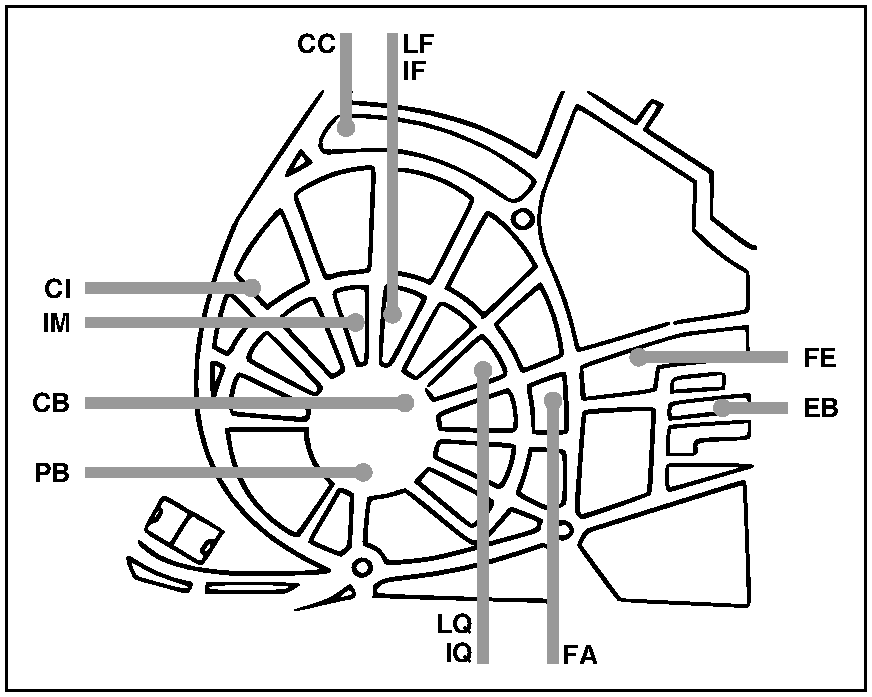
\includegraphics[width=\textwidth]{img/unicamp/mapa_siglas.pdf}
  \caption{Mapa com as siglas da sala de aula}
  \label{fig:mapa_siglas}
\end{figure*}

\subsubsection{SAE (Serviço de Apoio ao Estudante):} É encarregado da execução
de programas de assistência desenvolvidas pela Universidade, por iniciativa
própria ou mediante convênios firmados com entidades especializadas.

\subsubsection{Crédito:} Unidade elementar de horas-aula de qualquer curso da
Unicamp. Um crédito equivale a uma hora-aula semanal, ou a 15 horas-aula
semestrais.

\subsubsection{Período letivo:} É um nome complicado para se referir ao
semestre.

\subsubsection{Currículo pleno:} É o conjunto de disciplinas do curso que o
aluno tem que cursar.

\subsubsection{CR (Coeficiente de Rendimento):} Valor entre 0 e 1 que é a média
das notas obtidas em todas as disciplinas até o momento ponderada pelos
créditos, então ir mal numa matéria de 6 créditos pode prejudicar muito seu CR.

\subsubsection{CP (Coeficiente de Progressão):} É a porcentagem do curso que
você já cumpriu. Por exemplo, se você tem CP = 0,6123 significa que você
cumpriu 61,23\% do curso. Você se forma quando o seu CP for 1 (100\% do curso
completo). É importante saber o CP quando for fazer algum estágio, ou um TCC
(Trabalho de Conclusão de Curso), ou quando for cursar disciplinas que tenham
como pré-requisito AA4xy.

\subsubsection{CPF (Coeficiente de Progressão Futuro):} Além do CP, também tem
o CPF, que além do nome de um documento é o CP que você terá no fim do semestre
caso passe em todas as disciplinas.

\subsubsection{CPE (Coeficiente de Progressão Exigido):} Além do CP e do CPF há
o CPE. O CPE foi instituído a partir de 2005 e é usado para fins de
cancelamento, ou não, de matrícula. Para que o aluno possa continuar a fazer o
curso, ele precisa ter um CP maior ou igual ao CPE daquele semestre. Tanto o
CP, como o CPE e o CPF existem somente nos cursos de graduação.

\subsubsection{Pré-requisito:} Matéria(s) que precisa(m) ter sido cursada(s)
para que se possa fazer outra(s) matéria(s). Existem dois tipos de
pré-requisitos: Os pré-requsitos totais, mais comuns, do qual é exigido tanto a
aprovação por nota como por frequência e os pré-requisitos parciais, mais
raros, do qual o aluno não precisa ter sido aprovado por nota, mas tem que ter
tido aprovação por frequência e nota final maior ou igual a 3,0. Os
pré-requisitos parciais são identificados com um asterisco na frente do código
da disciplina (não confundir com um apontador, uma ferramenta com a qual você
logo irá entrar em contato).

\subsubsection{AA4xy:} Um tipo de pré-requisito. Não se trata de nenhuma
disciplina. Para fazer disciplinas com esse pré-requisito, o aluno tem que tem
um CP maior ou igual a 0,xy.

\subsubsection{AA200:} Outro tipo de pré-requisito existente, mais presente em
disciplinas eletivas. Também não se trata de nenhuma disciplina. É apenas uma
autorização da coordenadoria do curso. Se sobrar vagas para a disciplina e a
coordenadoria do curso for com a sua cara você faz a disciplina.

\subsubsection{PB (Prédio Básico)} Também conhecido como Ciclo Básico II, é um
prédio com várias salas de aula, que fica em frente ao Bandejão, e serve várias
unidades que não possuem espaço físico suficiente para comportar seus alunos.
No segundo andar ficam as salas de aula (PB01 a PB12) e no terceiro andar ficam
os auditórios (PB13 a PB18).

\subsubsection{CB (Ciclo Básico I):} Tem finalidade idêntica ao PB, só que é
muito melhor equipado, tem uma acústica muito melhor e tem um ar condicionado
capaz de matar esquimó de frio. Fica na mesma praça que o PB, só que no outro
extremo. À esquerda da entrada pela rua ficam as salas ímpares e à direita
ficam as salas pares. No primeiro andar ficam os auditórios (CB01 a CB06) que
possuem 140 e 160 lugares e no segundo andar ficam as salas de aula (CB07 a
CB18) que possuem 60 e 80 lugares.  O CB e o PB são os lugares onde você vai
ter a maioria das suas aulas (especialmente nos dois primeiros anos de curso,
então não tem porque procurar morar perto do IC ou da FEEC, cuidado!).

\subsection{Siglas de salas de aula}

A Tabela~\ref{tab:institutos} contém algumas siglas de salas de aula que
aparecem nos cadernos de horários, disponibilizados pelas coordenadorias dos
cursos e pela DAC. E a Figura~\ref{fig:mapa_siglas} aponta a localização das
salas de aula pelas siglas.

\begin{table*}[ht!]
\centering
\begin{tabular}{|c|p{.4\textwidth}|p{.45\textwidth}|}\hline
    \multicolumn{3}{|c|}{ \textbf{Siglas e locais das Salas de Aula no
    horário}}\\ \hline

    \textbf{Sigla}  &  \textbf{Local}  &  \textbf{Referência}\\ \hline

    CB  &  Ciclo Básico I  &  Praça Central, atrás do Santander, em frente à
    Cantina da Física.\\ \hline

    CC  &  Instituto de Computação (IC)  &  Ao lado do Departamento de Artes
    Cênicas (IC-1); ao lado do IE (IC-2) e atrás do IE (IC-3).\\ \hline

    CI  &  Centro de Estudo de Línguas (CEL)  &  Atrás do IFCH.\\ \hline

    CL  &  Instituto de Estudos da Linguagem (IEL)  &  Em frente a praça
    central e ao lado do IFCH.\\ \hline

    EB  &  Engenharia Básica  &  Atrás da Praça da Paz e próximo à FEEC.\\
    \hline

    EM  &  Faculdade de Engenharia Mecânica (FEM)  &  Atrás do IQ.\\ \hline

    FA  &  Faculdade de Engenharia de Alimentos (FEA)  &  Em frente ao IQ e à
    Praça da Paz.\\ \hline

    FE  &  Faculdade de Engenharia Elétrica e de Computação (FEEC)  &  Em
    frente à Praça da Paz.\\ \hline

    IB  &  Instituto de Biologia (IB)  &  Entre o IQ e o Serviço Social do
    SAE.\\ \hline

    IE  &  Instituto de Economia (IE)  &  Atrás do IMECC.\\ \hline

    IF  &  Instituto de Física (IFGW)  &  Em frente ao Ciclo Básico, e a
    Química.\\ \hline

    IH  &  Instituto de Filosofia e Ciências Humanas (IFCH)  &  Entre o IMECC e
    o IEL.\\ \hline

    IM  &  Instituto de Matemática, Estatística e Computação Científica (IMECC)
    &  Em frente a Praça Central.\\ \hline

    IQ  &  Instituto de Química (IQ)  &  Entre o IB e o IFGW.\\ \hline

    LE  &  Laboratórios de informática da FEEC  &  Em frente a Praça da Paz e
    ao lado das salas de aula da FEEC.\\ \hline

    LF  &  Laboratório de Física  &  Em frente à cantina do IMECC.\\ \hline

    LQ  &  Laboratório de Química  &  Em frente à biblioteca do IQ.\\ \hline

    PB  &  Ciclo Básico II, Prédio Básico  &  Praça Central, em frente ao
    Bandejão.\\ \hline
\end{tabular}
\caption{Siglas das salas de aula}
\label{tab:institutos}
\end{table*}

\newpage
%%%%% Lugares para estudar
% Este arquivo .tex será incluído no arquivo .tex principal. Não é preciso
% declarar nenhum cabeçalho

\section{Lugares para estudar}

Há vários lugares para estudar na Unicamp. Vo\-cê pode escolher o que você
achar melhor:


\subsubsection{Biblioteca Central (BC):} A BC tem três andares. O primeiro é
onde tem os livros gerais e onde a galera estuda. Geralmente é barulhento em
épocas de provas, mas é bom porque sempre tem lugar para estudar e fecha às
22h. Se você não se importa com barulho, ou até acha que você faz bastante,
esse é o lugar da BC para você estudar. O segundo andar é onde está a BAE, a
Biblioteca da Área de Engenharia. Um pouco mais silenciosa que a BC nas mesas
externas, esse andar tem salas para estudo em grupo, bastante silenciosas, mas
que sempre estão ocupadas em época de provas, e mesas individuais escondidas
entre os periódicos. O terceiro andar é para silence freaks. Morbidamente
silencioso, desértico (muita gente desconhece a existência desse andar), esse é
o lugar mais silencioso da BC para estudar. Tem umas salinhas de estudo
individual e duas mesas para estudo em grupo. O problema é que fecha às 17h e o
ar-condicionado não é tão bom, mas o pôr-do-sol de lá de cima também é
ma-ra-vi-lho-so.

\begin{figure}[h!]  \centering
  \includegraphics[width=.45\textwidth]{img/unicamp/mesinhas.jpg}
\end{figure}

\subsubsection{Arcádia (ou mesinhas do IEL):} A Arcádia é algumas mesas ao ar
livre no IEL (Instituto de Estudos da Linguagem). Em horários de aula é
silencioso, é um ambiente muito agradável e por ser ao ar livre, não fecha. Tem
dois problemas: O grande fluxo de pessoas no local pode facilmente distraí-lo,
principalmente se você as conhecer, e à noite enche de insetos (além da
iluminação não ser das melhores). Às vezes, venta bastante e é ruim para
estudar com folhas avulsas. Mas ainda assim é um ótimo local para estudar.

\subsubsection{Biblioteca do IFGW:} A biblioteca do IFGW (Instituto de Física
Gleb Wataghin) é ótima para dias de calor, por ser super gelada (
ar-condicionado mega-super-power!). Tem vantagem sobre as outras bibliotecas
pelo fato das salas de estudo serem fora da biblioteca e por isso você não
precisa deixar o seu material para entrar na sala de estudos. Recentemente
reformada, agora conta com 6 salas para estudo em grupo e quantidade razoável
de baias individuais, algumas com tomadas onde você pode plugar seu notebook.
As salas em grupo passaram a ficar trancadas, é preciso deixar o RA pra pegar a
chave, e algumas são reservadas para alunas e alunos da Física.

\subsubsection{BIMECC:} A biblioteca do IMECC tem poucos lugares, poucas mesas
para estudo individual, os locais de estudo ficam dentro da biblioteca (você
precisa guardar sua bolsa para entrar), não é muito gelada, as tomadas são
concorridas e o ambiente não é agradável, mas nela e na BAE é que você
encontrará a maioria dos livros relacionados a computação.

\subsubsection{Outras bibliotecas:} Aventure-se por outras bibliotecas, como a
da Economia, a da Pedago, a da Química -- que é muito boa, sobretudo o segundo
andar, é possível conversar baixinho sem atrapalhar -- e a da Biologia e as
conheça. Para aqueles que gostam (ou são obrigados) a estudar aos fins de
semana a BC e as bibliotecas da Educação, da Economia, da Química, da Medicina,
do IEL e da Geociências abrem aos sábados. Para saber os horários de
funcionamento das bibliotecas, entre no site do SBU
(\url{bit.ly/2A9ZBC3}).

\subsubsection{Bitolódromos:} Existem um bitolódromo na Unicamp: o da\\FEEC
(coincidência interessante, né?), fica no fundo do prédio principal (qualquer
veterana ou veterano sabe onde é o bitolódromo, não tenha vergonha de
perguntar). Embora pica-fios sejam bastante barulhentos, você sempre encontra
gente que possa te ajudar e o vai-e-vem das pessoas não incomoda tanto, pois
grande parte são desconhecidas. Recentemente abriram um novo bitolódromo na
FEEC, no fim do corredor que leva ao SIFEEC, mas tudo indica que esse espaço é
temporário, talvez ele não exista mais no momento em que você está lendo isso.

% \subsubsection{Sala 316:} Outro alento para as madrugadas de estudo é a sala
% 316 do IC-3, que fica aberta sempre, ou então, aberta facilmente com a chave
%que fica com a/o guardinha. É uma sala com carteiras legais, lousa e ar
%condicionado, aliás, é muito boa para estudo em grupo (NABVS IMINENTVS) por
%causa da lousa.

\begin{figure}[h!]  \centering
  \includegraphics[width=.45\textwidth]{img/unicamp/lua.jpg}
\end{figure}

\subsubsection{Sua casa:} Se você mora em uma república com pessoas da sua
turma, vá fundo e estude em casa. Se você mora sozinha ou com pessoas de
outros cursos/anos, mas se concentra bem em casa, também o faça. Caso
contrário, estude na Unicamp. É muito fácil se distrair em casa. Você vai à
geladeira, mexe no computador, lê outra coisa, deita na cama e dorme, entre
outras coisas. Prefira estudar na Unicamp. Outra coisa, não seja egoísta,
quando tiver oportunidade de estudar em grupo, prefira essa alternativa.
Lembre-se que você não está mais no ``cursinho'', tente sempre pegar as dicas
que a galera te dá, principalmente das suas veteranas e veteranos.

\newpage
%%%%% Cuidado com CR e Reprovação
% Este arquivo .tex será incluído no arquivo .tex principal. Não é preciso
% declarar nenhum cabeçalho

\section{Cuidado com CR e Reprovação}

Durante o curso você vai ouvir que se preocupar com seu CR é bobagem, que
estudar para tirar nota não leva a lugar nenhum, que depois de formada não é
seu CR que te colocará no mercado de trabalho etc. Cuidado, trabalhar numa
empresa não é a sua única opção de vida após formada, e preste atenção, pois
``após formada'' não significa durante o curso.

Durante o curso você vai ter a possibilidade de participar de várias atividades
acadêmicas e algumas delas vão exigir bom aproveitamento acadêmico da aluna ou
aluno. Por exemplo, para se candidatar a monitor de uma disciplina você precisa
ter CR acima do da média da turma. Para pleitear uma bolsa de iniciação
científica, onde há concorrência entre alunas e alunos do país todo, também
será exigido bom aproveitamento, assim como para uma bolsa de mestrado. Caso
você não saiba, mestrado faz parte da pós-graduação, ou seja, o seu CR vai te
influenciar até após formada.

Cuidado também com a reprovação. Há instituições, como a FAPESP (Fundação de
Amparo à Pesquisa do Estado de São Paulo), que é a maior fomentadora de
pesquisas do estado de São Paulo e que paga os maiores valores de bolsas do
país, que te excluem de qualquer disputa só por ter uma reprovação no seu
histórico escolar da graduação. Não te exclui oficialmente, mas como é muito
concorrido por ser a melhor pagadora, seu nome vai para o final da lista.

Parece óbvio que quem estuda tira boas notas, mas até você aprender a estudar
como a universidade exige, pode demorar um pouco, e há pessoas que nunca
aprendem. Ah, e cuidado com o estudo exagerado, é um curso de 4 a 8 anos, não
dá para manter o rítmo de estudo para vestibular -- caso você estudou
fortemente no cursinho ou ensino médio -- por todo esse tempo.

Há certos períodos (semestres), quando você já estiver mais avançado no curso,
em que poderá sentir-se à vontade para desistir de uma disciplina em que esteja
matriculado, deixando para completá-la posteriormente. Quando você fizer isso
há a possibilidade de desistir da disciplina, desmatriculando-se oficialmente.
Mas há pessoas que simplesmente deixam de cursar a disciplina, reprovando por
nota e falta e ficando com uma nota baixa em seu histórico. Cuidado com isso,
pode ser frustrante para você no futuro. Por isso, se for desistir de cursar
uma disciplina após matriculado, sempre peça a desistência e tente não
reprovar.

Lembre-se de que o período de graduação é muito grande, você pode mudar de
ideia a qualquer momento sobre o que pretende fazer no futuro.

\newpage
%%%%% Pra que que eu estou estudando isso??
% Este arquivo .tex será incluído no arquivo .tex principal. Não é preciso
% declarar nenhum cabeçalho

\section{Para que eu estou estudando isso?}

O ensino médio acabou, você finalmente está livre de todas as ``inutilidades'',
como química orgânica e separação silábica de verbos parnasianos, só vai ver
coisas relevantes para a profissão, e{\dots}

Pimba! HZ291. Pode, Arnaldo?

Primeiro, você precisa saber que a Universidade não é um curso técnico. A ideia
não é só te dar capacitação profissional, mas sim formar pessoas melhores. Para
que uma computeira ou um computeiro precisa de contabilidade? Para nada, mas
uma pessoa precisa ter uma noção disso, sobretudo de exatas.

Outro problema: o que exatamente é ``relevante para a sua profissão''?  A
computação é uma área muito vasta, e a graduação é muito generalista, para te
dar base para escolher. Por exemplo, vai ter gente que nunca mais vai usar
GA/Algelin -- geometria analítica e álgebra linear --, mas quem for para a área
de computação gráfica vai comer matriz no café da manhã. Quem garante que, no
meio do curso, você não decida ir para essa área? Ou ainda, que no seu emprego
não te joguem um problema desse tipo?

Se você continuar na universidade, na pós-graduação, você só terá matérias da
sua área, já que você já sabe o suficiente pra dizer que área é essa. Mas ainda
falta muito chão até lá{\dots}

Para quem é da engenharia, para conseguir o CREA, existem algumas matérias
obrigatórias, como resistência dos materiais. A Unicamp pode até contrariar
essas orientações, até certo ponto -- e ela o faz: as coordenadoras e
coordenadores da engenharia tem lutado para diminuir créditos obrigatórios e
aumentando eletivos --, mas há matérias em que as professoras e professores
dificilmente concordariam em alterar. (Por outro lado, você poderá construir
prédios de até 2 andares. Recomendamos fortemente que você não faça isso.)

Tanto para a ciência quanto para a engenharia, o curso não é para formar
simples programadores. Vocês serão mais que isso, serão cientistas, engenheiras
e engenheiros, e isso envolve ver coisas além de computação.

\newpage
%%%%% Bem-vindo à academia
% Este arquivo .tex será incluído no arquivo .tex principal. Não é preciso
% declarar nenhum cabeçalho

\section{Bem-vindo à academia}

Academia é o nome que se dá à comunidade internacional de pesquisadores e
estudantes de ensino superior, atuando em todas as áreas do conhecimento.
Geralmente centrada ao redor de universidades, porém organizações públicas e
privadas e também empresas fazem parte. A Academia é dividida principalmente
entre os pilares de Pesquisa, Ensino e Extensão, sendo os dois primeiros mais
acessíveis para nós da graduação.

A Unicamp está muito bem situada no cenário acadêmico, sendo a responsável por
15\% da produção científica brasileira, e tendo inúmeros pesquisadores de
renome internacional, então não vão faltar oportunidades para você entrar nesse
mundo.

\subsection{Iniciação Científica}

A iniciação científica é um tempo para alunas e alunos de graduação (você, no
caso) ter uma experiência acadêmica mais séria, sentir um pouco como é o clima
de pesquisa. Interessou? O que fazer? Calma, você mal entrou na Universidade.
Geralmente, o que se faz é conversar com professoras e professores da área com
a qual você se identifica mais (criptografia, teoria da computação,
processamento de imagens, inteligência artificial, física, química etc.) e ver
se está desenvolvendo algum projeto interessante naquela área, ou propor alguma
ideia sua mesmo. Depois você começa a estudar para redigir um projeto e
encaminhá-lo para alguma instituição de fomento à pesquisa (CNPq ou FAPESP),
pedindo uma bolsa de iniciação científica. A FAPESP paga em torno de R\$ 640,00
e aceita pedidos de bolsa em qualquer período do ano. O CNPq paga
aproximadamente R\$ 400,00, e o período para inscrição de projetos é geralmente
em junho e novembro. No primeiro semestre geralmente é bem mais difícil achar
alguma professora ou professor da área que você se interessa, aliás, é bem
difícil saber a área com a qual você se identifica, pois você mal começou o
curso e não conhece muito do que se estuda em computação, muito menos os
professores. Mas tenha paciência, agora parece tudo muito complicado, mas com o
tempo as coisas vão ficando mais simples. Se você realmente tiver uma sede
insaciável de conhecer o meio da pesquisa, procure a professora ou professor
que te deu aula de MC102, ele pode te orientar a respeito.

\begin{figure}[h!]
  \centering
  \includegraphics[width=.45\textwidth]{img/unicamp/congresso.jpg}
  \caption*{Congresso de Iniciação Científica da Unicamp}
\end{figure}

Outra coisa interessante a respeito da iniciação científica é que, se você
conseguir bolsa, pode pegar a disciplina MC040 e posteriormente MC041 (2
semestres), cada uma com 12 créditos. São 24 créditos praticamente ``de
bandeja'' para ajudá-la a recuperar o CR, caso esteja no fundo do poço. Note
bem as aspas. Os trabalhos de iniciação científica geralmente consomem muito
tempo de estudo e dedicação, não vá pensando que é moleza, não.

Na FEEC, você pode conseguir as matérias de iniciação (EA002 até EA005) mesmo
sem bolsa, mas você ainda assim vai precisar de um orientador. Lá a iniciação
científica também substitui o estágio, mas não tem equivalência com a do IC.

Note que sua iniciação científica não precisa estar vinculada a computação.
Como falaremos ainda neste capítulo, a Unicamp permite que você faça
disciplinas de qualquer instituto com créditos eletivos, isso pode te estimular
a fazer matérias de áreas que gosta fora da computação e nada te impede de
fazer alguma iniciação científica nisso, aproveite!

\subsection{Monitoria}

Além da iniciação científica, monitoria é uma forma muito comum de participar
da Academia, mais focado no pilar de ensino. Não vai demorar muito para você
descobrir a importância da monitoria para as matérias. Logo no primeiro
semestre, boa parte das disciplinas possuem monitoras ou monitores, que são
dividos em dois tipos: PED (Programa de Estágio Docente) e PAD (Programa de
Apoio Didático).

\textbf{PED} é alguém da pós-graduação que é responsável por ajudar a
professora ou professor na disciplina, normalmente, criando materiais,
exercícios, laboratórios e ajudando na correção dos mesmos. Já \textbf{PAD} é
alguém da graduação e geralmente só é responsável por ajudar nos laboratórios e
tirar dúvidas, não deve incluir correção de trabalhos.

Por enquanto, o mais importante pra quem quer participar é o PAD. Todo mundo
pode se inscrever, a forma e momento das inscrições varia de acordo com o
instituto, mas costuma ser no final do semestre. No IC e FEEC, recebemos um
e-mail da Secretaria de Graduação com um formulário para preencher.

O programa de PAD costuma incluir uma bolsa que fica em torno de R\$ 520,00.
Os pré-requisitos pra conseguir são (1) ter cursado a disciplina ou alguma
equivalente, (2) não ter reprovado na disciplina e (3) ter disponibilidade para
participar das atividades, que para o nosso curso costuma ser estar livre
durante os laboratórios, (4) ter o CR acima da média da sua turma ou ter a
maior nota na matéria dentre os candidatos.

Algumas disciplinas são mais concorridas que outras para monitoria, como é o
caso das primeiras matérias da computação. Algo interessante é que, assim como
iniciação, monitoria também tem duas disciplinas, MC050 e MC051 -- ambas de 8
créditos. Mesmo sem bolsa, é possível exercer monitoria, conseguindo os
créditos.

Mas vá com calma, como é preciso ter cursado a disciplina e ter um CR para se
candidatar pra monitoria, só vai ser possível se candidatar no final do seu
segundo semestre, já que as inscrições acontecem no fim do semestre (geralmente
próximo da matrícula). É bom se atentar que monitoria exige um certo tempo de
dedicação, em especial porque você estará ajudando outras alunas e alunos na
disciplina. É uma grande responsabilidade e uma ótima forma de ter contato com
um dos lados da Academia que muitas vezes é esquecido: justamente o lado que
lhe trouxe para cá!

\subsection{PIF -- Programa Integrado de Formação}

O PIF é uma oportunidade das alunas e dos alunos de graduação de adiantarem
créditos da pós-graduação no IC enquanto estão na graduação. É uma boa ideia
mesmo que sua intenção não seja fazer pós, pois é automático, simples e, além
disso, nunca sabemos quais serão nossas vontades no futuro.

Para participar, a aluna ou o aluno de graduação de computação precisam possuir
CR e CP maiores que 0,6. A inscrição é automática, ou seja, cumprindo esses
pré-requisitos, poderá cursar maté\-rias da pós-graduação como graduanda. Para
apro\-veitar os créditos no futuro, como pós-graduanda, no entanto, é necessário
realizar uma inscrição na DAC para se tornar um aluno ou uma aluna especial de
pós-graduação. E essa inscrição não apresenta o compromisso da aluna ou do
aluno em terminar a pós.

Você pode entender mais sobre esse programa em:

\begin{center}
\url{www.ic.unicamp.br/ensino/pg/info/pif}
\end{center}


\subsection{Intercâmbio}

A Unicamp é uma das universidades brasileiras que têm maior prestígio fora do
país e a VRERI-Unicamp (Vice-Reitoria Executiva de Relações Internacionais,
antigo CORI), IC e FEEC têm vários acordos bilaterais de intercâmbio. Então,
para você que quer dar um salto em algum idioma, conhecer outras culturas e
sentir na pele a aventura de ser estrangeira, comece a se preparar desde já.

Muita gente costumava pegar intercâmbio pelo Ciência Sem Fronteiras, mas ele
foi congelado pelo Governo Federal em 2015, e passou por uma reformulação: não
haverá mais vagas para a graduação, apenas para a pós. Ainda existem boas
opções pra quem gostaria de pegar um intercâmbio, mas ficou muito mais difícil.

A França hoje recebe um número razoável de estudantes de computação, devido a
acordos que a Unicamp tem com os INSA e com as Écoles Centrales e também graças
a bolsas de estudo oferecidas pela Capes e pelo governo francês. Os
intercâmbios para a França são bem mais concorridos que o Ciência sem
Fronteiras, pois são na modalidade de duplo diploma (você se forma pela Unicamp
e pela instituição francesa), há um processo seletivo envolvendo uma
entrevista, e vai durar mais tempo, dois anos ou mais, numa instituição de
prestígio como a École Polytechnique, por exemplo.

No site da VRERI existem oportunidades para ir para Estados Unidos, Japão,
América Latina, Alemanha, Espanha etc., muitos com boas bolsas de estudo ou com
incentivos que valem a pena caso você tenha um pouco de grana para se sustentar
no início. Visite sempre o site da VRERI e participe das reuniões que ela faz,
pois ficar ligada é a chave para conseguir encontrar uma boa oportunidade.
Existem outras opções de intercâmbio, como a AIESEC, que promove um intercâmbio
para estágios no exterior. Se seu interesse é mais profissional, procure se
informar.

\begin{quote}
``Mas vale a pena? Poxa, vou atrasar meu curso, ficarei deslocada de turma, vou
ficar em um país estranho, para quê? Acho que não vale a pena{\dots}''
\end{quote}

Vamos começar pelos motivos profissionais: ter no currículo que você fala uma
língua estrangeira fluentemente devido à sua imersão no país é algo muito
valorizado pelas empresas, além do fato que o pessoal do RH vai ver que você
tem capacidade de se virar sozinha, uma vez que não é tão óbvio sair do país e
recomeçar sua vida fora. Você não atrasará tanto seu curso, pois a Unicamp
conta com um sistema de equivalências de matérias, e se você escolher bem pode
fazer matérias que serão convalidadas na Unicamp. Agora, o que realmente é
importante: você está na faculdade, está na hora de deixar o colo da mamãe e
partir para o mundo! A experiência de conhecer outras culturas, criar laços de
amizade internacionais, viajar por terras desconhecidas não tem preço! Pense
que é no seu tempo de facul que terá oportunidade de fazer uma aventura destas,
não desperdice.

Se você abriu um sorriso e pensa que está preparado para sair do país, comece a
estudar, bixete! Não que ter uma boa nota seja a única forma de conseguir uma
vaga em uma bolsa de estudos, mas com certeza é a mais fácil. Busque atirar em
todas as frentes, mantenha seu CR num bom nível, busque conhecer organismos
como AIESEC e procure grupos de trabalho (no IC existem vários) que podem levar
alunos ao exterior. Boa sorte!

Se você realmente se interessou, aí vão uns links com mais informações:

\begin{itemize}
\item VRERI:
  \begin{small}
  \url{www.internationaloffice.unicamp.br}
  \end{small}
\item AIESEC: \url{aiesec.org.br}
\end{itemize}

Fique atenta aos e-mails que você receberá do IC e da FEEC. Alguns deles são
sobre programas de intercâmbio.

\subsection{Acesso a artigos e revistas científicas}

Os resultados de pesquisas científicas, no Brasil e no mundo, costumam ser
publicados por meio de periódicos e conferências, os quais normalmente são
disponíveis pela internet.

No Brasil, quase todas as instituições públicas de ensino superior, como a
Unicamp, participam de um sistema conhecido como \textbf{Portal de Periódicos
da Capes} (\url{periodicos.capes.gov.br}), que garante acesso a grande parte
das publicações científicas das principais editoras do mundo sem necessidade de
pagar nada a mais por isso.

Nas áreas de engenharia e de computação, quase todas as publicações relevantes
são acessíveis através desse sistema. Mas é importante você saber que esse tipo
de acesso só é possível a partir de endereços IP da Universidade, então se você
quiser acessar algum artigo quando estiver em casa, o ideal é usar o sistema de
acesso VPN (Virtual Private Network) disponibilizado pela Unicamp, como pode
ser visto no site: \url{bit.ly/1xHdH8X}.

Através da \textbf{Comunidade Acadêmica Federada (CAFe)}, foi disponibilizado
recentemente um método de acesso remoto aos periódicos sem necessidade de usar
a VPN, mais informações aqui: \url{bit.ly/1w1twlz}

Na Unicamp, você ainda tem acesso a diversas outras publicações e e-books que
não são cobertos pelo sistema da Capes, além de alguns periódicos impressos,
que podem ser encontrados nas bibliotecas. Caso você queira buscar algo no
material que há disponível física ou virtualmente na Universidade, acesse o
site do \textbf{Sistema de Bibliotecas da Unicamp}: \url{www.sbu.unicamp.br}.

Para uma busca mais abrangente de artigos científicos na internet, você pode
usar o \textbf{Google Acadêmico} (\url{scholar.google.com}). Mas atenção! Você
pode encontrar artigos que não são cobertos pelo Portal da Capes nem pela
Unicamp e exigem pagamento.

Além do Portal de Periódicos, existe também um novo modelo de publicações
científicas de acesso gratuito, chamado \textbf{open access}. Esse modelo tem
origem muito próxima do movimento pelo software livre. Publicações feitas nesse
sistema são acessíveis a qualquer momento, de qualquer IP e sem qualquer custo.
Alguns exemplos de grandes repositórios e editoras open access são:

\begin{itemize}
\item \textbf{SciELO:} \url{www.scielo.org}
\item \textbf{PLOS:} \url{plos.org}
\item \textbf{arXiv:} \url{arxiv.org}
\item \textbf{PMC:} \url{ncbi.nlm.nih.gov/pmc}
\end{itemize}

A rede \textbf{SciELO} é onde a maior parte dos artigos em português é
publicada. O acervo \textbf{PMC} é de publicações da área biomédica.

Bixete, guarde bem esta seção do manual! Pode ser que você não vá usá-la logo
de cara, mas quando você fizer iniciação científica ou um trabalho de
disciplinas mais avançadas, você aproveitará bastante essas informações.

\newpage
%%%%% Modalidades da engenharia de computação
% Este arquivo .tex será incluído no arquivo .tex principal. Não é preciso
% declarar nenhum cabeçalho

\section{Modalidades de engenharia da computação}

Às engenheiras e aos engenheiros, esta seção serve para dar uma breve
explicação sobre as duas modalidades de graduação em engenharia de computação.
Mas, primeiro, {\emph{``o que é uma modalidade?''}} Uma modalidade é uma
subdivisão do curso de engenharia, um enfoque específico da sua formação. São
catálogos alternativos que visam distribuir diferentes disciplinas para a mesma
formação, ou seja, possui ênfases em áreas diferentes para se formar em
engenharia de computação. Há duas modalidades: AA, Sistemas de Computação, e
AB, Sistemas e Processos Industriais.

Uma das características da Unicamp é dar ao aluno uma formação \textbf{MUITO}
generalista, então todas as alunas e alunos, independente da modalidade -- ou
sendo até da ciência --, estarão capacitados a atuar em qualquer área da
computação. Assim, a escolha da modalidade é apenas um modo de dar à aluna e ao
aluno a oportunidade de se aprofundar em assuntos que lhe interessem. É
importante ressaltar que ambas as modalidades têm uma grande parte de
disciplinas em comum, então a formação básica é essencialmente a mesma. Perto
do período de escolha, o CACo lhe dará mais detalhes no conjunto de palestras
sobre as modalidades AA e AB que são realizadas no segundo semestre para sanar
todas as suas dúvidas e auxiliá-la.

Observação: não escolha sua modalidade por conta do IC ou da FEEC ficarem mais
próximas da sua casa, por favor{\dots}

\subsection{Modalidade AA: Sistemas de Computação}

Também conhecida como Azóide, é a que mais se assemelha à ciência da computação
por focar mais nas áreas de análise e projeto de algorítmos, matemática
discreta e arquitetura de computadores. As aulas serão ministradas
majoritariamente pelo IC.

\subsection{Modalidade AB: Sistemas e Processos Industriais}

Também conhecida como Bzóide, um pouco mais próxima da engenharia elétrica por
conta da conexão com análise de sinais, sistemas autônomos, embarcados. As
aulas serão oferecidas majoritariamente na FEEC.\\ % pulamos mais uma linha ;)

{\emph{``E como mudo de modalidade?''}} A não ser que você tenha concluído 110
créditos dentre as matérias da modalidade desejada, só mudará de modalidade no
quarto semestre, com um pedido na DAC durante o período de matrícula ou
alteração de matrícula.

Ah, como a Unicamp te dá a oportunidade de escolher livremente suas matérias,
você pode mesclar matérias tanto oferecidas para Azóides quanto para Bzóides
verificando com veteranas e veteranos como foram os oferecimentos de cada lado
e escolhendo o que mais lhe agrada, mas tome cuidado com a questão da
equivalência de disciplinas: ás vezes alguma matéria Azóide não completa a
matéria Bzóide e vice-versa!

\newpage
%%%%% Emails acadêmicos
% Este arquivo .tex será incluído no arquivo .tex principal. Não é preciso
% declarar nenhum cabeçalho

\section{Agora eu tenho um e-mail da Unicamp}

Ao ingressar num curso de computação, você recebe pelo menos três contas de
e-mail: do IC, da DAC e do Google Apps for Education. Os dois primeiros são os
principais meios de comunicação da universidade com você, portanto fique
esperta e não deixe de ler esses e-mails regularmente!

Para acessar o webmail do IC, o endereço é
\\\urls{https://webmail2.students.ic.unicamp.br}. O login e a senha são os
mesmos do sistema Linux do IC, que você receberá nas primeiras semanas de
aula de laboratório. Caso tenha dúvidas, dê uma passada na Secretaria de
Graduação, que fica no IC-2 (prédio ao lado das Artes Cênicas e para cima da
Economia) e pergunte!

Uma dica interessante, que muitas vezes passa despercebida, é que no mesmo
documento em que você recebe sua senha, vem indicado um \textit{alias} para o
seu e-mail. Assim, você poderá utlizá-lo de uma forma mais amigável, ao invés
de ser somente o seu próprio RA, por exemplo:

\begin{center}
\texttt{francisco.silva@students.ic.unicamp.br}\\
ao invés de\\
\texttt{ra129873@students.ic.unicamp.br}
\end{center}

O webmail da DAC é a primeira letra do seu nome, seguido dos dígitos do RA e do
sufixo:
\begin{center}
\texttt{dac.unicamp.br}
\end{center}
O e-mail da DAC também é útil. É nele que você será avisada sobre o período
de matrícula, pedidos de matrículas provisórias, avisos de desistências e
trancamentos, além de te informar a respeito de eventos que acontecem na
Unicamp, como feiras, palestras, festivais, eleições. O endereço do webmail da
DAC é \url{webmail.dac.unicamp.br}.

Outro e-mail que também está disponível para as alunas e alunos é uma conta no
Gmail, devido a uma parceria entre a Unicamp e a Google! Mais informações sobre
como acessar e o que ganhamos com isso na seção de servicos da Unicamp, no
final do manual.

Para a galera da engenharia, ainda há o da FEEC, que muitos sequer ficam
sabendo que existe! Só após um semestre ou até um ano depois vão até o SIFEEC
retirar seu login e senha. Ou então ficam sabendo só no segundo ou terceiro ano
de curso e aí há mais de 700 e-mails não lidos. Assim como o do IC, é muito
utilizado para divulgação de eventos, oportunidades de estágios e de iniciação
científica. Para utilizá-lo, você deve ir até a FEEC e procurar o SIFEEC, que é
o local responsável por isso. Fica no segundo andar do prédio de laboratórios
da FEEC (um com escadas amarelas). O endereço do webmail da FEEC é
\url{webmail.fee.unicamp.br} e a senha é a mesma do Linux da FEEC.

\begin{figure}[b!]
  \centering
  \includegraphics[width=.3\textwidth]{img/alem_da_graduacao/email.jpg}
\end{figure}

Você também pode redirecionar os e-mails que receber nas contas do IC, FEEC e
DAC para qualquer outra conta (no Gmail, por exemplo).

\subsection{Redirecionamento de e-mails}
Para efetuar o redirecionamento do e-mail institucional para outro e-mail, siga
os passos abaixo para cada e-mail institucional que você tiver.

\subsubsection{E-mail da DAC}

\begin{compactenumerate}
\item Acesse \url{www.dac.unicamp.br}
\item Acesse Estudantes
\item Acesse E-mail e ferramentas Google
\item Faça login
\item Clique no ícone de engrenagem na parte superior direita
\item Clique em Configurações
\item Clique em Encaminhamento e POP/IMAP
\item Clique em Adicionar um endereço de encaminhamento
\end{compactenumerate}

\subsubsection{E-mail da FEEC}

\begin{compactenumerate}
\item Acesse \url{webmail.fee.unicamp.br}
\item Faça login
\item Acesse Options
\item Acesse Mail Forwarding
\end{compactenumerate}

\subsubsection{E-mail do IC}

O IC disponibiliza 2 sistemas de e-mail, disponibilizados em 2 endereços. Para
facilitar sua vida, utilize este primeiro, que é o mais atualizado:

\begin{compactenumerate}
\item \urls{https://webmail2.students.ic.unicamp.br}
\item Faça login
\item Na seção Filtros, clique em Encaminhar
\item Coloque seu endereço de email no campo e grave as mudanças.
\end{compactenumerate}

\begin{compactenumerate}
\item \urls{https://webmail.students.ic.unicamp.br}
\item Faça login
\item Na seção Filtros, adicionar nova regra
\item Mude a condição para ``All''
\item Mude ação para redirecionar
\item Coloque seu endereço de email no campo e aplique as mudanças.
\end{compactenumerate}

\subsection{Suporte técnico}

Além dos serviços de e-mails, ao entrar na Unicamp, você também ganha acesso a
diversos outros serviços, como a VPN da Unicamp, acesso remoto ao IC etc.

Obviamente configurar essas coisas não é trivial, o IC mantem uma página com
instruções de como usar os seus serviços comuns, como configurar seu cliente de
email para acessar o servidor do IC e acessar o IC remotamente.

Sempre que precisar de ajuda no IC, confira se não há uma resposta para seu
problema nesta página:\\
\url{suporte.ic.unicamp.br/index.php/Alunos}

% TODO: Encontrar informações sobre o suporte da FEEC e da DAC.

\subsection{Tenha uma conta no Gmail!}

Nós sabemos que é difícil. Muitas vezes você vem usando um serviço de e-mail
durante anos, seja ele Hotmail, Yahoo, Uol, Terra, Zipmail, e mudar é
trabalhoso. Mas confie na gente: agora vai ser mais fácil. Você está começando
uma vida nova na universidade, quando já tiver cadastrado seu endereço antigo
em vários serviços acadêmicos e divulgado entre os novos contatos que vai
fazer, será bem mais complicado.

Entre as vantagens do Gmail, podemos destacar:

\begin{compactitemize}
\item Muito espaço, nunca mais apague nada;
\item visualização em threads, útil para acompanhar discussões;
\item bom aplicativo para smartphones;
\item filtros e marcadores infinitos para te ajudar;
\item uma pesquisa que funciona;
\item interface mais polida que as da concorrência.
\end{compactitemize}

\emph{Até a Unicamp} está tentando te obrigar a usar Gmail, como dissemos!
\shrug

Qualquer dúvida, novamente, procure uma veterana ou veterano!

Finalizando, não deixe de estar sempre informado sobre os acontecimentos ou
divulgações da Unicamp, do CACo, da AAACEC e da Conpec, essas três entidades
compostas por alunas e alunos de computação.

O CACo mantém uma lista de email para discussão geral de coisas relacionadas à
computação e à Unicamp em \url{bit.ly/cacounicamp}.

\newpage
%%%%% Melhores banheiros
% Este arquivo .tex será incluído no arquivo .tex principal. Não é preciso
% declarar nenhum cabeçalho

\section{Melhores banheiros}

Uma das maiores necessidades do ser humano pode ser potencializada se for
realizada num banheiro decente. Portanto, é muito importante que você saiba
onde ir. Alguns dos melhores banheiros da Unicamp são:

\subsubsection{IC-3:} Geralmente estão limpos e utilizáveis, mas fedem. E em
dia de chuva ficam imundos. Exceto nos finais de semana, sempre possui papel
higiênico: é uma boa pedida na hora do apuro.

\subsubsection{IC-3,5:} Os banheiros do térreo não são flor que se cheire, porém
devido à localização um pouco mais distante, pode ser suficiente se você prefere
um pouco mais de privacidade. O grande segredo são os banheiros da
pós-graduação, localizados no primeiro andar. Estes são ainda menos
frequentados e a qualidade é extremamente superior aos do andar inferior. Além
disso, a torneira é excelente à quem gosta de escovar os dentes depois do
almoço. Nesses casos, subir algumas escadas compensa bastante.

Observação: quando o bebedouro perto dos laboratórios possui um gosto na água, o
bebedouro do primeiro andar do IC-3,5 tem uma vazão excelente e é um ótimo
substituto.

\subsubsection{IC-2:} Quase sempre estão limpos e utilizáveis e tem um odor
melhor que os do IC-3. Só precisa tomar cuidado pois às vezes falta papel
higiênico.

\subsubsection{FEEC:} Possui excelentes banheiros escondidos por lá,
principalmente após as reformas de 2013. Procure bem!

\subsubsection{PB:} Os banheiros do segundo e do terceiro andar do Pavilhão
Básico são muito melhores que os do térreo (especialmente os do terceiro andar,
por quase não serem usados). Só tome cuidado, porque às vezes não tem papel
higiênico.

\subsubsection{FE:} A Faculdade de Educação tem poucos banheiros masculinos.
Estão entre os melhores da Unicamp pelo pouco uso.

\subsubsection{CB:} Estes banheiros ficam escondidos próximo às escadas do CB
(no térreo). Se você tiver sorte de chegar bem após a limpeza, o banheiro
estará em excelentes condições. Porém, na maior parte do tempo, ele fica bem
sujinho.

\subsubsection{DEQ:} Departamento de Eletrônica Quântica, no IFGW. Dizem que
ninguém os usa.

\subsubsection{DRCC:} Departamento de Raios Cósmicos e Cronologia, no IFGW. Um
dos melhores banheiros existentes na Unicamp (senão o melhor). Assim como os
banheiros do DEQ, dizem que ninguém os usa.

\subsubsection{DFA:} Departamento de Física Aplicada, no IFGW. Os dois andares
do departamento tem banheiros bons e utilizáveis, mas algumas vezes falta
papel higiênico.

\subsubsection{IMECC:} Todos os três departamentos (andares) do\\IMECC tem
banheiros bons e utilizáveis. Mas vez ou outra falta papel higiênico.


\chapter{Além da graduação}
%%%%% Centro Acadêmico da Computação
% Este arquivo .tex será incluído no arquivo .tex principal. Não é preciso
% declarar nenhum cabeçalho

\section{CACo -- Centro Acadêmico da Computação}

\begin{figure}[H]
  \centering
  \includegraphics[width=.35\textwidth]{img/caco_logo.pdf}
\end{figure}

\subsection{O que é um centro acadêmico?}

Bixete, o CACo é o seu centro acadêmico. Um CA é uma entidade estudantil que,
em linhas gerais, deve trabalhar para garantir os interesses de todas e todos
estudantes, melhorando o curso e a faculdade a que pertence. Qualquer pessoa
que se encaixa na descrição anterior é um membro do CACo e isso inclui você.
O CACo é formado pelas alunas e alunos de graduação tanto em engenharia quanto
em ciência da computação da Unicamp, além de pessoas da pós-graduação do IC.

Um centro acadêmico é parte do famoso ``movimento estudantil'' de que você
provavelmente já ouviu falar. Mas não se engane! Pergunte para o seu pai o que
ele pensa quando lê ``movimento estudantil'' e ele vai dizer que vê um bando de
estudantes desocupadas e desocupados associadas a um partido político de
esquerda que saem por aí protestando contra o sistema e queimando ônibus pelas
ruas. Se você pensa assim, mude sua ideia: o CACo não é nada disso.

\begin{figure}[H]
  \centering
  \includegraphics[width=.45\textwidth]{img/alem_da_graduacao/caco_karaoke.jpg}
\end{figure}

O CACo tem como função representar estudantes no âmbito acadêmico, ou seja,
perante o IC, a FEEC e a Unicamp. Mas o que o CACo faz? De forma simplificada,
procuramos ser porta-voz de alunas e alunos. Reivindicamos espaço físico
decente, alteração nas matérias e seus oferecimentos, promovemos discussões
sobre temas polêmicos e delicados, mas também integração e muitas outras
atividades.

Quer um exemplo? Esse estupendo manual que você está lendo neste exato momento
foi confeccionado pelo seu centro acadêmico para lhe ajudar no início da sua
vida universitária e, na verdade, você ainda vai se pegar recorrendo ao seu
manual várias vezes durante seus quatro, cinco, doze anos na Unicamp.

Uma grande função do CACo é prezar pela qualidade dos cursos e fazemos isso,
por exemplo, através de discussões com o próprio Instituto, onde levamos
reclamações e reivindicações para as coordenadoras, professoras, os
coordenadores e professores.

\begin{figure}[H]
  \centering
  \includegraphics[width=.45\textwidth]{img/alem_da_graduacao/caco_reuniao.jpg}
\end{figure}

Uma outra função do CACo é integrar estudantes de computação da Unicamp. Para
isso, realizamos diversos eventos como o CineCACo, o PipoCACo, o CACo Games, o
CACo Series of Poker, o MagiCACo e a grande comemoração do Aniversário do CACo,
que já contou com pizza de graça para mais de duzentas pessoas! Tentamos também
facilitar a vida da galera através dos armários que alugamos, o banco de livros
e o maravilhoso banco de provas, provavelmente o maior da Unicamp, disponível
online.

Repetindo o que foi dito antes: bixete, o CACo é o \textbf{SEU} centro
acadêmico. Tudo que dissemos que fazemos pelas alunas e alunos, queremos fazer
por você também. Por isso, quando houver algum problema envolvendo a FEEC, o
IC, as professoras, os professores ou qualquer coisa do tipo, não hesite em nos
procurar. O CACo sempre lhe dará todo o suporte necessário. Se tiver reclamação
ou sugestão relacionada ao próprio CACo, também estaremos aqui para ouvir. Mais
do que isso, venha participar de uma de nossas reuniões, que são abertas a você
e todas as alunas e alunos de computação da Unicamp.

\begin{figure}[H]
  \centering
  \includegraphics[width=.45\textwidth]{img/alem_da_graduacao/caco_fisl2.jpg}
\end{figure}

\subsection{Como posso participar do centro acadêmico?}

Participar do CACo é uma experiência diferente de tudo aquilo que você terá na
sua graduação. É a chance de aprender e crescer de uma forma que não acontece
em nenhuma aula de cálculo. É uma oportunidade de conhecer suas veteranas e
veteranos, além de suas colegas bixetes e seus colegas bixos. Mas, acima de
tudo, é uma experiência pessoal onde você vai aprender a se expressar,
argumentar, defender suas ideias, falar em público e pensar no coletivo. Você
entrará em contato com muita gente que provavelmente você nunca iria conhecer
e, com certeza, fará amizade com muitas dessas pessoas. Por esses e muitos
outros motivos é que você, bixete, deve vir a pelo menos uma reunião do CACo e
sentir na pele tudo o que foi dito aqui. Venha nos ajudar a fortalecer ainda
mais o melhor CA da Unicamp. Até a reunião!

\subsection{Aonde fica a sala do centro acadêmico?}

A sede do CACo fica na nossa salinha no IC-3. Munida do sofá mais confortável
que você vai ver na sua vida, é um ótimo lugar para relaxar ou conversar.
Possui uma grande televisão para assistir suas séries pelo seu notebook,
pendrive ou usar o nosso PlayStation 3. O LariCACo e CACo Empresta acontecem lá
também. É aberta 24/7.

\begin{figure}[H]
  \centering
  \includegraphics[width=.45\textwidth]{img/alem_da_graduacao/caco_salinha.jpg}
\end{figure}

\subsection{Como posso falar com o centro acadêmico?}

O CACo realiza atendimentos na nossa salinha. Nesses horários, você poderá
comprar nossos produtos, se inscrever em algum de nossos eventos ou só bater
papo com a gente mesmo, tire suas dúvidas! Os horários de atendimento serão
divulgados no início do semestre e você pode conferi-los no site ou Facebook do
CACo:

\begin{compactitemize}
\item E-mail: \email{caco@ic.unicamp.br}
\item Site: \url{www.caco.ic.unicamp.br} (não esqueça do \texttt{www}!)
\item Facebook: \url{facebook.com/cacounicamp/}
\item Reuniões: você será informada no começo do semestre sobre os horários das
  reuniões. Participe!
\end{compactitemize}

\subsection{Como posso ter minha voz representada pelo centro acadêmico?}

Pra nós, gestão atual do CACo, todas as alunas e alunos da computação são parte
do CA. Porém, devido à burocracia do nosso estatuto e do Código Civil,
precisamos oficializar a sua participação como membro. Hoje, para ter direito a
voto em assembleias e eleições, é preciso \emph{ser membro} do CACo. Por isso,
criamos um sistema que deixa isso muito fácil e rápido do que qualquer papelada
e presença: para que todas e todos tenham a oportunidade de se declarar membros
do CACo e fazer valer sua voz dentro da entidade, entre no site do CACo na aba
``Membros'' e coloque seu nome, RA e pronto, terá seu voto!

Ainda assim, o CACo é a entidade que representa todas as computeiras e todos
computeiros desta Unicamp querida, para melhorar a qualidade dos cursos e ser a
voz das alunas e alunos em todas as instâncias acadêmicas. Mesmo não sendo
membro cadastrado no site, faremos sua voz valer -- mas seja membro, ou não
poderemos contar seus votos em eleições e assembléias por uma burocracia que
não gostaríamos que existisse. Prezamos por essa representatividade acima de
tudo!

\subsection{Quem compõe do centro acadêmico?}

O CACo tem uma gestão composta de gente bonita e charmosa. Não se preocupe, se
você não é bonita nem charmosa, você ainda pode entrar na gestão\dots talvez. A
atual gestão foi eleita em novembro de 2017 e deve permanecer até o final do
segundo semestre de 2018. Mas não pense que só a gestão gere o CACo. Mais uma
vez: o CACo é o seu centro acadêmico. Você e toda a computação também fazem
parte do CACo e têm papel nas nossas decisões e discussões.

Para ficar mais integrado ao que ocorre no seu centro acadêmico, como suas
ações, projetos e quais os problemas atuais, você pode se increver na lista do
CACo no Google Groups por meio do link:
\url{bit.ly/cacounicamp}.

\begin{figure}[H]
  \centering
  \includegraphics[width=.45\textwidth]{img/alem_da_graduacao/caco_eleicao.jpg}
\end{figure}

\subsubsection{Chapa ``ChaPaGato'' (2017/2018)}

Note a quantidade de bixos de 2017, pode ser você ano que vem!

\begin{itemize}
\item \textbf{Presidência}
  \\Victor Ferreira Ferrari (Dofoo, EC016)

\item \textbf{Coordenador Administrativo}
  \\Alberto Matheus Kudo Barros (Genial, EC017)

\item \textbf{Coodenador Financeiro}
  \\Rafael Sartori Martins dos Santos (Mine, EC017)

\item \textbf{Coordenador de Ensino e Graduação}
  \\Leonardo de Oliveira Ramos (EC015)

\item \textbf{Coordenador de Relações Públicas}
  \\Ivan Korsakov (Colina EC017)

\item \textbf{Coordenador de Infraestrutura}
  \\Gabriel de Souza Mafra (Máfia, EC017)

\item \textbf{Coordenador de Tecnologia}
  \\Marcelo Martins Vilela Filho (EC017)

\item \textbf{Consultor Chefe}
  \\Lucas de Camargo Barros de Castro (Foo, EC015)
\end{itemize}

\begin{figure}[H]
  \centering
  \includegraphics[width=.45\textwidth]{img/alem_da_graduacao/caco_chapa.jpg}
\end{figure}

As gestões dos anos anteriores podem ser vistas no site do CACo.

\subsection{Quais são as atividades do CACo?}

\subsubsection{Avaliação de Curso e Reforma Curricular}

Uma vez por semestre, ocorre a reunião de avaliação de curso da qual participam
alunas, alunos, coordenadoras, coordenadores, professoras e professores, além
de responsáveis pela infraestrutura do IC e da FEEC. Nela, são discutidos
problemas relativos aos cursos, que vão desde professoras e professores ruins
até cadeiras quebradas. São avaliadas as disciplinas, apontados problemas e
indicadas soluções. A participação das alunas e alunos é muito importante,
afinal somos nós que mais ganhamos e perdemos com o bom e o ruim de nossos
cursos. Por isso, o CACo participa dessa reunião levando a opinião de
estudantes para serem debatidas.

A avaliação de curso também visa a reforma curricular dos cursos. O catálogo do
curso (disciplinas que devem ser cursadas) é alterado todos os anos e a reunião
de avaliação tem grande papel nessas alterações.

\subsubsection{Pesquisa Salarial}

Em 2010, com a colaboração do ex-diretor do IC, o professor Hans Liesenberg, e
da rede social Reunion, promovemos uma pesquisa salarial com ex-alunas e alunos
de computação, que ajudou a fornecer um bom panorama da realidade em que se
encontra o profissional formado pela Unicamp na área de computação. A pesquisa
está disponível no site do CACo e pretendemos realizar outra nos próximos anos!

\subsubsection{CineCACo}

Por que não juntar com a galera no IC ou FEEC para assistir um filme com pipoca
e refriegerante de graça?

\subsubsection{PipoCACo}

Os PipoCACos são eventos de discussão sobre assuntos polêmicos, mas sem
comentários sobre mamilos. Trata-se de um espaço para que toda a computação
possa discutir um assunto de interesse geral. Por exemplo, já realizamos
PipoCACos sobre cotas em universidades públicas, sobre o Enade e semestralmente
fazemos o PipoCACo de Avaliação de Curso, onde reunimos as reclamações de
alunas e alunos para a reunião de avaliação. Além de um ótimo local para ouvir
opiniões e debater, os PipoCACos são regados a refrigerante e pipoca por nossa
conta!

\begin{figure}[H]
  \centering
  \includegraphics[width=.45\textwidth]
  {img/alem_da_graduacao/caco_pipocaco.jpg}
\end{figure}

\subsubsection{LariCACo}

Bateu aquela fome e não tem lugar perto pra comer? Vá até o LariCACo! Devido ao
IC ficar muito distante das lanchonetes presentes na Unicamp, em 2015, criamos
o LariCACo, que é basicamente a venda de comida dentro do IC. Ele funciona em
um esquema de auto-atendimento, onde você escolhe em uma tabela de produtos e
preços o que quer comer e deposita o dinheiro dentro da nossa caixa gabinete,
simples assim! O LariCACo fica dentro da salinha do CACo, no IC, e é
reabastecido pelos membros do CACo.

Infelizmente, em 2017, sofreu prejuízo muito grande e o projeto foi recomeçado
após alguns meses deixado de lado. É importante que as alunas e alunos sejam
razoáveis e não deixem crédito entre reposições (consuma todo o dinheiro que
colocou em alguns dias ou prejudicará as contas do projeto) e, claro, sempre
pague o que consumir.

\subsubsection{CACo Empresta}

Com o sucesso do LariCACo, em 2016 resolvemos estender a ideia para outras
coisas. Então surgiu o CACo Empresta, onde você pode pegar emprestados itens
úteis como adaptadores de tomada, cabos e fones de ouvido para usar apenas
dentro do IC!

\subsubsection{Palestra AA/AB}

Chega um momento na vida de toda computeira engenheira ou engenheiro em que
deve responder às questões fundamentais como: De onde viemos? Para onde vamos?
Onde vamos almoçar hoje? Vou ser Azóide ou Bzóide?

O curso de engenharia de computação da Unicamp se divide em duas habilitações
também conhecidas como modalidades: AA e AB. A diferença? Não é simples! Por
isso, o CACo organiza uma série de palestras com estudantes, ex-alunas e
ex-alunos, professoras e professores a fim de ajudá-la a escolher a modalidade
que mais lhe agrada.

\subsubsection{CACo Series of Poker (CSoP)}

O lendário torneio de Poker do CACo. Aberto a toda a computação, o CSoP é um
ótimo evento de integração e já contou com oito edições de absoluto sucesso!
Você será informada da data do próximo, fique ligada!

\begin{figure}[H]
  \centering
  \includegraphics[width=.45\textwidth]{img/alem_da_graduacao/caco_poker.jpg}
\end{figure}

\subsubsection{Manual do Bixo}

Esse excelente manual que você está lendo agora não caiu do céu. Em tempos
imemoriais, o Manual d* Bix* era feito pela Atlética, porém atualmente o CACo
assumiu a responsabilidade de editar, imprimir e distribuir o manual às
calouras e calouros todos os anos. Utilizamos Git pra controle de versão e
{\LaTeX} para formatação do conteúdo. Para contribuir, o melhor jeito é mandar
pull requests para nosso repositório,
\begin{center}
\url{github.com/cacounicamp/Manual-do-Bixo},\\
\end{center}
mas você também pode mandar um e-mail pra gente com as contribuições caso você
não saiba usar Git ou \LaTeX.

\newpage
%%%%% Atlética -- AAACEC
% Este arquivo .tex será incluído no arquivo .tex principal. Não é preciso
% declarar nenhum cabeçalho

\section{Atlética -- AAACEC}

A \textbf{AAACEC -- Associação Atlética Acadêmica da Ciência e Engenharia de
Computação}, ou simplesmente \textbf{Atlética}, é a entidade estudantil que
promove a prática de esportes na Computação.

Uma entidade sem fins lucrativos, a AAACEC tem sua diretoria eleita anualmente
pel*s alun*s associad*s dos cursos de Engenharia e Ciência da Computação e da
pós-graduação no IC.

A Atlética é responsável pela participação da Computação em competições
esportivas, tanto dentro da Unicamp (Calouríadas, Interanos, Olimpíadas) quanto
fora (Intercomp).

\begin{figure}[H]
    \centering
    \includegraphics[scale=0.55]{img/alem_da_graduacao/aaacec_foto.jpg}
\end{figure}

A fim de possibilitar essa participação, a AAACEC promove treinos regulares de
basquete, vôlei, handebol e futsal e disponibiliza o material (bolas, redes
etc.) para a prática de tais esportes. A AAACEC se encarrega da reserva de
quadras para a realização dos treinos e competições em que isso se fizer
necessário. Os treinos são semanais e oferecidos para as modalidades masculina e
feminina, de forma que qualquer associad* da Atlética pode participar.

Para associar-se à AAACEC, *s ingressantes podem comprar o \textbf{Kit Bixo},
que contém produtos como camiseta, caneca, mouse pad e chaveiro. Veteran*s podem
associar-se mediante o pagamento de uma taxa. Além do Kit Bix*, a AAACEC vende
outros produtos, como agasalhos.

Além de promover a prática esportiva, a Atlética também realiza festas e eventos
de integração, como a tradicional \textbf{Choppada da Computação} no começo do
ano (gratuita para bix*s, não perca!).

Para saber mais sobre a Atlética e como participar, entre em contato por:

\begin{compactitemize}
\item  E-mail: \email{aaacec@gmail.com}
\item  Site: \url{aaacec.com.br}
\end{compactitemize}

\subsection{Bateria Valorosa}

\begin{figure}[H]
    \centering
    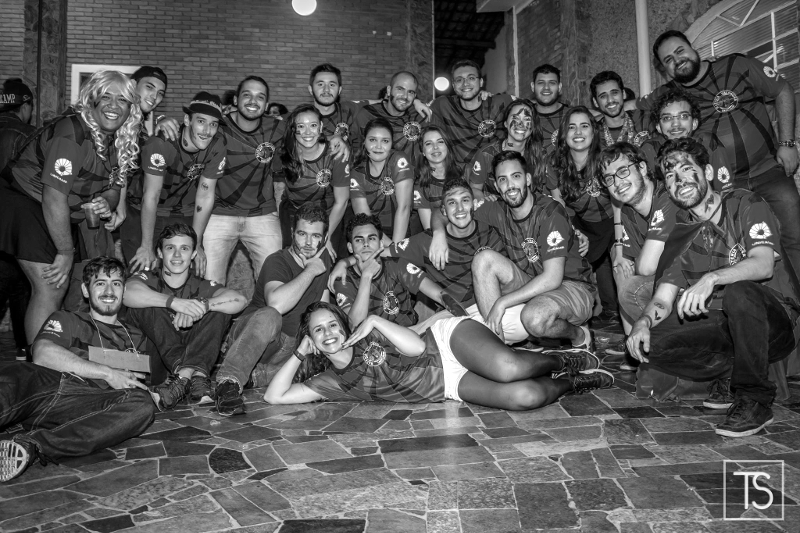
\includegraphics[scale=0.27]{img/alem_da_graduacao/valorosa_foto1.jpg}
\end{figure}

Criada em 1998 e filiada à AAACEC, a \textbf{Bateria Valorosa} é umas das
melhores baterias universitárias da Unicamp. Você muito provavelmente vai
conhecê-la no primeiro dia de aula.

Ao longo do ano, a Valorosa toca em diversos eventos, como o Intercomp, o
Interbatuc e a UPA. A Bateria toca também em festas e para apoiar *s atletas em
jogos internos da Computação e de outros cursos.

A Valorosa realiza ensaios semanais, dos quais estão tod*s, especialmente bix*s,
convidados a participar. Basta comparecer aos ensaios, não é necessário saber
tocar nenhum instrumento. Tod*s que quiserem aprender são muito bem-vind*s na
bateria!

Para mais informações sobre a Bateria Valorosa, acesse o site da AAACEC.

\begin{figure}[H]
    \centering
    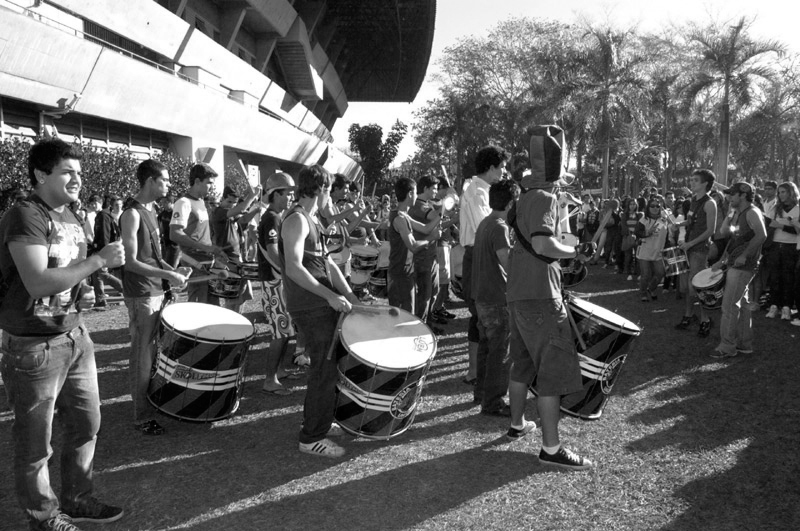
\includegraphics[scale=0.27]{img/alem_da_graduacao/valorosa_foto2.jpg}
\end{figure}

\newpage
%%%%% Bateria Valorosa
% Este arquivo .tex será incluído no arquivo .tex principal. Não é preciso
% declarar nenhum cabeçalho

\section{Bateria Valorosa}

\begin{figure}[H]
    \centering
    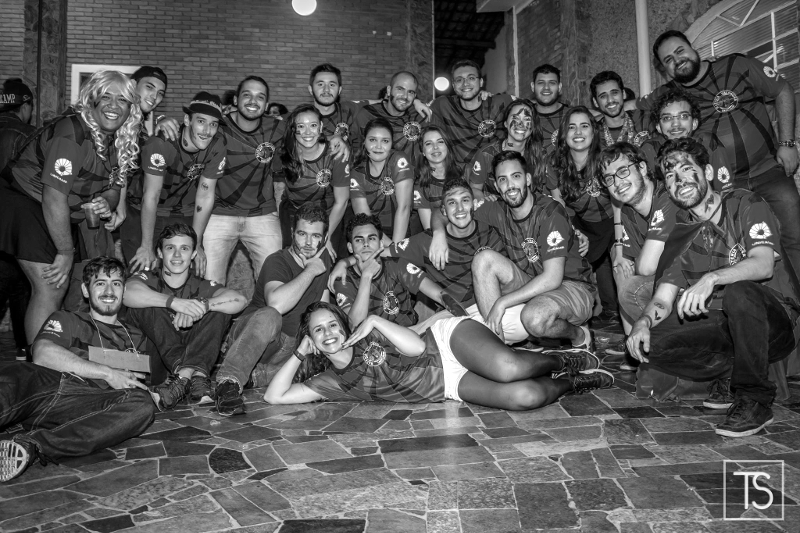
\includegraphics[scale=0.27]{img/alem_da_graduacao/valorosa_foto1.jpg}
\end{figure}

Criada em 1998 por alunos do IC, a \textbf{Bateria Valorosa} é umas das
baterias mais tradicionais da Unicamp, e você muito provavelmente irá
conhecê-la no primeiro dia de aula.

Ao longo do ano, a Valorosa toca em diversos eventos, como o Intercomp, o
Interbatuc e a UPA, além de se apresentar em festas e apoiar as atletas em
jogos internos da Computação e de outros cursos.

A Valorosa realiza ensaios semanais no IC, para os quais estão todas,
especialmente bixetes e bixos, convidadas a participar. Basta comparecer aos
ensaios, não é necessário saber tocar nenhum instrumento. Quem quiser aprender
é sempre muito bem-vinda na bateria!

Para mais informações sobre a Bateria Valorosa, acesse a página no Facebook.
\begin{compactitemize}
\item Facebook: \url{fb.com/bateria.valorosa}
\end{compactitemize}

\begin{figure}[H]
    \centering
    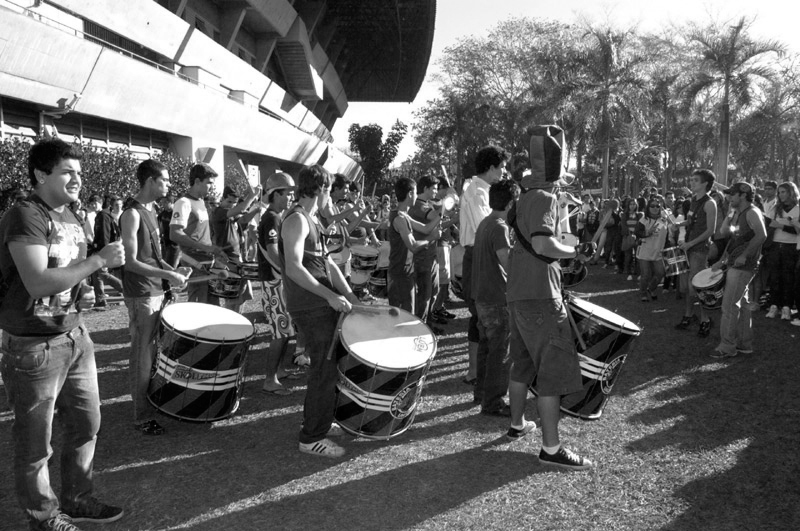
\includegraphics[scale=0.27]{img/alem_da_graduacao/valorosa_foto2.jpg}
\end{figure}

\newpage
%%%%% Conpec
% Este arquivo .tex será incluído no arquivo .tex principal. Não é preciso
% declarar nenhum cabeçalho

\section{Conpec}

\begin{figure}[H]
    \centering
    
\includegraphics[width=.35\textwidth]{img/alem_da_graduacao/conpec_logo.png}
\end{figure}

A Conpec é a empresa júnior dos cursos de Ciência e Engenharia de Computação da
Unicamp.

Nela você tem a oportunidade de aplicar os conhecimentos teóricos adquiridos em
sua vida acadêmica em uma situação real, de mercado, com clientes, prazos e
soluções reais. É uma chance ainda de aprender sobre aspectos de mercado de
trabalho que você nunca veria na faculdade, como marketing, finanças,
planejamento, trabalho em equipe e liderança, indispensáveis considerando-se que
o perfil empreendedor é cada vez mais exigido d* profissional de computação.
Muitos membros e ex-membros da Conpec usam os conhecimentos adquiridos na
empresa não só como um adicional ao buscar uma vaga no mercado de trabalho, mas
também para montar suas próprias empresas ou em serviços não ligados diretamente
à computação, como consultorias estratégicas.

Além disso, a Conpec é uma excelente oportunidade para conhecer *s seus(suas)
colegas de curso, sejam veteran*s ou bix*s, pessoas de outros cursos e até mesmo
de fora da Unicamp, uma vez que há diversas empresas juniores espalhadas pelas
universidades de São Paulo e do Brasil. É ainda uma grande chance para perder a
inibição de falar em público e aperfeiçoar sua capacidade de expor opiniões,
além de aprender como agir em um ambiente profissional.

\begin{figure}[H]
    \centering
    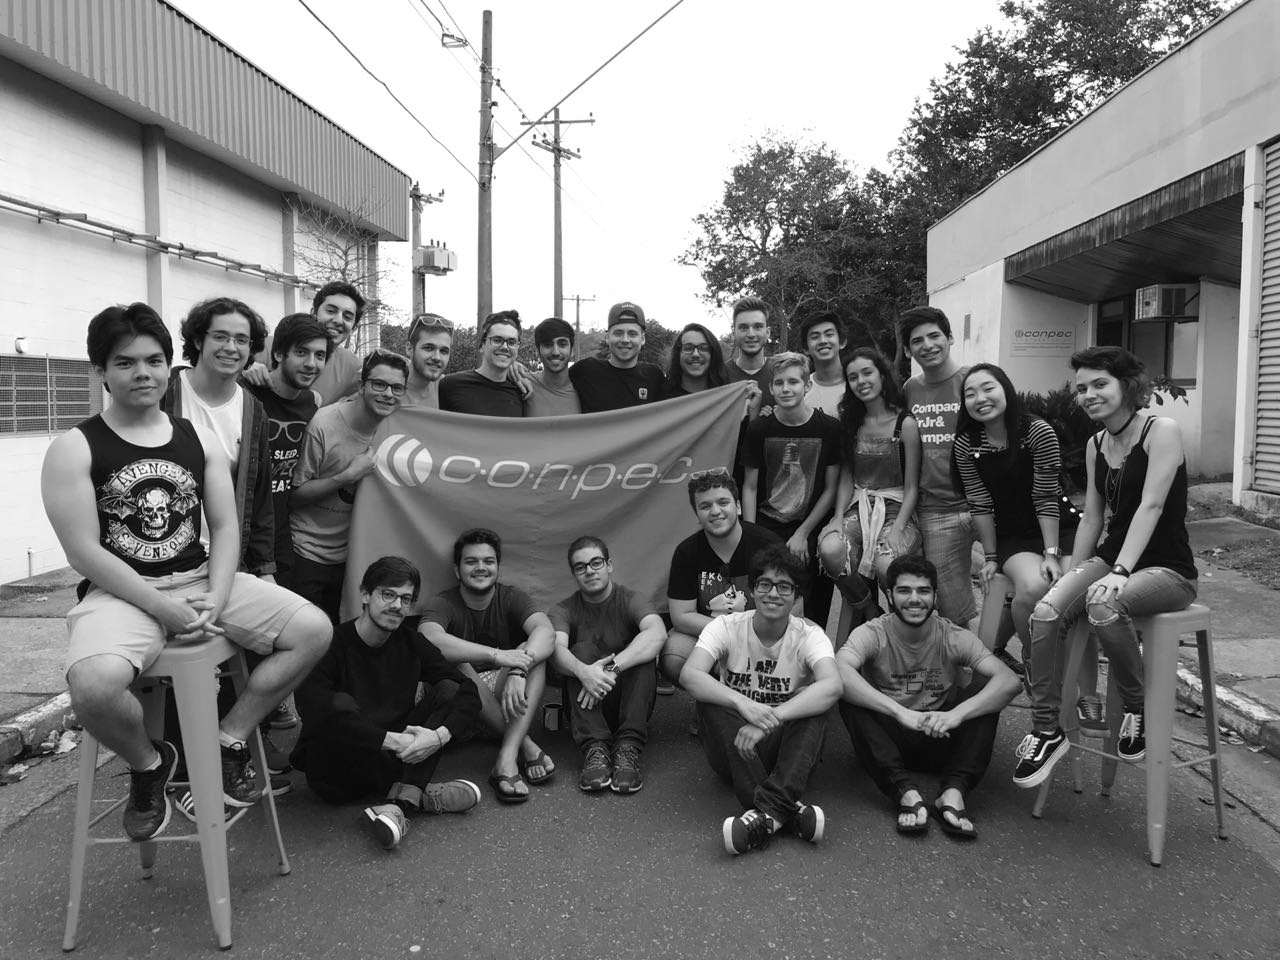
\includegraphics[width=.45\textwidth]{img/alem_da_graduacao/conpec_foto.jpg}
\end{figure}

Para fazer parte da Conpec, fique atent* à data da palestra de apresentação do
processo seletivo, que ocorre no início do ano.

Para saber mais sobre a empresa visite o site \url{conpec.com.br} ou tire suas
dúvidas mandando um e-mail para \email{conpec@conpec.com.br}.

\newpage
%%%%% Computing 4 All
% Este arquivo .tex será incluído no arquivo .tex principal. Não é preciso
% declarar nenhum cabeçalho

\section{Computing 4 All}

O grupo Computing 4 All foi criado para incentivar a diversidade de gênero nos
cursos de computação. Se você está se perguntando o motivo disso ser necessário,
talvez ainda não saiba que há pessoas que deixam de considerar a computação como
uma opção por serem levadas a pensar que essa área requer um perfil bem
específico no qual elas não se encaixam.

Na verdade, a diversidade, seja ela qual for (cultural, religiosa, racial, de
gênero etc.), traz uma grande riqueza para qualquer área e a computação não é
diferente. Por isso, em setembro de 2015, professoras e alunas do Instituto de
Computação decidiram criar um grupo para trabalhar com assuntos relacionados a
esse tema.

Para alcançar a diversidade desejada, o que era a princípio um grupo de mulheres
na computação tornou-se um grupo para tod*s, com o objetivo de incentivar mais
pessoas, independente do gênero, a se interessarem pela área.

\begin{figure}[H]
  \centering
  \includegraphics[width=.24\textwidth]
  {img/alem_da_graduacao/computing4all_logo.png}
\end{figure}

O Computing 4 All realizou em 2015 seu primeiro evento com palestras, painéis e,
em parceria com o CACo, um CineCACo, reunindo professor*s, alun*s e empresas
para comemorar os 200 anos de Ada Lovelace, a pessoa que escreveu o primeiro
algoritmo para ser processado por uma máquina.

Como próximas metas, o grupo pretende realizar projetos, eventos e palestras e
também cursos em parceria com outros grupos da Unicamp para alun*s de ensino
médio e fundamental, com o objetivo de aumentar o interesse pela área através da
exploração do potencial da computação em suas várias facetas.

Se gostou da ideia, venha participar!

% TODO: bit.ly nos links grandes abaixo
\begin{compactitemize}
%\sloppy % Não sei pra que isso serve, não fez diferença (?)
\item Site: \url{computing4all.ic.unicamp.br/}
\item Lista de e-mails: \url{groups.google.com/forum/\#!forum/computing4all}
\item Facebook: \url{fb.com/Computing4All.Unicamp/}
\end{compactitemize}

\newpage
%%%%% Enigma
% Este arquivo .tex será incluído no arquivo .tex principal. Não é preciso
% declarar nenhum cabeçalho

\section{Enigma}

O Enigma é uma entidade formada por alunas e alunos da Unicamp com o propósito
de estudar privacidade, segurança e criptografia, além de outros assuntos
relacionados. Inauguramos nossas atividades com um \textit{Capture the Flag} e
uma palestra na Secomp 2018. Desde então, organizamos encontros, mini cursos,
palestras e desafios para incentivar o desenvolvimento desta área na
universidade.

A área de segurança da informação deixou de ser uma disciplina de nicho para
ser um pré-requisito para todo software que envolve conexão com internet e/ou
dados sensíveis. Todo site e programa pode ser vulnerável, e uma das formas de
aprender a se defender, é aprender o ataque. Por isso, em nossas atividades,
exploramos e discutimos vulnerabilidades, bem como meios de mitigá-las. A
privacidade é um direito fundamental do ser humano e que garante um
funcionamento democrático da sociedade. Esse direito tem sido cada vez mais
negligenciado na era digital, com abusos por parte de corporações e governos.
Através da criptografia é possível transmitir e armazenar dados de forma
segura e garantida que somente aqueles com os devidos poderes podem vir a
acessá-los, sendo uma ferramenta essencial tanto para privacidade quanto para a
segurança.

Todas as pessoas são bem vindas, independentemente do seu curso e experiência
prévia! Somos abertos, sem processo seletivo ou hierarquias e acreditamos que
o conhecimento deve ser livre.

\begin{figure}[H]
  \centering
  
\includegraphics[width=.24\textwidth]
  {img/alem_da_graduacao/enigma_logo.jpg}
\end{figure}


\begin{compactitemize}
\item Site: \url{enigma.ic.unicamp.br/}
\item Email: \url{enigmaunicamp@tutanota.com}
\item Grupo do Telegram: \url{https://t.me/enigmaunicamp}
\end{compactitemize}

\newpage
%%%%% Grupos e Entidades da Unicamp
% Este arquivo .tex será incluído no arquivo .tex principal. Não é preciso
% declarar nenhum cabeçalho

\section{Grupos e Entidades da Unicamp}

\subsection{Alumni Computação Unicamp}

\begin{figure}[H]
  \centering
  \includegraphics[width=.35\textwidth]{img/alem_da_graduacao/alumni_logo.png}
\end{figure}

Alumni é o nome dado a ex-alunas e ex-alunos de uma universidade. Por extensão,
alumni também é o nome de organizações sem fins lucrativos motivadas em manter
o relacionamento entre a universidade e os ex-alunas(os) e o destes entre si,
servindo como uma rede de contatos profissionais. A comunicação entre alunas,
alunos, ex-alunas, ex-alunos, professoras e professores proporciona um
compartilhamento de experiência e informações, que contribuem para uma
diferenciação acadêmica, cultural e profissional.

O \textbf{Alumni Computação Unicamp} é uma forma de manter todas e todos que
passaram pelo melhor curso de computação da América Latina conectados -- tanto
alunas e alunos quanto ex-alunas e ex-alunos. Atualmente o Alumni conta com uma
página no Facebook \\(\url{fb.com/AlumniComputacaoUnicamp}), que reúne\\os
grupos das turmas que passaram pela Computação, com o objetivo de atingir o
maior número de participantes.

Participe do grupo de sua turma, convide seus amigos a curtirem a página, envie
sugestões e contribua para essa ideia!

\subsection{ARU -- Associação de Repúblicas da Unicamp}

\subsubsection{O que é a ARU?}

\begin{figure}[H]
  \centering
  \includegraphics[width=.35\textwidth]{img/alem_da_graduacao/aru_logo.png}
\end{figure}

Idealizada em 2008, a ARU é a entidade que representa as Repúblicas Associadas
de Barão Geraldo. Tem como meta prestar apoio a elas, zelar pela sua segurança
e bem estar com toda a vizinhança, como também servir de espaço para discutir
os problemas apresentados em reuniões.

\begin{figure}[H]
  \centering
  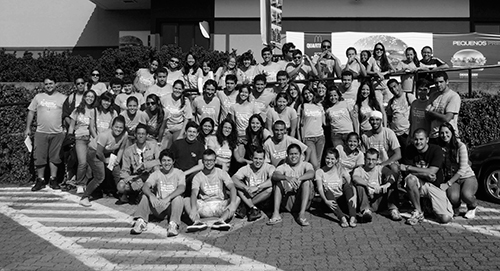
\includegraphics[width=.45\textwidth]{img/alem_da_graduacao/aru_foto.jpg}
\end{figure}

Além de entregar no começo do ano um manual para as bixetes e para os bixos,
contendo informações sobre as Repúblicas Associadas, a ARU também realiza
vários eventos, os quais têm o objetivo de integrar e divertir as moradoras e
moradores de repúblicas. Alguns deles são: a \textbf{Alcorrida}, a
\textbf{Campanha do Agasalho}, o \textbf{EntortaRep}, e, principalmente, o
\textbf{InterReps}.

\subsubsection{Contato}

\begin{compactitemize}
\item Site: \url{republicasunicamp.com.br}
\item E-mail: \email{contato@republicasunicamp.com.br}
\item Facebook: \url{fb.com/republicasunicamp}
\end{compactitemize}

\subsection{Competições de programação}

Curte programar? Nunca programou, mas está gostando de MC102? Já brincou de
Olimpíada naquelas provas com direito a medalha? Vá fundo!

Para as bixetes e bixos que ingressaram direto do ensino médio existe a
\textbf{OBI --Olimpíada Brasileira de Informática}, logo no primeiro semestre.
Anualmente, muitas alunas e alunos do IC, tanto da ciência como da engenharia,
ganham premiações nessa competição. O site dela é
\url{olimpiada.ic.unicamp.br}. Visite-o para mais informações.

\begin{figure}[h!]
  \centering
  \includegraphics[width=.35\textwidth]
  {img/alem_da_graduacao/maratona_logo.png}
\end{figure}

Mas a principal competição para alunas e alunos de ensino superior é a
\textbf{Maratona de Programação}, que consiste de problemas mais difíceis e é
feita em equipes de três alunas(os). A Unicamp tem grande tradição nessa
competição, tendo levado equipes para a competição mundial (a ACM-ICPC) em
1996, 2000, 2002, 2003, 2004, 2007, 2009, 2012, 2013, 2014, 2015, 2016 e vamos
levar em 2018!

Além de brilhar no currículo, é muito divertido competir e a experiência obtida
nos treinamentos tem levado muitas(os) maratonistas a empresas como Google,
Microsoft e Facebook.

Para participar dos treinamentos para a Maratona que acontecem na Unicamp,
visite a wiki \url{www.ic.unicamp.br/~maratona/wiki}.

\subsection{Gamux}

\begin{figure}[h!]
  \centering
  \includegraphics[width=.2\textwidth]{img/alem_da_graduacao/gamux_logo.png}
\end{figure}

O \textbf{Gamux} (Grupo de Pesquisa e Desenvolvimen\-to de Jogos da Unicamp),
composto por computeiras, computeiros, alunas e alunos do IA (Instituto de
Artes), é uma ótima oportunidade para quem tiver curiosidade de saber como são
feitos os jogos eletrônicos.

Costumam organizar aulas de introdução ao desenvolvimento de jogos para as
bixetes e bixos, além de ciclos de palestras e eventos ao longo do ano para a
confecção de jogos.

Fique atenta: acesse o site, a página do Facebook ou o grupo de e-mail para se
manter informado e saber mais sobre o Gamux:

\begin{compactitemize}
\item Site: \url{gamux.com.br}
\item Facebook: \url{fb.com/gamux}
\item Lista de discussão: \url {bit.ly/1AplfKK}
\end{compactitemize}

\subsection{DCE -- Diretório Central dos Estudantes}

Criado em 1978, o DCE Unicamp (Diretório Central dos Estudantes) é a entidade
que representa estudantes de graduação da Universidade, articulando e
organizando o movimento estudantil (ME).

Cabe ao DCE representar o conjunto de estudantes em todos os espaços dentro e
fora da universidade, diante das mais diversas entidades (reitoria, sindicatos,
DCEs de outras universidades, centros acadêmicos, associações etc.) e
movimentos sociais.

Como articulador do ME, cabe ao DCE organizar estudantes na luta por uma
educação superior realmente pública, gratuita e de qualidade. Para tanto, é
papel fundamental do DCE propor, juntamente com os centros acadêmicos,
discussões políticas que extrapolem os nossos currículos e o nosso dia a dia.
Além disso, o DCE deve propor ações que vão ao encontro das reivindicações
estudantis, de forma que elas sejam levadas e cobradas da reitoria ou até mesmo
do governo.

O DCE esteve envolvido em várias conquistas dos estudantes, das quais se
destacam algumas lutas históricas: a construção da moradia estudantil; a
melhoria de estrutura para cursos noturnos, que tornou acessível para esse
período bibliotecas, xerox, laboratórios e secretarias de graduação; a reunião
semestral para avaliação de curso; o não aumento drástico do preço do bandejão;
uma seleção mais justa para as vagas na moradia; entre diversas outras. Além
disso, o DCE teve participação em importantes lutas sociais que extrapolam o
âmbito da Unicamp, como a organização do Plebiscito contra a Alca e do
Plebiscito contra o Provão; a luta por mais verbas para a educação no estado de
São Paulo; diversas lutas pela qualidade do ensino e manutenção de direitos dos
estudantes em outras universidades como na UNIP, UNIMEP, FUPPESP etc.

No fim do ano, há eleições para definir qual a chapa que comandará a entidade
no ano seguinte, juntamente com eleições para representação discente no Consu e
na CCG. É muito importante a participação de alunas e alunos nessas eleições,
então estejam sempre ligadas(os) durante o ano inteiro sobre as atividades do
DCE: estão cumprindo o programa da chapa? As atividades estão atendendo às
demandas estudantis? Integrantes da chapa do DCE estão dialogando com
estudantes e com as entidades estudantis? Estejam sempre antenadas(os) para que
nossos representantes no DCE permaneçam atendando aos interesses de estudantes,
pois assim podemos continuar os avanços dentro da nossa universidade.

Além disso, o DCE organiza a Calourada Integrada juntamente com os centros
acadêmicos. Elas que acontecem na sede do DCE, próxima ao Bandejão. Não deixe
de participar!

\begin{compactitemize}
\item Telefone: (19) 3521-7910 / (19) 3521-7042
\item E-mail: \email{dceunicamp@gmail.com}
\end{compactitemize}

\subsection{Equipe Phoenix}

\begin{figure}[h!]
  \centering
  \includegraphics[width=.35\textwidth]{img/alem_da_graduacao/phoenix_logo.png}
\end{figure}

A Equipe Phoenix de Robótica da Unicamp é composta por alunos da Mecânica,
Elétrica e Computação, e desenvolve projetos todo ano para participar de
competições nacionais como a RoboCore, disputando pela categoria de melhor robô
de combate, sumô, trekking e seguidor de linha, entre outros.

Para interessadas e interessados pela programação de um robô,  pela eletrônica
das placas de controle ou ainda pela mecânica dos robôs que resistem a impactos
gigantescos durante a guerra, a equipe realiza um processo seletivo todo começo
de ano, com inscrições através do site. Se envolva!

\begin{compactitemize}
\item Site: \url{phoenixunicamp.com.br}
\item Facebook: \url{fb.com/phoenixunicamp}
\end{compactitemize}

\subsection{GER -- Grupo de Estudos em Robótica}

\begin{figure}[h!]
    \centering
    \includegraphics[width=.35\textwidth]{img/alem_da_graduacao/ger_logo.jpg}
\end{figure}

O GER – Grupo de Estudos em Robótica – é uma entidade extra-curricular
associada à Faculdade de Engenharia Mecânica (FEM) da Universidade Estadual
de Campinas (Unicamp). Criado e formado por alunos da Unicamp, o GER tem por
objetivos aprender, sobre robótica, programação, eletrônica e áreas afins,
aplicando, na prática, os conhecimentos adquiridos ao longo da graduação,
além de compartilhar e trocar conhecimentos com a comunidade. Para isso,
desenvolvemos projetos como Seguidor de Pista, Futebol de Robôs, SEK, Corrida
de Humanoides, Drone, Cursos, Social. Atualmente, contamos com alunos de
diversos cursos, como engenharia mecânica, de controle e automação, elétrica,
de computação e ciência da computação.

\begin{compactitemize}
\item Site: \url{gerunicamp.com.br}
\item E-mail: \email{contato@gerunicamp.com.br}
\end{compactitemize}


\subsection{Startup Lab}

\begin{figure}[h!]
  \centering
  \includegraphics[width=.35\textwidth]
  {img/alem_da_graduacao/startup_lab_logo.png}
\end{figure}

Antes de tudo: O que é uma startup?

Startup significa o ato de começar algo, normalmente relacionado com companhias
e empresas que estão no início de suas atividades e que buscam inovar o
mercado. O Startup Lab Unicamp quer orientar empreendedoras e empreendedores
universitários e startups em suas fases embrionárias afim de apoiá-las em seu
desenvolvimento até alcançarem seu potencial a ponto de se tornarem grandes
empresas. Quer aprender a transformar uma ideia em algo real? Venha nos
conhecer!

\begin{compactitemize}
\item Site: \url{fb.com/UnicampStartupLab}
\end{compactitemize}


\subsection{LibrePlanet São Paulo}

\begin{figure}[h!]
  \centering
  \includegraphics[width=.45\textwidth]
  {img/alem_da_graduacao/lp-br-sp-logo.jpg}
\end{figure}

Numa sociedade controlada majoritariamente por algoritmos e com nossos dados
pessoais fluindo livremente pela Internet, surge a necessidade de lidar com
questões éticas, em especial, responder a pergunta: Quem realmente controla os
programas que você usa?  O movimento do \textbf{Software Livre} busca resolver
este dilema ético, devolvendo o controle do computador aos usuários, de forma
que estes possam recuperar sua privacidade e o controle sobre sua computação.

O \textbf{LibrePlanet São Paulo} é um grupo dedicado a discutir as questões que
permeiam a filosofia do Software Livre, como liberdade, \emph{hacking},
segurança e privacidade vs. vigilância estatal. Uma parte importante do nosso
ativismo é ensinar as pessoas a reconhecerem armadilhas proprietárias na
computação. Essas armadilhas podem estar tanto em programas de computador que
executam localmente na sua máquina, quanto em serviços online que invadem nossa
privacidade e nos forçam a utilizar tecnologias prejudiciais à liberdade. Por
isso, além de colocarmos bastante ênfase na divulgação de\\Softwares Livres,
também oferecemos alguns serviços pela internet que podem ajudar os usuários a
se livrarem dessa dependência nociva.

Desde 2013, O LibrePlanet organiza o \textbf{Curso de GNU/Linux para os Bixos}.
Este curso, como o próprio nome diz, é voltado para as bixetes como você e
bixos que ingressam nos cursos de computação, embora seja aberto também a
veteranas e veteranos. O objetivo é o ensinar o básico do sistema operacional
GNU/Linux para você começar a se virar no resto da graduação. O curso acontece
nas primeiras semanas de aula, mas não se preocupe, você será avisada na sala
de aula por alguma veterana ou algum veterano, além de receber um comunicado
pelo seu e-mail do IC.

Não perca também a oportunidade de instalar o Sistema Operacional GNU/Linux no
seu computador durante o \textbf{Installfest} organizado pelo LP. O
conhecimento sobre esse sistema será extremamente útil para a sua vida como
computeira ou computeiro, não só durante a faculdade!

\begin{compactitemize}
\item Site: \url{libreplanetbr.org}
\item E-mail: \email{libreplanet-br-sp@libreplanet.org}
\end{compactitemize}

\subsection{MTE -- Mercado de Trabalho em Engenharia}

\begin{figure}[h!]
  \centering
  \includegraphics[width=.35\textwidth]{img/alem_da_graduacao/mte_logo.png}
\end{figure}

O \textbf{MTE -- Mercado de Trabalho em Engenharia} é uma entidade estudantil
que visa colocar a aluna ou aluno da Unicamp em contato mais próximo com o
mercado de trabalho e com as possibilidades que ele proporciona, mostrando as
diferentes áreas de atuação de uma engenheira ou engenheiro.

A participação no MTE desenvolve habilidades como networking, oratória,
expressão, empreendedorismo, gestão e diversas outras.

A estrutura do MTE é dividida em três pilares:

\begin{description}
\item[Oportunidades:] responsável por atividades co\-mo visitas técnicas e
  captação de treinamentos e palestras.

\item[Desenvolvimento:] responsável por atividades co\-mo English Meeting
  (encontros de conversação em inglês), Teia do Conhecimento (treinamentos
  dados por algum dos membros) e Ciclo de Oratória (ciclos com foco em melhoria
  de expressão).

\item[Orientação e Carreira:] responsável pela estruturação pessoal e
  profissional dos membros realizando feedbacks, atividades de consultoria, de
  motivação, entrevista com profissionais e confraternizações.
\end{description}

Além da participação em um dos pilares, alguns membros participam da diretoria
administrativo-financeira e, para completar, participam da realização de dois
principais eventos: o EMC (Estudante e Mercado Conectados) que conta com
visitas técnicas e palestras e o ArenaMTE, um desafio universitário de
resolução de cases.

Para mais informações sobre o MTE e seu processo seletivo, acesse
\url{mte.org.br}.

\subsection{Rádio Muda}

Você provavelmente nunca viu nada do tipo na sua vida. Uma rádio na qual
qualquer ser humano pode fazer o seu programa tranquilamente, sem burocracias
(tendo espaço na grade de horários, lógico).

A Rádio Muda fica embaixo da caixa d'água (carinhosamente apelidada de Pau do
Zeferino) que fica perto do Teatro de Arena, bem em frente à BC (Biblioteca
Central).

Se você só quiser ouvir a muda, 88,5 MHz no seu rádio (em Barão Geraldo ou
Paulínia) ou pela Internet, através do site \url{muda.radiolivre.org}.

\subsection{Curso Exato}

O Curso Exato é um projeto da Pró-Reitoria de Extensão e Assuntos Comunitários
da Unicamp criado em 2008 por alunas e alunos de graduação, com a finalidade de
explorar o potencial e a capacidade de alunas(os) de se expressarem, de
raciocinarem logicamente e de compreenderem o mundo que as(os) cerca, por meio
de aulas de língua portuguesa, matemática, física e química.

As professoras e professores do curso são alunas e alunos de graduação e
pós-graduação da universidade e o público alvo é constituído por alunas e
alunos da rede pública de ensino com disposição e interesse para aprender.

As aulas são realizadas no período noturno, das 19h15 às 22h30, de segunda a
quinta-feira, no campus da universidade.

\begin{compactitemize}
\item Site: \url{bit.ly/1GajCZS}
\item Facebook: \url{fb.com/curso.exato}
\item E-mail: \email{curso.exato@gmail.com}
\end{compactitemize}

\subsection{Grupos Religiosos}

\subsubsection{ABU -- Aliança Bíblica Universitária}
% Há vários links, sites e páginas no Facebook, não sei qual colocar pois não
% conheço a relação entre eles. Se alguém puder, complete.

Grupo evangélico não ligado a nenhuma denominação, organiza várias reuniões e
grupos de discussões e é filiado à Aliança Bíblica Universitária do Brasil
(\url{abucampinas.blogspot.com.br}).

\begin{compactitemize}
%\item Site: \url{abucampinas.org}
\item E-mail: \email{contato@abucampinas.org} ou
  \email{abucamp_co@yahoogrupos.com.br}
\item Telefone: (19) 3289-2823
\end{compactitemize}

\subsubsection{Pastoral Universitária}

Grupo católico que se reúne semanalmente para estudar textos (bíblicos ou não),
livros, documentos, aprofundar a fé e promover a integração e união de seus
participantes. A Pastoral Universitária também organiza grupos de preparação
para Primeira Comunhão e Crisma, além de duas Missas semanais e Grupos de
Oração Universitários (GOUs). As Missas são realizadas às terças (18h) e às
quintas (12h15), sempre no PB04. Os GOUs acontecem às terças (12h15) e nas
quintas (18h), também no PB04.

\begin{compactitemize}
\item Site:
\begin{small}
  \url{sites.google.com/site/pastoralunicamp}
\end{small}
\item E-mail: \email{pastoralunicamp@gmail.com}
\end{compactitemize}

\newpage
%%%% Eventos da Unicamp
% Este arquivo .tex será incluído no arquivo .tex principal. Não é preciso
% declarar nenhum cabeçalho

\section{Eventos da Unicamp}
\subsection{Feira do Livro}

Evento iniciado em 2002, a cada dois anos a Editora da Unicamp realiza a Feira
do Livro, no Ginásio da Unicamp. Há excelentes opções, de diversas editoras,
principalmente na área de literatura, artes e humanas, com no mínimo 50\% de
desconto.

\subsection{Semanas da Unicamp}

Alguns cursos da Unicamp realizam anualmen\-te um evento (chamado de Semana) em
que as alunas e alunos de graduação têm um contato com o mercado de trabalho,
com as pesquisas, com as tendências e novidades dos cursos e demais assuntos,
ramos e áreas de cada curso. Para isso, participam desse evento ex-alunas,
ex-alunos e profissionais, realizam-se palestras e minicursos, são feitas
visitas a empresas e debates (mesas redondas).

\subsubsection{Secomp -- Semana da Computação}

\begin{figure}[H]
  \centering
  \includegraphics[width=.35\textwidth]{img/alem_da_graduacao/secomp_logo.png}
\end{figure}

A computação tem a sua própria semana, organizada pela entidade de mesmo nome,
com ajuda de membros das três entidades estudantis: CACo, AAACEC e Conpec. O
evento busca aproximar e relacionar os três pilares da graduação: estudantes, a
universidade e o mercado. Dessa forma, a Secomp -- Semana da Computação --
procura mostrar às alunas e aos alunos a diversidade de caminhos a seguir e um
pouco do que cada área pode oferecer.

Durante seus sete dias de duração, a Semana traz uma gama de atividades, entre
palestras, oficinas, cursos, visitações e outros eventos, para que
participantes possam ter uma visão abrangente do mercado e da própria
universidade. Além disso, a Secomp tem atividades voltadas ao recrutamento em
grandes empresas, para aqueles à procura de vagas.

Você pode achar que nada disso importa ainda, bixete, mas não tem problema. A
Semana também tem uma fartura -- literalmente -- de coffee-breaks, brindes e
prêmios sorteados. Tudo isso pago pelo IC para você, então não perca!

Para saber mais sobre o evento, é só acessar a página da Secomp
(\url{secomp.com.br}).

\subsection{Talento}

Talento é um evento que acontece todo ano, des\-de 1999, durante um dia
inteiro, no Ginásio Multidisciplinar e organizado pelo Núcleo de Empresas
Juniores da Unicamp. Trata-se de uma feira de recrutamento, onde alunas e
alunos da Unicamp e de outras universidades e o público em geral têm contato
com empresas, seja por meio de palestras, mesas redondas e estandes, e estas
apresentam o seu processo seletivo. Nesse evento também é feito o cadastro de
currículos dos visitantes.

Para saber mais sobre o evento, é só acessar a página da Talento
(\url{talentounicamp.com.br}). O evento é gratuito.

\subsection{UPA -- Unicamp de Portas Abertas}

\begin{figure}[h!]
  \centering
  \includegraphics[width=.45\textwidth]{img/alem_da_graduacao/bateria_upa.jpg}
\end{figure}

A \textbf{UPA} é um evento anual em que, durante um dia, agora no primeiro
semestre, a Unicamp é apresentada para estudantes dos ensinos fundamental e
médio de todo o país, muitos dos quais pré-vestibulandas e pré-vestibulandos. A
apresentação da universidade é feita por professoras, professores, alunas e
alunos, que mostram as salas de aula e as pesquisas realizadas.

No ano de 2014, a UPA recebeu a visita de 42 mil alunas e alunos de 654 escolas
públicas e privadas originárias de vários estados do Brasil.

O IC costuma realizar uma recepção com forte participação das alunas e dos
alunos. Se você é como toda bixete ou bixo e está louca para pagar de estudante
da Unicamp, esta é uma oportunidade excelente! Além de ser divertido, o IC
geralmente oferece uma pequena remuneração pelo trabalho. Participe!

Para saber mais sobre o evento, é só acessar a página \url{www.upa.unicamp.br}.

\newpage
%%%%% Serviços da Unicamp
% Este arquivo .tex será incluído no arquivo .tex principal. Não é preciso
% declarar nenhum cabeçalho

\section{Serviços da Unicamp}
\subsection{Atendimento médico e odontológico -- CECOM}

A CSS é responsável pelo planejamento e execução de programas de saúde voltados
à comunidade universitária da Unicamp -- alun*s, funcionári*s e docentes. É
responsável também pelo atendimento à saúde oral desta comunidade, incluindo
também *s filh*s menores de servidor*s que estejam devidamente matriculados nas
creches e escolas dos campi.

Em português, isso quer dizer que é um ``plano de saúde'' da Unicamp. Demora um
pouco (embora o pronto-socorro do CECOM seja bem mais rápido que o do HC), tem
burocracia, mas funciona. Você pode marcar consultas médicas e fazer exames. O
CECOM é localizado próximo ao HC. Para ir, é melhor pegar o Circular pois é
beeeeeem longe. De circular interno, peça para descer no CECOM. É o ponto final
ou o penúltimo dos circulares.

Fique de olho na sua caixa de entrada perto do período de inverno, pois o CECOM
costuma disponibilizar vacina contra gripe gratuitamente, uma dose em clínica
particular é bem cara, vale a pena.

Caso você tenha Unimed, o Centro Médico, que fica perto da Unicamp, atende pela
Unimed. É mais rápido que o atendimento da Unicamp (CECOM ou SUS).

%%% Imagem do hospital
\begin{figure}[h!]
    \centering
    \includegraphics[width=.45\textwidth]{img/alem_da_graduacao/hc.jpg}
    \caption{Vista do Hospital de Clínicas da Unicamp}
\end{figure}

Para marcar consultas com Dentista, vá ao CECOM e pergunte onde que é. Isso é
mais fácil que você tentar entender lendo aqui. Basicamente é embaixo do CECOM,
muito fácil de chegar se alguém apontar com e dedo e dizer ``ali''. Funciona
muito bem, o atendimento é ótimo. A única burocracia é assistir uma palestra
sobre doenças da boca e escovação antes de poder marcar atendimento. Mas se
você estiver com dores el*s te atendem na hora sem marcar consulta nem assistir
palestra.

Para saber mais sobre o CECOM, vá ao site deles (\url{www.cecom.unicamp.br}).

\subsection{Hemocentro}

Essa é para quem é (ou para quem quer ser) doador(a) de sangue. O centro de
hematologia e hemoterapia (Hemocentro) é o órgão da Unicamp responsável pela
coleta e doação de sangue.
\begin{wrapfigure}{r}{.2\textwidth}
    \centering
    \includegraphics[width=.2\textwidth]{img/alem_da_graduacao/doe_sangue.jpg}
\end{wrapfigure}
Qualquer pessoa pode aparecer no Hemocentro para fazer a doação de sangue.
Basta estar com o RG e seguir um conjunto de normas para a doação de sangue.
Para saber mais sobre o processo, é só visitar a página do Hemocentro
(\url{www.hemocentro.unicamp.br}).

O Hemocentro também faz o projeto doador(a) universitári*, que consiste de
unidades móveis (ônibus) que param em alguns pontos do campus. Essas unidades
fazem a coleta do sangue. Alun*s, professor*s e funcionári*s podem ir até essas
unidades móveis para fazer a doação. Para se informar melhor, é só visitar a
página do projeto: \url{bit.ly/14xaTAn}.

O Hemocentro fica localizado acima do HC (próxima ao CECOM). Portanto, se
quiser se deslocar até lá, como está escrito acima, é melhor usar o circular
interno.

\subsection{Circular Interno e Ônibus Moradia}

\subsubsection{Circular Interno}
É um serviço de ônibus gratuito que dá voltas na Unicamp. Há duas linhas, uma
girando no sentido horário e outra no anti-horário.  Só funciona até às
19h20min, e a frequência maior é no horário de almoço. Bom para cobrir
percursos como bandejão ao IC, IC à FEEC, qualquer lugar ao CECOM, qualquer
lugar à FEAGRI, FEAGRI à qualquer lugar. Quase todos os pontos têm os
itinerários e os horários afixados, além de também estarem disponíveis no
aplicativo da ``Unicamp Serviços'' para celular. Ele não costuma atrasar nem
adiantar mais que 5 minutos, exceto no período de férias.

\subsubsection{Circular Noturno}
É um ônibus que dá uma volta na Unicamp partindo do balão da Avenida 1, passando
pela BC, IQ, FEEC, IC e voltando para o balão da Avenida 1. Os horários e o
itinerário desse ônibus também estão no aplicativo e em alguns pontos como os
do Circular Interno 1 e do 2. Ele funciona das 18h às 23h, a cada meia hora.

\subsubsection{Ônibus Moradia}
Também conhecido como ``Circular Externo'', ele faz o trajeto da Unicamp,
partindo do estacionamento da BC, para a Moradia e o trajeto contrário. Alguns
ônibus, a partir das 18h dão uma volta na Unicamp antes de ir para a
Moradia. Outros fazem rotas alternativas em horários específicos que cobrem as
regiões da Avenida 1, Centro de Barão Geraldo e Avenida 3. Os horários mais
lotados do Ônibus Moradia são 8 da manhã (sentido Moradia--Unicamp), horário de
almoço (ambos os sentidos), horário de jantar (ambos os sentidos) e o último
horário (Unicamp--Moradia). Se puder evitar esses horários, faça-o.

Todos os itinerários e horários detalhados dos serviços de ônibus podem ser
encontrados na página da Prefeitura da Unicamp: \\\url{prefeitura.unicamp.br}.
Você também consegue acessá-los a partir do aplicativo ``Unicamp Serviços'',
disponível pra Android e iOS.

\subsection{SAE -- Serviço de Apoio ao Estudante}
\begin{wrapfigure}{l}{.2\textwidth}
%\begin{figure}[h!]
    \centering
    \includegraphics[width=.2\textwidth]{img/alem_da_graduacao/sae.jpg}
%\end{figure}
\end{wrapfigure}
O SAE (Serviço de Apoio ao Estudante), principal órgão de apoio ao estudante na
Unicamp, atua em várias frentes de assistência estudantil. Esta se dá por meio
do gerenciamento de bolsas-auxílio, assistência social e orientações
educacional, jurídica e psicológica, além de apoio a projetos acadêmicos e
sociais e programa de intercâmbio de estudantes no exterior. O SAE também é
responsável pela gestão de estágios na Universidade.

\begin{itemize}
    \item  Localização: Prédio do Ciclo Básico, 3º piso (responsável pelo
        gerenciamento de convênios, estágios, bolsa-pesquisa e bolsa-empresa);
        e ao lado da cantina do DCE (serviço social, responsável pelo
        gerenciamento de bolsas-auxílio).
    \item  Horário: Segunda a sexta, das 08h30 às 20h, no período letivo.
    \item  Contato: \email{sae@unicamp.br}
    \item  Site: \url{www.sae.unicamp.br}
\end{itemize}

\subsection{Bolsas-Auxílio}
\subsubsection{Moradia}

Criado em 1989, o Conjunto Residencial Universitário da Unicamp, tem por
finalidade garantir estadia gratuita e de qualidade para *s estudantes que
passam por dificuldades sócio-econômicas.

Para saber mais sobre o processo seletivo entre no site da Moradia da Unicamp
(\url{www.pme.unicamp.br}).

\subsubsection{Bolsa Alimentação e Transporte}

Objetivo: Colaborar com * estudante de graduação e pós-graduação em dificuldade
sócio-econômica, nos itens alimentação e transporte.

Critérios para a seleção: Análise do questionário sócio-econômico devidamente
preenchido e documentado, e entrevista com a assistente social.

\subsubsection{Bolsa Trabalho}

Objetivo: Colaborar com o estudante de graduação em dificuldade
sócio-econômica, cuja família não tenha condições de mantê-lo na Universidade.
Em contrapartida * bolsista trabalhará 15 horas semanais em unidades da
Unicamp, ou em grupos de pesquisas, ou em grupos sociais, em horário compatível
com o horário escolar. E com a orientação de um(a) professor(a).

Critérios para a seleção: Análise do questionário sócio-econômico devidamente
preenchido e documentado, e entrevista com a assistente social.

Alun*s da pós não podem se candidatar à bolsa trabalho.

\subsubsection{Bolsa Emergência}

Objetivo: Atender *s estudantes de graduação regularmente matriculad*s que
estejam passando por dificuldades econômicas emergenciais. Em contrapartida o
bolsista trabalhará 40 horas em unidades da Unicamp, compatível com o horário
escolar.

Procedimento: * candidat* deverá enviar uma carta à Coordenação do SAE
solicitando o benefício e informando sobre os motivos. Preencher e entregar
devidamente documentado o questionário sócio-econômico e marcar entrevista com
a assistente social.

Critérios para seleção: Análise da solicitação, do questionário sócio-econômico
devidamente preenchido, documentado e entrevista com a assistente social.

Alun*s da pós não podem se candidatar à bolsa emergência.

\subsubsection{Bolsa PAPI}

Busca incentivar a participação de alun*s de graduação e de pós-graduação nas
mais diversas atividades da Unicamp, tais como no auxílio a eventos. Neste
programa, há a solicitação de estudantes por parte de alguma Unidade ou órgão
da Unicamp, que poderá indicar o nome d* alun* ou deixar a critério do SAE para
fazê-lo.

\subsection{Assistência Jurídica}

Objetivo: Orientar *s alun*s nacionais ou estrangeiros de graduação ou
pós-graduação, na resolução de suas questões pessoais de cunho jurídico que
envolvam os ramos do Direito, principalmente os seguintes:

\begin{description}
    \item[Direito Civil:] Contratos em geral; contratos de locação de
        imóvel/escritura de compromisso de venda e compra; acidentes de
        trânsito; reparação de dano; ação revisional de aluguel; separação
        judicial; divórcio; pensão alimentícia, etc.

    \item[Direito Penal:] Violência contra a pessoa; lesões corporais; furto;
        roubo etc{\dots}

    \item[Direito do Trabalho:] Caracterização de relação de emprego para *s
    não registrados e direitos trabalhistas em geral (normas da CLT).
\end{description}

Procedimento: * alun* deve dirigir-se pessoalmente ao SAE para obter os
esclarecimentos desejados.

Delitos de consumo, encaminhar ao SEDECON ou ao PROCON.

Com relação aos contratos de locação alertamos para algumas dicas importantes:

\begin{itemize}
    \item  Jamais pagar qualquer valor antecipadamente (ex: ``taxas de reserva
        de imóvel'', ``taxa de contrato'', aluguel antecipado etc), ou fornecer
        títulos em garantia: cheque pré-datado, nota promissória.

    \item  Obter o maior número de informações possíveis relativas ao imóvel,
        proprietári*(s), imobiliária, procuradores;

    \item  Condições e valores para pagamento (aluguel e outros encargos ex.:
        Condomínio, IPTU, seguros etc, para uma real visualização do valor
        total a ser despendido).

    \item  Sempre solicitar uma Minuta do contrato locação.

    \item  Não assinar contrato ou qualquer outro documento antes de
        apresentá-lo para análise por um dos advogados da O.J. SAE.
\end{itemize}

\subsection{Orientação psicológica}

Objetivo: Prestar atendimento psicológico ao estudante de graduação,
pós-graduação e especial.

O Serviço de Orientação Psicológica do SAE funciona em associação com o Serviço
de Atendimento Psicológico e Psiquiátrico ao Estudante (SAPPE) do Departamento
de Psicologia Médica e Psiquiatria da FCM, desde a sua implantação, em 1987.

Funcionamento e informações:

\begin{itemize}
    \item  Existem horários para consultas imediatas (ideais para quem está
        prestes a expulsar um(a) amig* da república etc);

    \item  O tratamento de longo prazo é obtido mediante uma palestra
        explicativa, um horário de atendimento individual e espera em uma lista
        de candidat*s -- horários disponíveis e motivos especiais podem
        facilitar seu ingresso, mas lembre-se: não é porque aparentemente não
        parece importante o motivo pelo qual você procura ajuda que isso não
        deva ser levado a sério. Em alguns casos, apenas quatro seções são
        suficientes para a pessoa sair do tratamento (lembrando que ele pode
        ser interrompido a qualquer momento);

    \item  Há possibilidade de tratamento em grupo terapêutico, psicoterapia
        individual, de família e de casal com uma das psicólogas da equipe. O
        grupo terapêutico é formado levando-se em conta que não devem haver
        pessoas muito próximas em sua formação, como condição de que *
        paciente tenha liberdade para falar de seus problemas com menos receio.
\end{itemize}

\subsection{Cadastro de veículos}

Existe o controle inteligente de entrada e saída agora na Unicamp, com isso,
não precisará pegar na entrada e devolver na saída o papel de identificação do
veículo, e o cadastramento passou a ser opcional e online. Você, então, deve
estar se perguntando ``por que cadastrar meu veículo?'' ou ainda ``por que
estou lendo isso se não possuo veículo?''. A resposta para a primeira pergunta
nós podemos responder: cadastrando o veículo, é possível ser contatado quando
seu vidro estiver aberto, farol aceso etc.

Para cadastrar, é muito rápido e fácil, basta entrar no site com o login da
DAC: \url{bit.ly/2jlw0P1}

\subsection{Licenças de Software Gratuitas}

Bix*, agora que você é um(a) computeir* de verdade, sua responsabilidade de não
usar software pirata é ainda maior. Afinal de contas, em poucos anos você pode
estar do lado d*s desenvolvedor*s -- e não apenas consumidor*s -- de software.

A vantagem é que, por estar na Unicamp, você agora tem acesso a várias licenças
gratuitas de software proprietário especiais para estudantes.

O LMS (Laboratório Microsoft) ligado ao Instituto de Computação oferece
download gratuito de uma grande variedade de software da Microsoft, como o
sistema \textbf{Windows} e o ambiente de desenvolvimento integrado -- ou IDE,
em inglês -- (leia-se: serve para programar) \textbf{Visual Studio}. O Office
não está disponível, recomendamos o Google Docs como substituto. Para mais
informações sobre como se cadastrar e baixar, acesse com seu login do IC:
\url{www.lms.ic.unicamp.br}.

A CTIC (Coordenadoria de Tecnologia da Informação e Comunicação) obtém licenças
de muitos pacotes de software e disponibiliza para a comunidade acadêmica,
inclusive alun*s. As aplicações de computação científica \textbf{Wolfram
Mathematica} e \textbf{MATLAB} estão disponíveis gratuitamente. Para mais
informações, acesse: \url{www.ctic.unicamp.br/softwares}.

A multinacional Autodesk oferece licenças de estudante gratuitas para muitos de
seus programas, incluindo o \textbf{AutoCAD} e a aplicação de modelagem 3D
\textbf{Maya}. Para baixar, cadastre-se usando seu e-mail da DAC, do IC ou da
FEEC em \url{students.autodesk.com}.

A \textbf{JetBrains}, empresa que produz IDEs muito boas, aprova em menos de 5
minutos os pedidos para conta estudantil, que permite o uso de programas pagos
de graça. Cadastre o e-mail do IC em \url{www.jetbrains.com/student}

Vale a pena ressaltar que usar IDEs nem sempre é algo positivo, pois pode
deixar de aprender a identificar erros de código. Deixe para o fim do curso,
quando já tiver aprendido a identificar e corrigir erros de apontadores usando
apenas ferramentas que possam ser utilizadas usando apenas o terminal --
acredite, isso te ajudará quando você começar a utilizar servidores através de
SSH. Se você não entendeu nada, tudo bem, apenas tente utilizar os editores de
texto mais simples até errar o suficiente para deixar de errar.

\subsubsection{Conta educacional no GitHub}

Além de ter acesso a alguns Softwares, estudar na Unicamp também nos dá acesso
a contas especiais em alguns sites, como o Github. Não se assuste com esse nome
estranho, mas em breve você descobrirá a magia que é um sistema de controle de
versão e que o git é um dos melhores deles. Além da ferramenta git por si só
ser muito útil, existe o GitHub, que disponibiliza repositórios remotos, além
de uma boa forma de contribuir para projetos existentes (este manual é mantido
lá!).

Um pequeno problema do GitHub é que em sua conta gratuita, só podemos criar
repositórios públicos, o que não combina muito com trabalhos de faculdade. Mas
nada tema Jovem Bix*, o GitHub disponibiliza seu \emph{Student Developer Pack},
que agora no começo da sua jornada pela computação pode não parecer algo muito
útil, mas dentre os diversos benefícios, temos infinitos repositórios privados,
descontos em serviços como a AWS, acesso às ferramentas da Unreal Engine etc.

Para conseguir isso basta utilizar seu e-mail acadêmico ao se inscrever pelo
link \url{education.github.com}.

\subsubsection{Google Apps for Education}

Em 2016, a Unicamp firmou um acordo com a Google para disponibilizar o
Google Apps for Education para estudantes, docentes e funcionários. Logo no
começo das aulas, você vai receber uma conta, que pode acessar em
\url{googleapps.unicamp.br}, com seu RA como login e a senha sendo a que você
usa para entrar no sistema da DAC.

Nessa conta, você vai ter acesso a tudo o que uma conta normal do Google tem,
mas com \emph{armazenamento ilimitado} tanto no \textbf{Gmail} quanto no
\textbf{Drive}! Ou seja, podemos armazenar tudo o que quisermos sem
preocupação! Além disso, é mais um email acadêmico que você pode usar a
bel-prazer.

Você também pode usar \emph{Drives de equipe} do Google Drive da Unicamp, que é
algo como uma pasta compartilhada de espaço ilimitado, muito útil para
substituir aquele ``Dropbox da turma'' das outras faculdades.

Tudo sobre a parceria, com detalhes, pode ser encontrado em
\url{bit.ly/2i8Lbbt}.

\subsection{Jornal da Unicamp}

O jornal da Unicamp é um jornal de distribuição semanal distribuído dentro da
Unicamp. Podem-se encontrar diversos exemplares do jornal na sala de
computadores que fica ao lado da DAC, no IC-2 e em diversos pontos espalhados
pelo campus.

No jornal são mostradas as diversas pesquisas realizadas pela universidade,
eventos, livros e obras de autoria de professor*s, aparições da Unicamp na
imprensa e defesas de mestrado e doutorado.


\end{document}
